\DocumentMetadata{
  % tagging=on,
  pdfversion=2.0,
  pdfstandard=UA-2,
  lang=en-US,
}
\directlua{
  os.remove("out/main.xmpdata")
}
% PDF/X-4 compliant document
\begin{filecontents*}{\jobname.xmpdata}
  \Title{Preliminaries of Particle Physics: An Overview of Analytical Mechanics and Quantum Mechanics} 
  \Owner{Jai Nasu}
\end{filecontents*}
  

\documentclass[
  12pt, 
  titlepage=false,
  bookmarkpackage=false,
  oneside
  ]{scrbook}

% If you want to use the document for school or university, please fill in your name and student ID below.
\newcommand{\myname}{} 
\newcommand{\email}{\phantom{FakeAhhEmail@gmail.com}}
\newcommand{\titl}{Preliminaries for Particle Physics}
\newcommand{\subjct}{Particle Physics}

% Preamble
%%%%%%%%%%%%%%%%%%%%%%%%%%%%%%%%%%%%%%%%%%%%%%%%%%%%%%%%%%%%%%%%
% PREAMBLE
%%%%%%%%%%%%%%%%%%%%%%%%%%%%%%%%%%%%%%%%%%%%%%%%%%%%%%%%%%%%%%%%

%%%%%%%%%%%%%%%%%%%%%%%%%%%%%%%%%
% Core Functionality (Linter)
%%%%%%%%%%%%%%%%%%%%%%%%%%%%%%%%%
% These should come first to check for obsolete commands and set up the PDF structure.
\RequirePackage[l2tabu, orthodox]{nag}

%%%%%%%%%%%%%%%%%%%%%%%%%%%%%%%%%
% Miscellaneous & Utility
%%%%%%%%%%%%%%%%%%%%%%%%%%%%%%%%%
\usepackage{etoolbox}    % A toolbox for macro programming.
\usepackage{auxhook}
\usepackage{xifthen}     % Provides if-then-else commands.
\usepackage{comment}
\usepackage{import}
\usepackage{pdfpages}
\usepackage{lipsum}      % For placeholder text.
% \usepackage[all, warning]{onlyamsmath} % For debugging math environments.

%%%%%%%%%%%%%%%%%%%%%%%%%%%%%%%%%
% Has to be loaded before `unicode-math`
%%%%%%%%%%%%%%%%%%%%%%%%%%%%%%%%%
\usepackage{amsmath}
\usepackage{amsthm, amsfonts}
\usepackage{mathtools}

%%%%%%%%%%%%%%%%%%%%%%%%%%%%%%%%%
% Fonts & Encoding
%%%%%%%%%%%%%%%%%%%%%%%%%%%%%%%%%
% Main font loader for LuaLaTeX and setting up Unicode math.
\usepackage{luatexja-fontspec}
\usepackage[math-style=TeX]{unicode-math}
\usepackage{fix-cm}      % Corrects deficiencies in legacy Computer Modern fonts.
\usepackage{starfont}    % Specific symbol font.
\usepackage{emoji}       % For including emojis.
% \usepackage{charter}   % A specific font family, commented out.

% --- Font Definitions ---
\setmainfont{Latin Modern Roman} % Explicitly setting a default main font is good practice.
% \setmathfont{NewComputerModernMath}
\setmathfont{Latin Modern Math}
% \setmathfont{XITS Math}
\setmonofont
[
  Extension = {.ttf},
  UprightFont = {*-retina},
  BoldFont = {*-bold},
  Contextuals = Alternate,
  Ligatures = TeX,
]{FiraCodeNerdFontMono}
\setsansfont{Latin Modern Sans}
\setmainjfont{YuMincho-Regular}[% 游明朝
  FontFace={l}{n}{YuMincho-Light}, % 細字
  BoldFont=YuMincho-Demibold       % 太字
]
\setsansjfont{YuGothic-Medium}[% 游ゴシック
  BoldFont=YuGothic-Bold % 太字
]
\newfontfamily\symbolfont{DejaVuSansM Nerd Font}[Scale=MatchUppercase]
\newfontfamily\headsfont{texgyreheros}

%%%%%%%%%%%%%%%%%%%%%%%%%%%%%%%%%
% Page Layout & Structure
%%%%%%%%%%%%%%%%%%%%%%%%%%%%%%%%%
% Packages that define page dimensions and style.
\usepackage[
  tmargin=1.1in,
  bmargin=1.4in,
  lmargin=0.8in,
  rmargin=0.8in,
  foot=36pt,
  head=32pt,
  footskip=24pt,
  headsep=4pt,
]{geometry}
\usepackage[automark]{scrlayer-scrpage} % KOMA-Script's page styling.
\usepackage{setspace}    % For line spacing.
\usepackage{multicol}    % For multi-column text.
\usepackage{afterpage}   % Execute commands after the current page is shipped out.
\usepackage{wrapfig}     % To wrap text around figures.
\usepackage{float}       % Improved float control.
\usepackage{epigraph}
\usepackage[strict]{changepage}
\usepackage{layout}      % To show page layout dimensions.
\usepackage{scrhack}     % Patches other packages to work better with KOMA-Script. Load after them.
\usepackage{mleftright}
% \usepackage{titletoc}

%%%%%%%%%%%%%%%%%%%%%%%%%%%%%%%%%
% Graphics & Colors
%%%%%%%%%%%%%%%%%%%%%%%%%%%%%%%%%
\usepackage{xcolor}      % Must be loaded before packages that use color (tikz, tcolorbox).
\usepackage{graphicx}
\usepackage{pict2e}
\usepackage{transparent}
\usepackage{tikz, tikz-3dplot, pgfplots}
\usepackage{tikz-cd}
\usepackage{tikzsymbols}
\usepackage{chemfig}

%%%%%%%%%%%%%%%%%%%%%%%%%%%%%%%%%
% Mathematics & Science
%%%%%%%%%%%%%%%%%%%%%%%%%%%%%%%%%

% \usepackage{mathtools}

\usepackage{physics2}
\usepackage[version=4]{mhchem}
\usepackage{siunitx}
\usepackage{bm}          % For bold math symbols.
\usepackage[italic]{derivative}
\usepackage{empheq}
\usepackage{arcs}
% \usepackage{breqn}     % Incompatible with unicode-math.

%%%%%%%%%%%%%%%%%%%%%%%%%%%%%%%%%
% Tables & Lists
%%%%%%%%%%%%%%%%%%%%%%%%%%%%%%%%%
\usepackage{array}       % Extends tabular/array environments.
\usepackage{booktabs}    % For professional-quality tables.
\usepackage{longtable}   % For tables that span multiple pages.
\usepackage{tabularx}
\usepackage{threeparttable}
\usepackage{multirow}
\usepackage{enumitem}    % For list customization.

%%%%%%%%%%%%%%%%%%%%%%%%%%%%%%%%%
% Code, Boxes & Highlighting
%%%%%%%%%%%%%%%%%%%%%%%%%%%%%%%%%
\usepackage[most,many,breakable]{tcolorbox}
\usepackage{fancybox}
\usepackage{varwidth}
\usepackage{listingsutf8}
\usepackage[ruled,vlined,linesnumbered]{algorithm2e}

%%%%%%%%%%%%%%%%%%%%%%%%%%%%%%%%%
% References & Hyperlinks
%%%%%%%%%%%%%%%%%%%%%%%%%%%%%%%%%
% `pdfx` already loaded `hyperref`, so we don't load it again.
\usepackage{hyperref}
\usepackage[backend=biber,style=ieee, urldate=long]{biblatex}
\usepackage{bookmark}    % Must be loaded AFTER hyperref. Improves bookmark handling.
\usepackage{xurl}        % For breakable URLs.
\usepackage{theoremref}
% \usepackage{nameref} % This is loaded by hyperref automatically.
%%%%%%%%%%%%%%%%%%%%%%%%%%%%%%%%%%%%%%%%%%%%%%%%%%%%%%%%%%%%%%%%
% SETUP & CUSTOM COMMANDS
%%%%%%%%%%%%%%%%%%%%%%%%%%%%%%%%%%%%%%%%%%%%%%%%%%%%%%%%%%%%%%%%
% All package setups and custom commands should come after all packages are loaded.

% --- Package Setups ---
\hypersetup{%
  pdfencoding=auto,
  bookmarksnumbered=true,
  hidelinks,
  final,
}
\pgfplotsset{compat=1.18}
\usetikzlibrary{intersections, calc, arrows.meta, angles, quotes}
\tcbuselibrary{breakable, skins}
\usephysicsmodule{ab}

% --- Custom Commands & Patches ---
\AtBeginDocument{\RenewCommandCopy\qty\SI}

% Patch for lstlisting to avoid break issues with parentheses
\makeatletter
\patchcmd{\lsthk@SelectCharTable}{\lst@ifbreaklines\lst@Def{`)}{\lst@breakProcessOther)}\fi}{}{}{}
\makeatother

% Provides a list of all loaded files in the .log file for debugging.
\listfiles
% 背景色 
\definecolor{bg}{HTML}{1a2638}
% タイトルの背景色 
\definecolor{titlebg}{HTML}{323e52}
% 以下シンタックスハイライト設定 
% リテラルと演算記号 
\definecolor{literal}{HTML}{efba69}
% 関数/変数の識別子(青) 
\definecolor{identifier}{HTML}{35b7eb}
% コメント 
\definecolor{comment}{HTML}{818ea0}
% 予約語 
\definecolor{reserved}{HTML}{f88ca0}
% 区切り文字 
\definecolor{delimiter}{HTML}{8a92b6}
%C++ Color
\definecolor{Green}{HTML}{009e73}

%%%%%%%%%%%%%%%%%%%%%%%%%%%%%%
% SELF MADE COLORS
%%%%%%%%%%%%%%%%%%%%%%%%%%%%%%

\definecolor{myg}{RGB}{56, 140, 70}
\definecolor{myb}{RGB}{45, 111, 177}
\definecolor{myr}{RGB}{199, 68, 64}
\definecolor{mytheorembg}{HTML}{F2F2F9}
\definecolor{mytheoremfr}{HTML}{00007B}
\definecolor{mylenmabg}{HTML}{EFFAF8}
\definecolor{mylenmafr}{HTML}{409FD5}
\definecolor{mypropbg}{HTML}{f2fbfc}
\definecolor{mypropfr}{HTML}{191971}
\definecolor{myexamplebg}{HTML}{F2FBF8}
\definecolor{myexamplefr}{HTML}{88D6D1}
\definecolor{myexampleti}{HTML}{2A7F7F}
\definecolor{mydefinitbg}{HTML}{66F6DE}
\definecolor{mydefinitfr}{HTML}{1784C7}
\definecolor{notesgreen}{RGB}{0,162,0}
\definecolor{myp}{RGB}{197, 92, 212}
\definecolor{mygr}{HTML}{2C3338}
\definecolor{myred}{RGB}{127,0,0}
\definecolor{myyellow}{RGB}{169,121,69}
\definecolor{myexercisebg}{HTML}{F2FBF8}
\definecolor{myexercisefg}{HTML}{88D6D1}
\definecolor{akindofblue}{HTML}{263238}
\definecolor{sencha}{HTML}{AC9490}
\definecolor{tiffanyblue}{HTML}{0ABAB5}
\definecolor{tiffcomp}{HTML}{BA0A0F}
\definecolor{brigray}{HTML}{909090}
\definecolor{ocre}{RGB}{243, 102, 25}
\definecolor{chapmark}{RGB}{148,148,148}

%%%%%%%%%%%%%%%%%%%%%%%%%%%%%%
% Equation highlights
%%%%%%%%%%%%%%%%%%%%%%%%%%%%%%

\definecolor{eq1}{HTML}{DD00DD}
\definecolor{eq2}{HTML}{00DDBB}
\definecolor{eq3}{HTML}{FFCC00}
\definecolor{eq4}{HTML}{CCFF00}
\definecolor{eq5}{HTML}{FFFF00}
\makeatletter
\patchcmd{\lsthk@SelectCharTable}{\lst@ifbreaklines\lst@Def{`)}{\lst@breakProcessOther)}\fi}{}{}{}
\makeatother

\newfontfamily\deffont{DejaVu Sans Mono}
\newcommand\myemptypage{
  \null
  \thispagestyle{empty}
  \addtocounter{page}{-1}
  \newpage
}

\makeatletter
\DeclareOldFontCommand{\rm}{\normalfont\rmfamily}{\mathrm}
\DeclareOldFontCommand{\sf}{\normalfont\sffamily}{\mathsf}
\DeclareOldFontCommand{\tt}{\normalfont\ttfamily}{\mathtt}
\DeclareOldFontCommand{\bf}{\normalfont\bfseries}{\mathbf}
\DeclareOldFontCommand{\it}{\normalfont\itshape}{\mathit}
% \DeclareOldFontCommand{\sl}{\normalfont\slshape}{\@nomath\sl}
\DeclareOldFontCommand{\sc}{\normalfont\scshape}{\@nomath\sc}
\makeatother


%%%%%%%%%%%%%%%%%%%%%%%%%%%%
% TCOLORBOX SETUPS
%%%%%%%%%%%%%%%%%%%%%%%%%%%%

\setlength{\parindent}{1cm}
%================================
% THEOREM BOX
%================================

\tcbuselibrary{theorems,skins,hooks}
\newtcbtheorem[number within=section]{Theorem}{Theorem}
{%
  enhanced,
  breakable,
  colback = mytheorembg,
  frame hidden,
  boxrule = 0sp,
  borderline west = {2pt}{0pt}{mytheoremfr},
  sharp corners,
  detach title,
  before upper = \tcbtitle\par\smallskip,
  coltitle = mytheoremfr,
  fonttitle = \bfseries\sffamily,
  description font = \mdseries,
  separator sign none,
  segmentation style={solid, mytheoremfr},
}
{th}

\tcbuselibrary{theorems,skins,hooks}
\newtcbtheorem[number within=chapter]{theorem}{Theorem}
{%
  enhanced,
  breakable,
  colback = mytheorembg,
  frame hidden,
  boxrule = 0sp,
  borderline west = {2pt}{0pt}{mytheoremfr},
  sharp corners,
  detach title,
  before upper = \tcbtitle\par\smallskip,
  coltitle = mytheoremfr,
  fonttitle = \bfseries\sffamily,
  description font = \mdseries,
  separator sign none,
  segmentation style={solid, mytheoremfr},
}
{th}


\tcbuselibrary{theorems,skins,hooks}
\newtcolorbox{Theoremcon}
{%
  enhanced
  ,breakable
  ,colback = mytheorembg
  ,frame hidden
  ,boxrule = 0sp
  ,borderline west = {2pt}{0pt}{mytheoremfr}
  ,sharp corners
  ,description font = \mdseries
  ,separator sign none
}

%================================
% Corollary
%================================
\tcbuselibrary{theorems,skins,hooks}
\newtcbtheorem[number within=section]{Corollary}{Corollary}
{%
  enhanced
  ,breakable
  ,colback = myp!10
  ,frame hidden
  ,boxrule = 0sp
  ,borderline west = {2pt}{0pt}{myp!85!black}
  ,sharp corners
  ,detach title
  ,before upper = \tcbtitle\par\smallskip
  ,coltitle = myp!85!black
  ,fonttitle = \bfseries\sffamily
  ,description font = \mdseries
  ,separator sign none
  ,segmentation style={solid, myp!85!black}
}
{th}
\tcbuselibrary{theorems,skins,hooks}
\newtcbtheorem[number within=chapter]{corollary}{Corollary}
{%
  enhanced
  ,breakable
  ,colback = myp!10
  ,frame hidden
  ,boxrule = 0sp
  ,borderline west = {2pt}{0pt}{myp!85!black}
  ,sharp corners
  ,detach title
  ,before upper = \tcbtitle\par\smallskip
  ,coltitle = myp!85!black
  ,fonttitle = \bfseries\sffamily
  ,description font = \mdseries
  ,separator sign none
  ,segmentation style={solid, myp!85!black}
}
{th}


%================================
% LENMA
%================================

\tcbuselibrary{theorems,skins,hooks}
\newtcbtheorem[number within=section]{Lenma}{Lenma}
{%
  enhanced,
  breakable,
  colback = mylenmabg,
  frame hidden,
  boxrule = 0sp,
  borderline west = {2pt}{0pt}{mylenmafr},
  sharp corners,
  detach title,
  before upper = \tcbtitle\par\smallskip,
  coltitle = mylenmafr,
  fonttitle = \bfseries\sffamily,
  description font = \mdseries,
  separator sign none,
  segmentation style={solid, mylenmafr},
}
{th}

\tcbuselibrary{theorems,skins,hooks}
\newtcbtheorem[number within=chapter]{lenma}{Lenma}
{%
  enhanced,
  breakable,
  colback = mylenmabg,
  frame hidden,
  boxrule = 0sp,
  borderline west = {2pt}{0pt}{mylenmafr},
  sharp corners,
  detach title,
  before upper = \tcbtitle\par\smallskip,
  coltitle = mylenmafr,
  fonttitle = \bfseries\sffamily,
  description font = \mdseries,
  separator sign none,
  segmentation style={solid, mylenmafr},
}
{th}


%================================
% PROPOSITION
%================================

\tcbuselibrary{theorems,skins,hooks}
\newtcbtheorem[number within=section]{Prop}{Proposition}
{%
  enhanced,
  breakable,
  colback = mypropbg,
  frame hidden,
  boxrule = 0sp,
  borderline west = {2pt}{0pt}{mypropfr},
  sharp corners,
  detach title,
  before upper = \tcbtitle\par\smallskip,
  coltitle = mypropfr,
  fonttitle = \bfseries\sffamily,
  description font = \mdseries,
  separator sign none,
  segmentation style={solid, mypropfr},
}
{th}

\tcbuselibrary{theorems,skins,hooks}
\newtcbtheorem[number within=chapter]{prop}{Proposition}
{%
  enhanced,
  breakable,
  colback = mypropbg,
  frame hidden,
  boxrule = 0sp,
  borderline west = {2pt}{0pt}{mypropfr},
  sharp corners,
  detach title,
  before upper = \tcbtitle\par\smallskip,
  coltitle = mypropfr,
  fonttitle = \bfseries\sffamily,
  description font = \mdseries,
  separator sign none,
  segmentation style={solid, mypropfr},
}
{th}


%================================
% CLAIM
%================================

\tcbuselibrary{theorems,skins,hooks}
\newtcbtheorem[number within=section]{claim}{Claim}
{%
  enhanced
  ,breakable
  ,colback = myg!10
  ,frame hidden
  ,boxrule = 0sp
  ,borderline west = {2pt}{0pt}{myg}
  ,sharp corners
  ,detach title
  ,before upper = \tcbtitle\par\smallskip
  ,coltitle = myg!85!black
  ,fonttitle = \bfseries\sffamily
  ,description font = \mdseries
  ,separator sign none
  ,segmentation style={solid, myg!85!black}
}
{th}



%================================
% Exercise
%================================

\tcbuselibrary{theorems,skins,hooks}
\newtcbtheorem[number within=section]{Exercise}{Exercise}
{%
  enhanced,
  breakable,
  colback = myexercisebg,
  frame hidden,
  boxrule = 0sp,
  borderline west = {2pt}{0pt}{myexercisefg},
  sharp corners,
  detach title,
  before upper = \tcbtitle\par\smallskip,
  coltitle = myexercisefg,
  fonttitle = \bfseries\sffamily,
  description font = \mdseries,
  separator sign none,
  segmentation style={solid, myexercisefg},
}
{th}

\tcbuselibrary{theorems,skins,hooks}
\newtcbtheorem[number within=chapter]{exercise}{Exercise}
{%
  enhanced,
  breakable,
  colback = myexercisebg,
  frame hidden,
  boxrule = 0sp,
  borderline west = {2pt}{0pt}{myexercisefg},
  sharp corners,
  detach title,
  before upper = \tcbtitle\par\smallskip,
  coltitle = myexercisefg,
  fonttitle = \bfseries\sffamily,
  description font = \mdseries,
  separator sign none,
  segmentation style={solid, myexercisefg},
}
{th}

%================================
% EXAMPLE BOX
%================================

\newtcbtheorem[number within=section]{Example}{Example}
{%
  colback = myexamplebg,
  breakable,
  colframe = myexamplefr,
  coltitle = myexampleti,
  boxrule = 1pt,
  sharp corners,
  detach title,
  before upper=\tcbtitle\par\smallskip,
  fonttitle = \sffamily\bfseries,
  description font = \mdseries,
  separator sign none,
  description delimiters parenthesis
}
{ex}

\newtcbtheorem[number within=chapter]{example}{Example}
{%
  colback = myexamplebg,
  breakable,
  colframe = myexamplefr,
  coltitle = myexampleti,
  boxrule = 1pt,
  sharp corners,
  detach title,
  before upper=\tcbtitle\par\smallskip,
  fonttitle = \sffamily\bfseries,
  description font = \mdseries,
  separator sign none,
  description delimiters parenthesis
}
{ex}

%================================
% DEFINITION BOX
%================================

% Numbering within section
\newtcbtheorem[number within=section]{definition}{Definition}{
  enhanced,
  before skip=2mm,
  after skip=2mm,
  colback=mydefinitbg!4!white,
  colframe=mydefinitfr,
  boxrule=0.5mm,
  attach boxed title to top left={xshift=1cm,yshift*=1mm-\tcboxedtitleheight},
  varwidth boxed title*=-3cm,
  boxed title style={frame code={
          \path[fill=tcbcolback]
          ([yshift=-1mm,xshift=-1mm]frame.north west)
          arc[start angle=0,end angle=180,radius=1mm]
          ([yshift=-1mm,xshift=1mm]frame.north east)
          arc[start angle=180,end angle=0,radius=1mm];
          \path[left color=tcbcolback!60!black,right color=tcbcolback!60!black,
            middle color=tcbcolback!80!black]
          ([xshift=-2mm]frame.north west) -- ([xshift=2mm]frame.north east)
          [rounded corners=1mm]-- ([xshift=1mm,yshift=-1mm]frame.north east)
          -- (frame.south east) -- (frame.south west)
          -- ([xshift=-1mm,yshift=-1mm]frame.north west)
          [sharp corners]-- cycle;
        },interior engine=empty,
    },
  fonttitle=\sffamily\bfseries,
  title={#2},#1}{def}
% Numbering within chapter
\newtcbtheorem[number within=chapter]{Definition}{Definition}{
  enhanced,
  before skip=2mm,
  after skip=2mm,
  colback=mydefinitbg!4!white,
  colframe=mydefinitfr,
  boxrule=0.5mm,
  attach boxed title to top left={xshift=1cm,yshift*=1mm-\tcboxedtitleheight},
  varwidth boxed title*=-3cm,
  boxed title style={frame code={
          \path[fill=tcbcolframe!70!white]
          ([yshift=-1mm,xshift=-1mm]frame.north west)
          arc[start angle=0,end angle=180,radius=1mm]
          ([yshift=-1mm,xshift=1mm]frame.north east)
          arc[start angle=180,end angle=0,radius=1mm];
          \path[left color=tcbcolframe!80!black,right color=tcbcolframe!80!black,
            middle color=tcbcolframe!60!gray]
          ([xshift=-2mm]frame.north west) -- ([xshift=2mm]frame.north east)
          [rounded corners=1mm]-- ([xshift=1mm,yshift=-1mm]frame.north east)
          -- (frame.south east) -- (frame.south west)
          -- ([xshift=-1mm,yshift=-1mm]frame.north west)
          [sharp corners]-- cycle;
        },interior engine=empty,
    },
  fonttitle=\sffamily\bfseries,
  title={#2},#1}{def}



%================================
% Solution BOX
%================================

\makeatletter
\newtcbtheorem{question}{Question}{enhanced,
  breakable,
  colback=white,
  colframe=myb!80!black,
  attach boxed title to top left={yshift*=-\tcboxedtitleheight},
  fonttitle=\sffamily\bfseries,
  title={#2},
  boxed title size=title,
  boxed title style={%
      sharp corners,
      rounded corners=northwest,
      colback=tcbcolframe,
      boxrule=0pt,
    },
  underlay boxed title={%
      \path[fill=tcbcolframe] (title.south west)--(title.south east)
      to[out=0, in=180] ([xshift=5mm]title.east)--
      (title.center-|frame.east)
      [rounded corners=\kvtcb@arc] |-
      (frame.north) -| cycle;
    },
}{def}
\makeatother

%================================
% SOLUTION BOX
%================================

\makeatletter
\newtcolorbox{solution}{
  enhanced,
  breakable,
  colback=white,
  colframe=myg!80!black,
  attach boxed title to top left={yshift*=-\tcboxedtitleheight},
  title=Solution,
  boxed title size=title,
  boxed title style={%
      sharp corners,
      rounded corners=northwest,
      colback=tcbcolframe,
      boxrule=0pt,
    },
  underlay boxed title={%
      \path[fill=tcbcolframe] (title.south west)--(title.south east)
      to[out=0, in=180] ([xshift=5mm]title.east)--
      (title.center-|frame.east)
      [rounded corners=\kvtcb@arc] |-
      (frame.north) -| cycle;
    },
}
\makeatother

%================================
% Question BOX
%================================

\makeatletter
\newtcbtheorem{qstion}{Question}{
  enhanced,
  breakable,
  colback=white,
  colframe=mygr,
  attach boxed title to top left={yshift*=-\tcboxedtitleheight},
  fonttitle=\sffamily\bfseries,
  title={#2},
  boxed title size=title,
  boxed title style={%
      sharp corners,
      rounded corners=northwest,
      colback=tcbcolframe,
      boxrule=0pt,
    },
  underlay boxed title={%
      \path[fill=tcbcolframe] (title.south west)--(title.south east)
      to[out=0, in=180] ([xshift=5mm]title.east)--
      (title.center-|frame.east)
      [rounded corners=\kvtcb@arc] |-
      (frame.north) -| cycle;
    },
  #1
}{def}
\makeatother

%================================
% Principle BOX
%================================
\newtcbtheorem[number within=chapter]{principles}{Principle}{
  title={#1},
  breakable,
  enhanced,
  colframe=tiffanyblue!75!black,
  colback=tiffanyblue!10,
  coltitle=white,
  fonttitle = \sffamily\bfseries,
  description font = \mdseries,
  title style={left color=tiffanyblue!85!black, right color=tiffanyblue!40, rounded corners},
  theorem style=standard,
  arc=0pt,
  boxrule=1pt
}{def}


%================================
% NOTE BOX
%================================

\usetikzlibrary{arrows,calc,shadows.blur, intersections,calc, angles}
\tcbuselibrary{skins}
\newtcolorbox{note}[1][]{%
  enhanced jigsaw,
  colback=gray!20!white,%
  colframe=gray!80!black,
  size=small,
  boxrule=1pt,
  title=\sffamily\textbf{Note:},
  halign title=flush center,
  coltitle=black,
  breakable,
  drop shadow=black!50!white,
  attach boxed title to top left={xshift=1cm,yshift=-\tcboxedtitleheight/2,yshifttext=-\tcboxedtitleheight/2},
  minipage boxed title=1.5cm,
  boxed title style={%
      colback=white,
      size=fbox,
      boxrule=1pt,
      boxsep=2pt,
      underlay={%
          \coordinate (dotA) at ($(interior.west) + (-0.5pt,0)$);
          \coordinate (dotB) at ($(interior.east) + (0.5pt,0)$);
          \begin{scope}
            \clip (interior.north west) rectangle ([xshift=3ex]interior.east);
            \filldraw [white, blur shadow={shadow opacity=60, shadow yshift=-.75ex}, rounded corners=2pt] (interior.north west) rectangle (interior.south east);
          \end{scope}
          \begin{scope}[gray!80!black]
            \fill (dotA) circle (2pt);
            \fill (dotB) circle (2pt);
          \end{scope}
        },
    },
  #1,
}

\newtcolorbox{zennwt}[2][]{
  enhanced,                         %tikzを用いた記法の処理 
  left=22pt,right=22pt,             %box内左右の余白 
  fonttitle=\small,                 %タイトルの書式 
  coltitle=white,                   %タイトルの文字の色 
  colbacktitle=titlebg,             %タイトルの背景の色 
  attach boxed title to top left={},%タイトルを左寄せに,少し微調整 
  boxed title style={               %タイトルボックスの装飾 
      skin=enhancedfirst jigsaw,
      arc=1.5mm,                      %タイトルボックスの角の弧 
      bottom=0mm,
      boxrule=0mm
    },
  boxrule=0pt,                      %枠線の太さ 
  colback=bg,                       %本文の背景色 
  colframe=bg,                      %本文の枠の色 
  sharp corners=northwest,          %左上の角の調整 
  breakable,                        %ページ跨ぎOK 
  title=\texttt{#2},                %タイトル 
  arc=2.5mm,                        %角の弧の背景 
  #1
}

\newtcolorbox{zenn}[1][]{
  left=22pt,right=22pt,
  boxrule=0pt,
  colback=bg,
  colframe=bg,
  breakable,
  arc=2.5mm,
  #1
}

\lstdefinelanguage{mypy}{
% リテラルと演算記号 
morekeywords=[1]{+=,=,==,!=,!,>,<,>=,<=,++,-,+,*,\%,/},
% 予約語 
morekeywords=[2]{False,None,True,and,as,assert,async,await,break,
    class,continue,def,del,elif,else,except,finally,for,from,global,
    if,import,in,is,lambda,nonlocal,not,or,pass,raise,return,try,while,
    with,yield,print,match,case
  },
% 識別子 
morekeywords=[3]{Sieve, check_twin, twinprime_list, print_result},
% 区切り文字を強制的に色付け 
literate=*{.}{{\color{delimiter}.}}1
{,}{{\color{delimiter},}}1 {:}{{\color{delimiter}:}}1
{)}{{\color{delimiter})}}1 {(}{{\color{delimiter}(}}1
{[}{{\color{delimiter}[}}1 {]}{{\color{delimiter}]}}1
{\{}{{\color{delimiter}\{}}1 {\}}{{\color{delimiter}\}}}1,
% 大文字小文字を区別 
sensitive=true,
% 行コメントの設定 
morecomment=[l]{\#},
% Stringリテラルの設定 
morestring=[b]{\'},
morestring=[b]{\"},
% 単語として扱う文字 
alsoletter={\%<>=+-*\/1234567890!},
% 枠 
frame=none,
% 長くなったら途中で改行 
breaklines=true,
% 自動改行時のインデント 
breakindent=12pt,
% 文字間隔を一定に 
columns=fixed,
% 文字の横のサイズを小さく 
basewidth=0.5em,
% 行番号を左に 
numbers=left,
% 行番号の書式 
numberstyle={\scriptsize\color{white}},
% 行番号の増加数は1=連番に 
stepnumber=1,
% フレームの左の余白 
framexleftmargin=18pt,
% スペースを省略せず保持 
keepspaces=true,
% インデントサイズ 
tabsize=4,
backgroundcolor={},                                   % 背景色=透明 
basicstyle={\small\ttfamily\color{white}},            % 通常部分の書式 
identifierstyle={\small\color{white}},                % 識別子の書式 
commentstyle={\small\color{comment}},                 % コメントの書式 
keywordstyle=[1]{\small\bfseries\color{literal}},     % リテラルと演算記号の書式 
keywordstyle=[2]{\small\bfseries\color{reserved}},    % 予約語の書式 
keywordstyle=[3]{\small\bfseries\color{identifier}},  % 自分で定義した識別子の書式 
stringstyle={\small\ttfamily\color{literal}},         % 文字列の書式 
showstringspaces=false
}



%%%%%%%%%%%%%%%%%%%%%%%%%%%%%%
% SELF MADE COMMANDS
%%%%%%%%%%%%%%%%%%%%%%%%%%%%%%


\newcommand{\thm}[2]{\begin{Theorem}{#1}{}#2\end{Theorem}}
\newcommand{\cor}[2]{\begin{Corollary}{#1}{}#2\end{Corollary}}
\newcommand{\mlenma}[2]{\begin{Lenma}{#1}{}#2\end{Lenma}}
\newcommand{\mprop}[2]{\begin{Prop}{#1}{}#2\end{Prop}}
\newcommand{\clm}[3]{\begin{claim}{#1}{#2}#3\end{claim}}
\newcommand{\prcp}[2]{\begin{principles}{#1}{}#2\end{principles}}
\newcommand{\thmcon}[1]{\begin{Theoremcon}{#1}\end{Theoremcon}}
\newcommand{\eg}[2]{\begin{Example}{#1}{}#2\end{Example}}
\newcommand{\dfn}[2]{\begin{Definition}[colbacktitle=red!75!black]{#1}{}#2\end{Definition}}
\newcommand{\dfns}[2]{\begin{definition}[colbacktitle=red!75!black]{#1}{}#2\end{definition}}
\newcommand{\qs}[2]{\begin{question}{#1}{}#2\end{question}}
\newcommand{\sltn}[1]{\begin{solution}{#1}\end{solution}}
\newcommand{\pf}[2]{\begin{myproof}[#1]#2\end{myproof}}
\newcommand{\nt}[1]{\begin{note}{#1}\end{note}}

\newcommand*\circled[1]{\tikz[baseline=(char.base)]{
    \node[shape=circle,draw,inner sep=1pt] (char) {#1};}}
\newcommand\getcurrentref[1]{%
  \ifnumequal{\value{#1}}{0}
  {??}
  {\the\value{#1}}%
}
\newcommand{\getCurrentSectionNumber}{\getcurrentref{section}}
\newenvironment{myproof}[1][\proofname]{%
  \proof[\bfseries #1: ]%
}{\endproof}

\newcommand{\mclm}[2]{\begin{myclaim}[#1]#2\end{myclaim}}
\newenvironment{myclaim}[1][\claimname]{\proof[\bfseries #1: ]}{}

\newcounter{mylabelcounter}

\makeatletter
\newcommand{\setword}[2]{%
  \phantomsection
  #1\def\@currentlabel{\unexpanded{#1}}\label{#2}%
}
\makeatother




\tikzset{
  symbol/.style={
      draw=none,
      every to/.append style={
          edge node={node [sloped, allow upside down, auto=false]{$#1$}}}
    }
}


% deliminators
\DeclarePairedDelimiter{\ceil}{\lceil}{\rceil}

\newsavebox\diffdbox
\newcommand{\slantedromand}{{\mathpalette\makesl{d}}}
\newcommand{\makesl}[2]{%
  \begingroup
  \sbox{\diffdbox}{$\mathsurround=0pt#1\mathrm{#2}$}%
  \pdfsave
  \pdfsetmatrix{1 0 0.2 1}%
  \rlap{\usebox{\diffdbox}}%
  \pdfrestore
  \hskip\wd\diffdbox
  \endgroup
}

%  - others
\DeclareMathOperator{\Lap}{\mathcal{L}}
\DeclareMathOperator{\Var}{\mathbb{V}} % varience
\DeclareMathOperator{\Cov}{Cov} % covarience
\DeclareMathOperator{\Exp}{\mathbb{E}} % expected

% Since the amsthm package isn't loaded

% % redefine matrix env to allow for alignment, use r as default
% \renewcommand*\env@matrix[1][r]{\hskip -\arraycolsep
%     \let\@ifnextchar\new@ifnextchar
%     \array{*\c@MaxMatrixCols #1}}


%\usepackage{framed}
%\usepackage{titletoc}
%\usepackage{etoolbox}
%\usepackage{lmodern}


%\patchcmd{\tableofcontents}{\contentsname}{\sffamily\contentsname}{}{}

%\renewenvironment{leftbar}
%{\def\FrameCommand{\hspace{6em}%
%		{\color{myyellow}\vrule width 2pt depth 6pt}\hspace{1em}}%
%	\MakeFramed{\parshape 1 0cm \dimexpr\textwidth-6em\relax\FrameRestore}\vskip2pt%
%}
%{\endMakeFramed}

%\titlecontents{chapter}
%[0em]{\vspace*{2\baselineskip}}
%{\parbox{4.5em}{%
%		\hfill\Huge\sffamily\bfseries\color{myred}\thecontentspage}%
%	\vspace*{-2.3\baselineskip}\leftbar\textsc{\small\chaptername~\thecontentslabel}\\\sffamily}
%{}{\endleftbar}
%\titlecontents{section}
%[8.4em]
%{\sffamily\contentslabel{3em}}{}{}
%{\hspace{0.5em}\nobreak\itshape\color{myred}\contentspage}
%\titlecontents{subsection}
%[8.4em]
%{\sffamily\contentslabel{3em}}{}{}  
%{\hspace{0.5em}\nobreak\itshape\color{myred}\contentspage}


%My Own Addition
\newif\ifinvert
\invertfalse

\newcommand{\changecolor}{
  \ifinvert
    \newcommand{\emphcolor}{cyan!80!black}
    \newcommand{\txtcolor}{white}
    \pagecolor{black}
    \color{white}
    \tikzset{
      draw={\txtcolor}
    }
  \else
    \newcommand{\emphcolor}{blue}
    \newcommand{\txtcolor}{black}
  \fi
}


\setmathfontface\caligraph{NewCMMath-Book.otf}
\setmathfontface\relfont{Fira Math}
\newcommand{\rel}[1]{%
  \ifcat\noexpand#1\noexpand a
    \symsfit{#1}
  \else
    \relfont{#1}
  \fi
}

% \usepackage{expl3,xparse}
% \ExplSyntaxOn
% \keys_define:nn { pluton / tensor } {
%   latin          .tl_set:N = \pluton_tensor_latin_tl,
%   greek          .tl_set:N = \pluton_tensor_greek_tl,
%   latin-alphabet .tl_set:N = \pluton_tensor_latin_alphabet_tl,
%   greek-alphabet .tl_set:N = \pluton_tensor_greek_alphabet_tl,
% }
% \cs_new:Nn \pluton_tensor:n {
%   \tl_if_in:NnTF \pluton_tensor_latin_alphabet_tl { #1 } {
%     \pluton_tensor_latin_tl { #1 }
%   } {
%     \tl_if_in:NnT \pluton_tensor_greek_alphabet_tl{ #1 } {
%       \pluton_tensor_greek_tl { #1 }
%     }
%   }
% }
% \NewDocumentCommand \rel { O{} m } {
%   \group_begin:
%   \keys_set:nn { pluton / tensor } {
%     latin-alphabet = abcdefhijklmnopqrstuvwxyz
%     ABCDEFHIJKLMNOPQRSTUVWXYZ,
%     greek-alphabet = \alpha\beta\delta\epsilon
%     \phi\gamma\eta\iota\theta
%     \kappa\lambda\mu\nu\pi\chi
%     \rho\sigma\tau\omega\xi\psi\xi
%     \Alpha\Beta\Delta\Epsilon  % capitals; some of
%     \Phi\Gamma\Eta\Iota\Theta  % these *definitely*
%     \Kappa\Lambda\Mu\Nu\Pi\Chi % aren't defined, but
%     \Rho\Sigma\Tau\Omega\Xi\Psi\Xi, % emacs helps :)
%     latin = \symsfit,
%     greek = \symsfit,
%     #1
%   }
%   \pluton_tensor:n { #2 }
%   \group_end:
% }
% \ExplSyntaxOff




\renewcommand{\emph}[1]{\textcolor{\emphcolor}{\sffamily\bfseries#1}}
\DeclareMathAlphabet{\amsmathcal}{OMS}{cmsy}{m}{n}

\newcommand{\epna}{\varepsilon_0}

\newcommand{\abs}[1]{\left\lvert #1 \right\rvert}
\newcommand{\norm}[1]{\left\lVert #1 \right\rVert}
\newcommand{\brac}[1]{\left\lparen #1 \right\rparen}
\newcommand{\mbrac}[1]{\left\lbrace #1 \right\rbrace}
\newcommand{\lbrac}[1]{\left\lbrack #1 \right\rbrack}
\newcommand{\floor}[1]{\left\lfloor #1 \right\rfloor}
\newcommand{\abrac}[1]{\left\langle #1 \right\rangle}
\newcommand{\limit}[2]{\displaystyle{\lim_{#1 \rightarrow #2}}}
\newcommand{\largecup}[2]{\displaystyle{\bigcup^{#1}_{#2} \,}}
\newcommand{\largecap}[2]{\displaystyle{\bigcap^{#1}_{#2} \,}}
\newcommand{\real}{\mathbb{R}}
\newcommand{\ntrl}{\mathbb{N}}
\newcommand{\cmplx}{\mathbb{C}}
\newcommand{\rtnl}{\mathbb{Q}}
\newcommand{\inte}{\mathbb{Z}}
\newcommand{\sigfig}[1]{\quad \textrm{(#1 s.f.)}}
\newcommand{\decp}[1]{\quad \textrm{(#1 d.p.)}}
\newcommand{\shown}{\quad \textrm{(shown.)}}
\newcommand{\ord}[1]{\textsuperscript{#1}}
\newcommand{\ihat}{\, \hat{\imath}}
\newcommand{\jhat}{\, \hat{\jmath}}
\newcommand{\khat}{\, \hat{k}}
\newcommand{\degr}[1]{#1^{\circ}}
\newcommand{\prob}[1]{\mathbb{P}\brac{#1}}
\newcommand{\expt}[1]{\mathbb{E}\lbrac{#1}}
\newcommand{\expect}[1]{\left\langle #1 \right\rangle}
\newcommand{\var}[1]{\mathbb{V}\lbrac{#1}}
\newcommand{\zeroket}{\ket{\bm{0}}}
\newcommand{\idty}{\hat{\symbf{I}}}
\newcommand{\threevec}[3]{\begin{pmatrix} #1 \\ #2 \\ #3 \end{pmatrix}}
\newcommand{\pobra}[2]{\left\lbrace #1 ,\, #2 \right\rbrace}
\newcommand{\commt}[2]{\left\lbrack #1 ,\, #2 \right\rbrack}
\newcommand{\lagr}{\symcal{L}}
\newcommand{\hami}{\symcal{H}}
\newcommand{\hilbert}{\symbb{H}}
\newcommand{\iffdef}{\underset{\mathrm{def}}{\iff}}

\renewcommand{\Re}{\text{Re }}
\renewcommand{\Im}{\text{Im }}


\DeclareMathOperator{\lapl}{\mathcal{L}}
\DeclareMathOperator{\fourier}{\mathcal{F}}


\DeclarePairedDelimiter{\bra}{\langle}{\rvert}%
\DeclarePairedDelimiter{\ket}{\lvert}{\rangle}%
\DeclarePairedDelimiterX\innerp[2]{\langle}{\rangle}{#1\delimsize\vert\mathopen{}#2}%
\DeclarePairedDelimiterX\braket[2]{\langle}{\rangle}{#1\delimsize\vert\mathopen{}#2}%
\DeclarePairedDelimiterX\braketop[3]{\langle}{\rangle}{#1\,\delimsize\vert\,\mathopen{}#2\,\delimsize\vert\,\mathopen{}#3}%
\DeclarePairedDelimiterX\ketbra[2]{\lvert}{\rvert}{#1\delimsize\rangle\!\delimsize\langle#2}%
\DeclarePairedDelimiterX\outerp[2]{\lvert}{\rvert}{#1\delimsize\rangle\!\delimsize\langle#2}%
\DeclarePairedDelimiterX\projector[1]{\lvert}{\rvert}{#1\delimsize\rangle\!\delimsize\langle#1}%

\newcommand{\ctext}[1]{\raise0.2ex\hbox{\textcircled{\scriptsize{#1}}}}
\newcommand{\plain}{\sffamily\normalsize\normalfont}

\newcommand{\independent}{\protect\mathpalette{\protect\independenT}{\perp}}
\def\independenT#1#2{\mathrel{\rlap{$#1#2$}\mkern2mu{#1#2}}}

\newcommand{\defcolor}{blue}
\newenvironment{defalign}{%
  \color{\defcolor}\align
}{%
  \endalign\color{black}
}


%%%%%%%%%%%%%%%%%%%%%%%%%%%%%%%%%%%%%%%%%%%%%%%%%%%%%%%%%%%%%%%%%%%%

%From M275 "Topology" at SJSU
\newcommand{\id}{\mathrm{id}}
\newcommand{\taking}[1]{\xrightarrow{#1}}
\newcommand{\inv}{^{-1}}

%From M170 "Introduction to Graph Theory" at SJSU
\DeclareMathOperator{\diam}{diam}
\newcommand{\defeq}{\overset{\mathrm{def}}{=}}

%From the USAMO .tex files
\newcommand{\ts}{\textsuperscript}
\newcommand{\dg}{^\circ}
\newcommand{\ii}{\item}

% % From Math 55 and Math 145 at Harvard
% \newenvironment{subproof}[1][Proof]{%
% \begin{proof}[#1] \renewcommand{\qedsymbol}{$\blacksquare$}}%
% {\end{proof}}

\newcommand{\liff}{\leftrightarrow}
\newcommand{\lthen}{\rightarrow}
\newcommand{\opname}{\operatorname}
\newcommand{\surjto}{\twoheadrightarrow}
\newcommand{\injto}{\hookrightarrow}
\newcommand{\On}{\mathrm{On}} % ordinals
\DeclareMathOperator{\img}{im} % Image
\DeclareMathOperator{\Img}{Im} % Image
\DeclareMathOperator{\coker}{coker} % Cokernel
\DeclareMathOperator{\Coker}{Coker} % Cokernel
\DeclareMathOperator{\Ker}{Ker} % Kernel
%\DeclareMathOperator{\rank}{rank}
\DeclareMathOperator{\Spec}{Spec} % spectrum
%\DeclareMathOperator{\Tr}{Tr} % trace
\DeclareMathOperator{\pr}{pr} % projection
\DeclareMathOperator{\ext}{ext} % extension
\DeclareMathOperator{\pred}{pred} % predecessor
\DeclareMathOperator{\dom}{dom} % domain
\DeclareMathOperator{\ran}{ran} % range
\DeclareMathOperator{\Hom}{Hom} % homomorphism
\DeclareMathOperator{\Mor}{Mor} % morphisms
\DeclareMathOperator{\End}{End} % endomorphism

\newcommand{\eps}{\epsilon}
\newcommand{\veps}{\varepsilon}
\newcommand{\ol}{\overline}
\newcommand{\ul}{\underline}
\newcommand{\wt}{\widetilde}
\newcommand{\wh}{\widehat}
\newcommand{\vocab}[1]{\textbf{\color{blue} #1}}
\providecommand{\half}{\frac{1}{2}}
\newcommand{\dang}{\measuredangle} %% Directed angle
\newcommand{\ray}[1]{\overrightarrow{#1}}
\newcommand{\seg}[1]{\overline{#1}}
\renewcommand{\arc}[1]{\wideparen{#1}}
\DeclareMathOperator{\cis}{cis}
\DeclareMathOperator*{\lcm}{lcm}
\DeclareMathOperator*{\argmin}{arg min}
\DeclareMathOperator*{\argmax}{arg max}
\newcommand{\cycsum}{\sum_{\mathrm{cyc}}}
\newcommand{\symsum}{\sum_{\mathrm{sym}}}
\newcommand{\cycprod}{\prod_{\mathrm{cyc}}}
\newcommand{\symprod}{\prod_{\mathrm{sym}}}
\newcommand{\Qed}{\begin{flushright}\qed\end{flushright}}
\newcommand{\parinn}{\setlength{\parindent}{1cm}}
\newcommand{\parinf}{\setlength{\parindent}{0cm}}
% \newcommand{\norm}{\|\cdot\|}
\newcommand{\inorm}{\norm_{\infty}}
\newcommand{\opensets}{\{V_{\alpha}\}_{\alpha\in I}}
\newcommand{\oset}{V_{\alpha}}
\newcommand{\opset}[1]{V_{\alpha_{#1}}}
\newcommand{\lub}{\text{lub}}
\newcommand{\del}[2]{\frac{\partial #1}{\partial #2}}
\newcommand{\Del}[3]{\frac{\partial^{#1} #2}{\partial^{#1} #3}}
\newcommand{\deld}[2]{\dfrac{\partial #1}{\partial #2}}
\newcommand{\Deld}[3]{\dfrac{\partial^{#1} #2}{\partial^{#1} #3}}
\newcommand{\lm}{\lambda}
\newcommand{\uin}{\mathbin{\rotatebox[origin=c]{90}{$\in$}}}
\newcommand{\usubset}{\mathbin{\rotatebox[origin=c]{90}{$\subset$}}}
\newcommand{\lt}{\left}
\newcommand{\rt}{\right}
\newcommand{\bs}[1]{\boldsymbol{#1}}
\newcommand{\exs}{\exists}
\newcommand{\st}{\strut}
\newcommand{\dps}[1]{\displaystyle{#1}}

\newcommand{\sol}{\setlength{\parindent}{0cm}\textbf{\textit{Solution:}}\setlength{\parindent}{1cm} }
\newcommand{\solve}[1]{\setlength{\parindent}{0cm}\textbf{\textit{Solution: }}\setlength{\parindent}{1cm}#1 \Qed}



% Things Lie
\newcommand{\kb}{\mathfrak b}
\newcommand{\kg}{\mathfrak g}
\newcommand{\kh}{\mathfrak h}
\newcommand{\kn}{\mathfrak n}
\newcommand{\ku}{\mathfrak u}
\newcommand{\kz}{\mathfrak z}
\DeclareMathOperator{\Ext}{Ext} % Ext functor
\DeclareMathOperator{\Tor}{Tor} % Tor functor
\newcommand{\gl}{\opname{\mathfrak{gl}}} % frak gl group
\newcommand{\sl}{\opname{\mathfrak{sl}}} % frak sl group chktex 6

% More script letters etc.
\newcommand{\SA}{\mathcal A}
\newcommand{\SB}{\mathcal B}
\newcommand{\SC}{\mathcal C}
\newcommand{\SF}{\mathcal F}
\newcommand{\SG}{\mathcal G}
\newcommand{\SH}{\mathcal H}
\newcommand{\OO}{\mathcal O}

\newcommand{\SCA}{\mathscr A}
\newcommand{\SCB}{\mathscr B}
\newcommand{\SCC}{\mathscr C}
\newcommand{\SCD}{\mathscr D}
\newcommand{\SCE}{\mathscr E}
\newcommand{\SCF}{\mathscr F}
\newcommand{\SCG}{\mathscr G}
\newcommand{\SCH}{\mathscr H}

% Mathfrak primes
\newcommand{\km}{\mathfrak m}
\newcommand{\kp}{\mathfrak p}
\newcommand{\kq}{\mathfrak q}

% number sets
\newcommand{\RR}[1][]{\ensuremath{\ifstrempty{#1}{\mathbb{R}}{\mathbb{R}^{#1}}}}
\newcommand{\NN}[1][]{\ensuremath{\ifstrempty{#1}{\mathbb{N}}{\mathbb{N}^{#1}}}}
\newcommand{\ZZ}[1][]{\ensuremath{\ifstrempty{#1}{\mathbb{Z}}{\mathbb{Z}^{#1}}}}
\newcommand{\QQ}[1][]{\ensuremath{\ifstrempty{#1}{\mathbb{Q}}{\mathbb{Q}^{#1}}}}
\newcommand{\CC}[1][]{\ensuremath{\ifstrempty{#1}{\mathbb{C}}{\mathbb{C}^{#1}}}}
\newcommand{\PP}[1][]{\ensuremath{\ifstrempty{#1}{\mathbb{P}}{\mathbb{P}^{#1}}}}
\newcommand{\HH}[1][]{\ensuremath{\ifstrempty{#1}{\mathbb{H}}{\mathbb{H}^{#1}}}}
\newcommand{\FF}[1][]{\ensuremath{\ifstrempty{#1}{\mathbb{F}}{\mathbb{F}^{#1}}}}
% expected value
\newcommand{\EE}{\ensuremath{\mathbb{E}}}
\newcommand{\charin}{\text{ char }}
\DeclareMathOperator{\sign}{sign}
\DeclareMathOperator{\Aut}{Aut}
\DeclareMathOperator{\Inn}{Inn}
\DeclareMathOperator{\Syl}{Syl}
\DeclareMathOperator{\Gal}{Gal}
\DeclareMathOperator{\GL}{GL} % General linear group
\DeclareMathOperator{\SL}{SL} % Special linear group

%---------------------------------------
% BlackBoard Math Fonts :-
%---------------------------------------

%Captital Letters
\newcommand{\bbA}{\mathbb{A}}	\newcommand{\bbB}{\mathbb{B}}
\newcommand{\bbC}{\mathbb{C}}	\newcommand{\bbD}{\mathbb{D}}
\newcommand{\bbE}{\mathbb{E}}	\newcommand{\bbF}{\mathbb{F}}
\newcommand{\bbG}{\mathbb{G}}	\newcommand{\bbH}{\mathbb{H}}
\newcommand{\bbI}{\mathbb{I}}	\newcommand{\bbJ}{\mathbb{J}}
\newcommand{\bbK}{\mathbb{K}}	\newcommand{\bbL}{\mathbb{L}}
\newcommand{\bbM}{\mathbb{M}}	\newcommand{\bbN}{\mathbb{N}}
\newcommand{\bbO}{\mathbb{O}}	\newcommand{\bbP}{\mathbb{P}}
\newcommand{\bbQ}{\mathbb{Q}}	\newcommand{\bbR}{\mathbb{R}}
\newcommand{\bbS}{\mathbb{S}}	\newcommand{\bbT}{\mathbb{T}}
\newcommand{\bbU}{\mathbb{U}}	\newcommand{\bbV}{\mathbb{V}}
\newcommand{\bbW}{\mathbb{W}}	\newcommand{\bbX}{\mathbb{X}}
\newcommand{\bbY}{\mathbb{Y}}	\newcommand{\bbZ}{\mathbb{Z}}

%---------------------------------------
% MathCal Fonts :-
%---------------------------------------

%Captital Letters
\newcommand{\mcA}{\mathcal{A}}	\newcommand{\mcB}{\mathcal{B}}
\newcommand{\mcC}{\mathcal{C}}	\newcommand{\mcD}{\mathcal{D}}
\newcommand{\mcE}{\mathcal{E}}	\newcommand{\mcF}{\mathcal{F}}
\newcommand{\mcG}{\mathcal{G}}	\newcommand{\mcH}{\mathcal{H}}
\newcommand{\mcI}{\mathcal{I}}	\newcommand{\mcJ}{\mathcal{J}}
\newcommand{\mcK}{\mathcal{K}}	\newcommand{\mcL}{\mathcal{L}}
\newcommand{\mcM}{\mathcal{M}}	\newcommand{\mcN}{\mathcal{N}}
\newcommand{\mcO}{\mathcal{O}}	\newcommand{\mcP}{\mathcal{P}}
\newcommand{\mcQ}{\mathcal{Q}}	\newcommand{\mcR}{\mathcal{R}}
\newcommand{\mcS}{\mathcal{S}}	\newcommand{\mcT}{\mathcal{T}}
\newcommand{\mcU}{\mathcal{U}}	\newcommand{\mcV}{\mathcal{V}}
\newcommand{\mcW}{\mathcal{W}}	\newcommand{\mcX}{\mathcal{X}}
\newcommand{\mcY}{\mathcal{Y}}	\newcommand{\mcZ}{\mathcal{Z}}


%---------------------------------------
% Bold Math Fonts :-
%---------------------------------------

%Captital Letters
\newcommand{\bmA}{\boldsymbol{A}}	\newcommand{\bmB}{\boldsymbol{B}}
\newcommand{\bmC}{\boldsymbol{C}}	\newcommand{\bmD}{\boldsymbol{D}}
\newcommand{\bmE}{\boldsymbol{E}}	\newcommand{\bmF}{\boldsymbol{F}}
\newcommand{\bmG}{\boldsymbol{G}}	\newcommand{\bmH}{\boldsymbol{H}}
\newcommand{\bmI}{\boldsymbol{I}}	\newcommand{\bmJ}{\boldsymbol{J}}
\newcommand{\bmK}{\boldsymbol{K}}	\newcommand{\bmL}{\boldsymbol{L}}
\newcommand{\bmM}{\boldsymbol{M}}	\newcommand{\bmN}{\boldsymbol{N}}
\newcommand{\bmO}{\boldsymbol{O}}	\newcommand{\bmP}{\boldsymbol{P}}
\newcommand{\bmQ}{\boldsymbol{Q}}	\newcommand{\bmR}{\boldsymbol{R}}
\newcommand{\bmS}{\boldsymbol{S}}	\newcommand{\bmT}{\boldsymbol{T}}
\newcommand{\bmU}{\boldsymbol{U}}	\newcommand{\bmV}{\boldsymbol{V}}
\newcommand{\bmW}{\boldsymbol{W}}	\newcommand{\bmX}{\boldsymbol{X}}
\newcommand{\bmY}{\boldsymbol{Y}}	\newcommand{\bmZ}{\boldsymbol{Z}}
%Small Letters
\newcommand{\bma}{\boldsymbol{a}}	\newcommand{\bmb}{\boldsymbol{b}}
\newcommand{\bmc}{\boldsymbol{c}}	\newcommand{\bmd}{\boldsymbol{d}}
\newcommand{\bme}{\boldsymbol{e}}	\newcommand{\bmf}{\boldsymbol{f}}
\newcommand{\bmg}{\boldsymbol{g}}	\newcommand{\bmh}{\boldsymbol{h}}
\newcommand{\bmi}{\boldsymbol{i}}	\newcommand{\bmj}{\boldsymbol{j}}
\newcommand{\bmk}{\boldsymbol{k}}	\newcommand{\bml}{\boldsymbol{l}}
\newcommand{\bmm}{\boldsymbol{m}}	\newcommand{\bmn}{\boldsymbol{n}}
\newcommand{\bmo}{\boldsymbol{o}}	\newcommand{\bmp}{\boldsymbol{p}}
\newcommand{\bmq}{\boldsymbol{q}}	\newcommand{\bmr}{\boldsymbol{r}}
\newcommand{\bms}{\boldsymbol{s}}	\newcommand{\bmt}{\boldsymbol{t}}
\newcommand{\bmu}{\boldsymbol{u}}	\newcommand{\bmv}{\boldsymbol{v}}
\newcommand{\bmw}{\boldsymbol{w}}	\newcommand{\bmx}{\boldsymbol{x}}
\newcommand{\bmy}{\boldsymbol{y}}	\newcommand{\bmz}{\boldsymbol{z}}

%---------------------------------------
% Scr Math Fonts :-
%---------------------------------------

\newcommand{\sA}{{\mathscr{A}}}   \newcommand{\sB}{{\mathscr{B}}}
\newcommand{\sC}{{\mathscr{C}}}   \newcommand{\sD}{{\mathscr{D}}}
\newcommand{\sE}{{\mathscr{E}}}   \newcommand{\sF}{{\mathscr{F}}}
\newcommand{\sG}{{\mathscr{G}}}   \newcommand{\sH}{{\mathscr{H}}}
\newcommand{\sI}{{\mathscr{I}}}   \newcommand{\sJ}{{\mathscr{J}}}
\newcommand{\sK}{{\mathscr{K}}}   \newcommand{\sL}{{\mathscr{L}}}
\newcommand{\sM}{{\mathscr{M}}}   \newcommand{\sN}{{\mathscr{N}}}
\newcommand{\sO}{{\mathscr{O}}}   \newcommand{\sP}{{\mathscr{P}}}
\newcommand{\sQ}{{\mathscr{Q}}}   \newcommand{\sR}{{\mathscr{R}}}
\newcommand{\sS}{{\mathscr{S}}}   \newcommand{\sT}{{\mathscr{T}}}
\newcommand{\sU}{{\mathscr{U}}}   \newcommand{\sV}{{\mathscr{V}}}
\newcommand{\sW}{{\mathscr{W}}}   \newcommand{\sX}{{\mathscr{X}}}
\newcommand{\sY}{{\mathscr{Y}}}   \newcommand{\sZ}{{\mathscr{Z}}}


%---------------------------------------
% Math Fraktur Font
%---------------------------------------

%Captital Letters
\newcommand{\mfA}{\mathfrak{A}}	\newcommand{\mfB}{\mathfrak{B}}
\newcommand{\mfC}{\mathfrak{C}}	\newcommand{\mfD}{\mathfrak{D}}
\newcommand{\mfE}{\mathfrak{E}}	\newcommand{\mfF}{\mathfrak{F}}
\newcommand{\mfG}{\mathfrak{G}}	\newcommand{\mfH}{\mathfrak{H}}
\newcommand{\mfI}{\mathfrak{I}}	\newcommand{\mfJ}{\mathfrak{J}}
\newcommand{\mfK}{\mathfrak{K}}	\newcommand{\mfL}{\mathfrak{L}}
\newcommand{\mfM}{\mathfrak{M}}	\newcommand{\mfN}{\mathfrak{N}}
\newcommand{\mfO}{\mathfrak{O}}	\newcommand{\mfP}{\mathfrak{P}}
\newcommand{\mfQ}{\mathfrak{Q}}	\newcommand{\mfR}{\mathfrak{R}}
\newcommand{\mfS}{\mathfrak{S}}	\newcommand{\mfT}{\mathfrak{T}}
\newcommand{\mfU}{\mathfrak{U}}	\newcommand{\mfV}{\mathfrak{V}}
\newcommand{\mfW}{\mathfrak{W}}	\newcommand{\mfX}{\mathfrak{X}}
\newcommand{\mfY}{\mathfrak{Y}}	\newcommand{\mfZ}{\mathfrak{Z}}
%Small Letters
\newcommand{\mfa}{\mathfrak{a}}	\newcommand{\mfb}{\mathfrak{b}}
\newcommand{\mfc}{\mathfrak{c}}	\newcommand{\mfd}{\mathfrak{d}}
\newcommand{\mfe}{\mathfrak{e}}	\newcommand{\mff}{\mathfrak{f}}
\newcommand{\mfg}{\mathfrak{g}}	\newcommand{\mfh}{\mathfrak{h}}
\newcommand{\mfi}{\mathfrak{i}}	\newcommand{\mfj}{\mathfrak{j}}
\newcommand{\mfk}{\mathfrak{k}}	\newcommand{\mfl}{\mathfrak{l}}
\newcommand{\mfm}{\mathfrak{m}}	\newcommand{\mfn}{\mathfrak{n}}
\newcommand{\mfo}{\mathfrak{o}}	\newcommand{\mfp}{\mathfrak{p}}
\newcommand{\mfq}{\mathfrak{q}}	\newcommand{\mfr}{\mathfrak{r}}
\newcommand{\mfs}{\mathfrak{s}}	\newcommand{\mft}{\mathfrak{t}}
\newcommand{\mfu}{\mathfrak{u}}	\newcommand{\mfv}{\mathfrak{v}}
\newcommand{\mfw}{\mathfrak{w}}	\newcommand{\mfx}{\mathfrak{x}}
\newcommand{\mfy}{\mathfrak{y}}	\newcommand{\mfz}{\mathfrak{z}}


% Astronomical symbols
\DeclareSymbolFont{starfontsym}{OT1}{sts}{m}{n}
\DeclareMathSymbol{\mathSun}{\mathord}{starfontsym}{115}
\DeclareMathSymbol{\mathMercury}{\mathord}{starfontsym}{102}
\DeclareMathSymbol{\mathVenus}{\mathord}{starfontsym}{103}
\DeclareMathSymbol{\mathTerra}{\mathord}{starfontsym}{76}
\DeclareMathSymbol{\mathvarTerra}{\mathord}{starfontsym}{108}
\DeclareMathSymbol{\mathMoon}{\mathord}{starfontsym}{100}
\DeclareMathSymbol{\mathvarMoon}{\mathord}{starfontsym}{97}
\DeclareMathSymbol{\mathMars}{\mathord}{starfontsym}{104}
\DeclareMathSymbol{\mathJupiter}{\mathord}{starfontsym}{106}
\DeclareMathSymbol{\mathSaturn}{\mathord}{starfontsym}{83}
\DeclareMathSymbol{\mathUranus}{\mathord}{starfontsym}{70}
\DeclareMathSymbol{\mathvarUranus}{\mathord}{starfontsym}{65}
\DeclareMathSymbol{\mathNeptune}{\mathord}{starfontsym}{71}
\DeclareMathSymbol{\mathPluto}{\mathord}{starfontsym}{74}
\DeclareMathSymbol{\mathvarPluto}{\mathord}{starfontsym}{72}



\DeclareMathSymbol{A}{\mathalpha}{letters}{`A}
\DeclareMathSymbol{B}{\mathalpha}{letters}{`B}
\DeclareMathSymbol{C}{\mathalpha}{letters}{`C}
\DeclareMathSymbol{D}{\mathalpha}{letters}{`D}
\DeclareMathSymbol{E}{\mathalpha}{letters}{`E}
\DeclareMathSymbol{F}{\mathalpha}{letters}{`F}
\DeclareMathSymbol{G}{\mathalpha}{letters}{`G}
\DeclareMathSymbol{H}{\mathalpha}{letters}{`H}
\DeclareMathSymbol{I}{\mathalpha}{letters}{`I}
\DeclareMathSymbol{J}{\mathalpha}{letters}{`J}
\DeclareMathSymbol{K}{\mathalpha}{letters}{`K}
\DeclareMathSymbol{L}{\mathalpha}{letters}{`L}
\DeclareMathSymbol{M}{\mathalpha}{letters}{`M}
\DeclareMathSymbol{N}{\mathalpha}{letters}{`N}
\DeclareMathSymbol{O}{\mathalpha}{letters}{`O}
\DeclareMathSymbol{P}{\mathalpha}{letters}{`P}
\DeclareMathSymbol{Q}{\mathalpha}{letters}{`Q}
\DeclareMathSymbol{R}{\mathalpha}{letters}{`R}
\DeclareMathSymbol{S}{\mathalpha}{letters}{`S}
\DeclareMathSymbol{T}{\mathalpha}{letters}{`T}
\DeclareMathSymbol{U}{\mathalpha}{letters}{`U}
\DeclareMathSymbol{V}{\mathalpha}{letters}{`V}
\DeclareMathSymbol{W}{\mathalpha}{letters}{`W}
\DeclareMathSymbol{X}{\mathalpha}{letters}{`X}
\DeclareMathSymbol{Y}{\mathalpha}{letters}{`Y}
\DeclareMathSymbol{Z}{\mathalpha}{letters}{`Z}

\definecolor{mybluei}{RGB}{0,60,110}
\definecolor{myblueii}{RGB}{131,197,231}

\addtokomafont{disposition}{\usefont{T1}{qhv}{b}{n}\selectfont\color{myblueii!60!gray}}

\addtokomafont{chapter}{\fontsize{30pt}{30pt}\selectfont}
\newkomafont{chapternumber}{\fontsize{50}{120}\selectfont\color{white}}
\newkomafont{chaptername}{\sffamily\small\bfseries\color{white}}

\addtokomafont{section}{\fontsize{14pt}{14pt}\selectfont}
\newkomafont{sectionnumber}{\fontsize{18pt}{18pt}\selectfont\rmfamily\color{white}}

\addtokomafont{subsection}{\fontsize{12pt}{12pt}\selectfont}
\newkomafont{subsectionnumber}{\fontsize{16pt}{16pt}\selectfont\rmfamily\color{white}}

\renewcommand\chapterformat{%
  \raisebox{-6pt}{\colorbox{mybluei!60}{%
      \parbox[b][60pt]{60pt}{\centering%
        {\usekomafont{chaptername}{\chapapp}}%
        \vfill{\usekomafont{chapternumber}{\thechapter\autodot}}%
        \vspace{6pt}%
      }}}\enskip}

\renewcommand\sectionformat{%
  \setlength\fboxsep{5pt}%
  \raisebox{-4pt}{\colorbox{mybluei!60}{%
      \enskip\usekomafont{sectionnumber}{\thesection\autodot}\enskip}%
    \quad%
  }}

\renewcommand\subsectionformat{%
  \setlength\fboxsep{5pt}%
  \raisebox{-4pt}{\colorbox{mybluei!60}{%
      \enskip\usekomafont{subsectionnumber}{\thesubsection\autodot}\enskip}%
    \quad%
  }}

\makeatletter
\renewcommand\sectionlinesformat[4]{%
  \makebox[0pt][l]{\rule[-5pt]{\textwidth}{1pt}}%
  \@hangfrom{#3}{#4}%
}
\makeatother
%title
\titlehead{\subjct: \titl}
\subject{\subjct}
\title{\titl}
\subtitle{}
\author{}
\date{}
% 
% \addtokomafont{author}{\vspace*{2em}}
% \addtokomafont{date}{\vspace*{-1em}}

\makeatletter
\renewcommand{\maketitle}{
  \begin{titlepage}
    \begin{tikzpicture}[remember picture, overlay]
      \node [inner sep=0pt] at (current page.center) {%
        \includegraphics[height=\paperheight]{background/background.pdf}}; % Background image
      \node [anchor=center, inner sep=1.25cm, rectangle, fill=ocre!30!white, fill opacity=0.6, text opacity=1, minimum height=0.24\paperheight, minimum width=\paperwidth, text width=0.8\paperwidth] at (current page.center) {
        \centering
        \sffamily
        \LARGE
        \subjct \par
        \vspace{0.2cm}
        \Huge
        \textbf{\titl} \par
        \vspace{0.2cm}
        \Large
        \begin{center}
          \begin{tabular}{rc}
            Name:  & \myname \\
            Email: & \email
          \end{tabular}
        \end{center}
      }; % Title highlight box with title(s) and author(s)
    \end{tikzpicture}
  \end{titlepage}
}
\makeatother

% \AddToHookNext{shipout/background}{
%   \begin{tikzpicture}[remember picture,overlay]
%   \node at (current page.center) {
%     \includegraphics[width=\paperwidth]{images/background.pdf}
%   };
%   \end{tikzpicture}
% }
%%%%%%%%%%%%%%%%%%%%%%%%%%%%%%%%%%%%%%%%%%%
% TABLE OF CONTENTS
%%%%%%%%%%%%%%%%%%%%%%%%%%%%%%%%%%%%%%%%%%%

\setcounter{tocdepth}{2}
\usepackage{tikz}
\definecolor{doc}{RGB}{0,60,110}
\usepackage{titletoc}
\contentsmargin{0cm}
\titlecontents{chapter}[3.7pc]
{\addvspace{30pt}%
  \begin{tikzpicture}[remember picture, overlay]%
    \draw[fill=doc!60,draw=doc!60] (-7,-0.15) rectangle (-0.1,0.55);%
    \pgftext[left,x=-3.4cm,y=0.2cm]{%
      \Large\headfont\scshape\bfseries\textcolor{white}{Chapter\ \thecontentslabel}};%
  \end{tikzpicture}\color{doc!60}\large\scshape\bfseries}%
{}
{}
{\;\titlerule\;\large\scshape\bfseries Page \thecontentspage
  \begin{tikzpicture}[remember picture, overlay]
    \draw[fill=doc!60,draw=doc!60] (2pt,0) rectangle (4,0.1pt);
  \end{tikzpicture}}%
\titlecontents{section}[3.7pc]
{\addvspace{2pt}}
{\contentslabel[\thecontentslabel]{2pc}}
{}
{\hfill\small \thecontentspage}
[]
\titlecontents*{subsection}[3.7pc]
{\addvspace{-1pt}\small}
{}
{}
{\ --- \small\thecontentspage}
[ \textbullet\ ][]

\makeatletter
\renewcommand{\tableofcontents}{%
  \chapter*{%
    \vspace*{-20\p@}%
    \begin{tikzpicture}[remember picture, overlay]%
      %CONTENT on Top Right
      \def\boundary{12.6}%
      \pgftext[right,x=15cm,y=0.2cm]{\color{doc!60}\Huge\scshape\bfseries \contentsname};%
      \draw[fill=doc!60,draw=doc!60] (\boundary,-.75) rectangle (20,1);%
      \clip (\boundary,-.75) rectangle (20,1);
      \pgftext[right,x=15cm,y=0.2cm]{\color{white}\Huge\scshape\bfseries \contentsname};%
    \end{tikzpicture}}%
  % Actual Table of Contents
  \@starttoc{toc}
  \vfill
}
\makeatother


% Bibliography settings
\DeclareBibliographyCategory{Analytical Mechanics}
\DeclareBibliographyCategory{Quantum Mechanics}
\DeclareBibliographyCategory{Relativity}
\DeclareBibliographyCategory{Field Theory}
\DeclareBibliographyCategory{Papers}
\DeclareBibliographyCategory{Websites}

\addbibresource[glob=true]{ref/*.bib}
\newcommand{\samples}{1000}

\begin{document}
\changecolor
\frontmatter
\maketitle
\setcounter{page}{1}
\chapter*{Preface}
\section*{Author and Contact Information}
\begin{itemize}
  \item Written by: \href{https://github.com/JaiNasu}{\emph{Jai Nasu}}
  \item Contact: \href{https://discordapp.com/users/475766542181859331}{\emph{Discord Account}}
\end{itemize}

\section*{Preface}

This is a introductory text for preliminaries of particle physics and covers the basics of:
\begin{itemize}
  \item Analytical Mechanics
  \item Field Theory
  \item Special Relativity
  \item Quantum Mechanics
  \item Some Mathematics
  \item Extra topics
\end{itemize}

The intended audience is from a motivated high school student to a 1st/ 2nd year undergraduate student, who want a sneak peak/ a birds-eye view of what particle physics is about.
I am working on this document as a personal study material and a reference for myself, so I can refer to it when I need to.
I will likely be updating this document later, so if you find any mistakes, please let me know.

Most of the content is very basic, so if you really want to dig into each subject, I strongly recommend that you read actual textbooks on each subjects.
Some good/ known textbooks in English are listed at the end, so make sure to check them out. I would like to hear some suggestions too!

If you have any questions, please feel free to contact me via Discord, or through Github.
I will try to answer/ fix any issues as it could be a good learning experience for myself too.

Lastly, Extra topics are kind of a miscellaneous section, where I put some topics that I find interesting, but redundant/ not necessary for the main content. You can skip them if you want.



\pdfbookmark[1]{Table of Contents}{TOC}
\tableofcontents

\mainmatter
\setcounter{page}{1}
% \chapter{Quadratic}
\section{Equation}
\dfn{Quadratic Equation}{
  The general form of a quadratic equation is:
  \begin{equation}
    a x^2 + bx + c = 0 , \quad a \neq 0
  \end{equation}
}
\mlenma{Coefficients}{
  \begin{align*}
    - \frac{b}{a} & = x_1 + x_2 \\
    \frac{c}{a}   & = x_1 x_2
  \end{align*}
}
\clm{Nice}{and more}{
  Very Nice
}
\mprop{Good}{
  Very Good
}
\thm{Nice Theorem}{
  Very Nice Theorem
}
\thmcon{Very Nice Condition}
\pf{Nice Proof}{
  Very Nice Proof
}
\cor{Nice Corollary}{
  Very Nice Corollary
}
\lw{Nice Law}{
  Very Nice Law
}
\eg{Nice Example}{
  Very Nice Example
}
\nt{
  Very Nice Remark
}
\section{General Solution}
\qs{}{
  What is the general solution of a quadratic equation?
}
\sltn{\begin{equation}
    x = \frac{- b \pm \sqrt{b^2 - 4ac}}{2a}
  \end{equation}
}


% Summary of Notation
\chapter{Notations and Conventions}
\section{General Notations}
\label{sec:notations}
\subsection{Vectors and Functions}
A vector (in a non-relativistic context) is denoted by an arrow:
\begin{align}
  \vec{x}, \vec{r}, \vec{p}, \vec{F}, \vec{v}, \vec{a}, \ldots
\end{align}
If a function depends on multiple variables (e.g., $\{q_i\} = \{q_1, q_2, q_3, \ldots\}$), we may denote it in a short-handed way:
\begin{align}
  f(q_1, q_2, q_3, \ldots) \iff f(q_i)
\end{align}
A partial derivative by the variable $x$ is denoted by:
\begin{align}
  \pdv{f}{x} = \pdif{x} f,
\end{align}
For a general coordinate system $(x_1, x_2, x_3, \ldots)$, we denote the partial derivative by:
\begin{align}
  \pdv{f}{x_i} = \pdif{i} f
\end{align}

\section{Relativity Notations}
\subsection{Vectors(in Relativity)}
For 4-vectors and tensors in relativity, sans-serif font is used:
\begin{align}
  \rel{x}, \rel{p}^\mu, \rel{g}_{\mu \nu}
\end{align}
Each component of a 4-vector is denoted by a superscript or subscript:
\begin{align}
  \rel{x}^\mu = x^0, x^1, x^2 \text{ or } x^3
\end{align}
and without an index, it represents the entire vector:
\begin{align}
  \rel{x} = (x^0, x^1, x^2, x^3) = (ct, \vec{x})
\end{align}


\subsection{Einstein's Summation Convention}
If an index such as $i, j, k, \mu, \nu$, etc., appears twice in a single term, it implies summation over that index. For example:
\eg{Examples}{
  \begin{align}
    \vspace*{3em}
    x_i y_i = \vec{x} \cdot \vec{y}           & = \sum_{i = 1}^{3} x_i y_i                                          \\
    \rel{g}_{\mu \nu} \rel{u}^\mu \rel{v}^\nu & = \sum_{\mu, \nu = 0}^{3} \rel{g}_{\mu \nu} \rel{u}^\mu \rel{v}^\nu
  \end{align}
}
Note that the greek index such as $\mu, \nu$ usually runs from $0$ to $3$, while the latin index such as $i, j, k$ usually runs from $1$ to $3$.

\subsection{Metric Tensor}
As per the convention in particle physics, we take the $(+, -, -, -)$ metric signature, and the Minkowski metric $\rel{\eta}_{\mu \nu}$ is denoted by:
\begin{align}
  \rel{\eta}_{\mu \nu}
  = \begin{pmatrix}
      \rel{\eta}_{00} & \rel{\eta}_{01} & \rel{\eta}_{02} & \rel{\eta}_{03} \\
      \rel{\eta}_{10} & \rel{\eta}_{11} & \rel{\eta}_{12} & \rel{\eta}_{13} \\
      \rel{\eta}_{20} & \rel{\eta}_{21} & \rel{\eta}_{22} & \rel{\eta}_{23} \\
      \rel{\eta}_{30} & \rel{\eta}_{31} & \rel{\eta}_{32} & \rel{\eta}_{33}
    \end{pmatrix}
  = \begin{pmatrix}
      1 & 0  & 0  & 0  \\
      0 & -1 & 0  & 0  \\
      0 & 0  & -1 & 0  \\
      0 & 0  & 0  & -1
    \end{pmatrix}
\end{align}

\subsection{Units}
In principle, we use SI units:
\begin{alignat}{2}
  \text{Length} & = & \bab{L} & = \si{\meter}    \\
  \text{Time}   & = & \bab{T} & = \si{\second}   \\
  \text{Mass}   & = & \bab{M} & = \si{\kilogram} \\
  \text{Charge} & = & \bab{C} & = \si{\coulomb}
\end{alignat}
However, for particle physics, we often use natural units, where:
\begin{align}
  \hbar = c = 1
\end{align}
and the unit of energy in electronvolts ($\si{\electronvolt}$) is used.


% Analytical Mechanics
\chapter{Analytical Mechanics}
\section{Lagrange Formalism}
\subsection{Newtonian Mechanics}
In Newtonian mechanics, the motion of a particle is described through a few important quantities:
for a particle of (inertial) mass $m$, position $\vec{r}$, we have
\begin{align}
  \text{velocity}: \vec{v}     & = \odv{\vec{r}}{t}                       \\
  \text{acceleration}: \vec{a} & = \odv{\vec{v}}{t} = \odv[2]{\vec{r}}{t} \\
  \text{momentum}: \vec{p}     & = m\vec{v} = m\odv{\vec{r}}{t}
\end{align}
and the relations between these quantities, in the presence of external forces $\vec{F}_{\text{ext}}^{(i)}$ acting on the particle, are given by \textit{Newton's second law}:
\begin{align}
  \odv{\vec{p}}{t} = m \odv[2]{\vec{r}}{t} = \sum_i \vec{F}_{\text{ext}}^{(i)}
\end{align}
The work done by such forces is given by
\begin{align}
  W_{\text{total}} & = \sum_i \int_l \odif{\vec{x}} \cdot \vec{F}_{\text{ext}}^{(i)}, \quad \text{where } l \text{ is the path of the particle.}
\end{align}
This is the energy change of the particle through the motion:
\begin{align}
  W_{\text{total}}
   & = \sum_i \int_l \odif{\vec{x}} \cdot \vec{F}_{\text{ext}}^{(i)}     \\
   & = \int_{t_i}^{t_f} \odif{t} \, \vec{v} \cdot m \odv{\vec{v}}{t}     \\
   & = \int_{t_i}^{t_f} \odif{t} \, \frac{m}{2} \odv{}{t} \vec{v}^{\, 2} \\
   & = \frac{m}{2} \vec{v}_f^{\, 2} - \frac{m}{2} \vec{v}_i^{\, 2}
\end{align}
meaning that $m \vec{v}^{\, 2} / 2$ is the energy due to the motion of the particle: the \emph{kinetic energy} $T$:
\begin{align}
  T & = \frac{m}{2} \vec{v}^{\, 2}
\end{align}
Now, often, the external force acting on the particle is due to a potential $V$:
\begin{align}
  \vec{F}_{\text{ext}} & = -\nabla V
\end{align}
For example, for a 1D spring, the potential is given by
\eg{1D spring/ Harmonic potential}{
  \vspace*{-2em}
  \begin{align}
    V & = \frac{1}{2} k x^2 \implies F_{\text{ext}} = -k x
  \end{align}
}
or the electrostatic potential:
\eg{Electrostatic potential}{
  \vspace*{-2em}
  \begin{align}
    V & = \frac{1}{4 \pi \varepsilon_0} \frac{q_1 q_2}{r} \implies F_{\text{ext}} = -\nabla V = -\frac{q_1 q_2}{4 \pi \varepsilon_0 r^2} \hat{r}
  \end{align}
}
Now, for a particle whose the external forces are given by a potential:
\begin{align}
  m \odv[2]{\vec{r}}{t} & = - \nabla V \iff - m \odv[2]{\vec{r}}{t} - \nabla V = 0
\end{align}
This looks as if the forces $-\nabla V$ and $m \ddot{\vec{r}}$ are in equilibrium.
So, if we move a particle by an infinitisimal distance $\fdif{\vec{r}}$, the total work done by these forces must be zero:
\begin{align}
  \pab{- m \odv[2]{\vec{r}}{t} - \nabla V} \cdot \fdif{\vec{r}} & = 0
\end{align}
at any time $t$. We want to apply this for entire path of the motion of the particle, from $t_i$ to $t_f$.
Then, the integral of this equation over the time interval $[t_i, t_f]$ gives
\begin{align}
  \fdif{I} & = \int_{t_i}^{t_f} \odif{t} \, \pab{- m \odv[2]{\vec{r}}{t} - \nabla V} \cdot \fdif{\vec{r}} = 0 \label{eq:eom-variation}
\end{align}
now, we can apply integration by parts:
\begin{align}
  \odv{}{t} \bab{\dot{\vec{r}} \cdot \fdif{\vec{r}}}
   & = \ddot{\vec{r}} \cdot \fdif{\vec{r}} + \dot{\vec{r}} \cdot \odv{\fdif{\vec{r}}}{t}                           \\
   & = \ddot{\vec{r}} \cdot \fdif{\vec{r}} + \dot{\vec{r}} \cdot \fdif{\dot{\vec{r}}}                              \\
  \iff \quad - m \ddot{\vec{r}}
   & = - \odv{}{t} \pab{\dot{\vec{r}} \cdot \fdif{\vec{r}}} + \dot{\vec{r}} \cdot \fdif{\dot{\vec{r}}}             \\
   & = - \odv{}{t} \pab{m \dot{\vec{r}} \cdot \fdif{\vec{r}}} + \delta \pab{\frac{m}{2} \pab{\odv{\vec{r}}{t}}^2},
\end{align}
where we used the commutitivity of $\odv{(\cdot)}{t}$ and $\fdif{(\cdot)}$.
Then the integral becomes
\begin{align}
  \fdif{I}            & = \int_{t_i}^{t_f} \odif{t} \, \pab{
    \delta \bab{\frac{m}{2} \pab{\odv{\vec{r}}{t}}^2}
    - \fdif{V}
  }                                                                                                   \\
                      & = \int_{t_i}^{t_f} \odif{t} \, \pab{
    \fdif{T} - \fdif{V}
  } = 0                                                                                               \\
  \iff \quad \fdif{I} & = \delta \int_{t_i}^{t_f} \odif{t} \, (T - V) = 0 \label{eq:newton-variation}
\end{align}
\cite{maeno-leastAction}

\subsection{Lagrangian and Variational Principle}
In Lagrangian mechanics, we will use a different approach to describe the motion of a particle than the Newtonian mechanics.
Instead of using the usual Euclidean space, we will use a \textit{configuration space} $\mathcal{C}$, which is the space of all possible positions of the particle.
This space is spanned by the so-called \emph{generalized coordinates} $q_i$, and their time derivatives (or generalized velocity) $\dot{q_i} := \odv{q_i}{t}$.
Now, let us define quantities called the \emph{Lagrangian} $L$ and \emph{action} $S$:
\dfn{Lagrangian $L$ and Action $S$}{
  The Lagrangian $L$ is defined as the difference between the kinetic energy $T$ and potential energy $V$ of a particle:
  \begin{align}
    L & := T - V, \qquad  S[L] := \int_{t_i}^{t_f} \odif{t} \, L
  \end{align}
}

Now, \emph{variation} of the action $\fdif{S}$ is given by
\begin{align}
  \fdif{S} & = \delta \int_{t_i}^{t_f} \odif{t} \, (T - V)
\end{align}
which is an identical expression to \eqref{eq:newton-variation}.
So, we postulate that the motion of the particle is such that the action is stationary:
\prcp{Variational Principle}{
  The motion of a particle is such that the action $S$ is stationary, i.e., $\fdif{S} = 0$.
  \begin{align}
    \fdif{S} & = \delta \int_{t_i}^{t_f} \odif{t} \, L(q_i(t), \dot{q_i}(t), t)= 0
  \end{align}
}

As to show why this maybe useful, let us compare between Eq. \eqref{eq:eom-variation}:
\begin{align}
  \fdif{I} = \fdif{S}[L] & = \int_{t_i}^{t_f} \odif{t} \, \pab{- m \odv[2]{\vec{r}}{t} - \nabla V} \cdot \fdif{\vec{r}} = 0
\end{align}
and Eq. \eqref{eq:func_deriv_euler_lagrange}:
\begin{align}
  \fdif{I} = \fdif{S}[f] & = \int_B^A \odif{x} \, \pab{\pdv{F}{f} - \odv{}{x} \pdv{F}{\odv{f}{x}}} \fdif{f} = 0
\end{align}
which immidiately gives that the EoM is the Euler-Lagrange equation, if we set $F = L(q_i, \dot{q_i}, t)$:
\begin{align}
  \pdv{L}{q_i} - \odv{}{t} \pab{\pdv{L}{\dot{q_i}}} & = 0 \iff m \odv[2]{\vec{r}}{t} = - \nabla V
\end{align}

The generalization to multiple particles is straightforward:
\begin{align}
  L & = \sum_{n} \frac{m_n}{2} \dot{\vec{r}}_n^2 - V(\vec{r}_1, \vec{r}_2, \ldots, \vec{r}_N)
\end{align}
The Euler-Lagrange equation is given by
\begin{align}
  \pdv{L}{\vec{r}_i^{\, (N)}} - \odv{}{t} \pab{\pdv{L}{\dot{\vec{r}}_i^{\, (N)}}} & = 0
\end{align}

\subsection{Harmonic Oscillator}
\label{sec:lagrange-harmonic-oscillator}
Let us consider a particle of mass $m$ in a 1D harmonic potential:
\begin{align}
  V & = \frac{1}{2} k x^2 \implies F_{\text{ext}} = - \nabla V = -k x
\end{align}
then the Lagrangian is given by
\begin{align}
  L & = T - V = \frac{m}{2} \dot{x}^2 - \frac{1}{2} k x^2
\end{align}
The Euler-Lagrange equation yields
\begin{alignat}{2}
   &          & \pdv{L}{x} - \odv{}{t} \pab{\pdv{L}{\dot{x}}} = 0 \implies \pdv{L}{x} & = -k x, \quad \pdv{L}{\dot{x}} = m \dot{x} \\
   & \implies & \quad -k x - \odv{}{t} (m \dot{x})                                    & = 0                                        \\
   & \implies & \quad m \odv[2]{x}{t}                                                 & = -k x
\end{alignat}
which is the equation of motion of a harmonic oscillator in Newtonian mechanics.
Here, notice that
\begin{align}
  \pdv{L}{x} & = -k x = - \nabla V = F_{\text{ext}}
\end{align}
and
\begin{align}
  \pdv{L}{\dot{x}} & = m \dot{x} = p
\end{align}
these derivatives of the Lagrangian are the \emph{generalized force} and \emph{conjugate momentum}, respectively.
\begin{align}
  \pdv{L}{q} & = F_{\text{g}}, \quad \pdv{L}{\dot{q}} = p_{\text{g}}
\end{align}

\section{Hamiltonian Formalism}
\subsection{Legendre Transform}
Consider a function $f(x, y)$.
The total differential of $f$ is given by
\begin{align}
  \odif{f} & = \pdv{f}{x} \odif{x} + \pdv{f}{y} \odif{y}
\end{align}
Often we want to find another function $g$ such that
\begin{align}
  g & = p \cdot y - f(x, y)
\end{align}
and the total differential of $g$ is given by
\begin{align}
  \odif{g} & = \pdv{g}{p} \odif{p} + \pdv{g}{y} \odif{y} - \odif{f}                \\
           & = y \odif{p} + p \odif{y} - \pdv{f}{x} \odif{x} - \pdv{f}{y} \odif{y} \\
           & = y \odif{p} - \pdv{f}{x} \odif{x} + \pab{p - \pdv{f}{y}} \odif{y}
\end{align}
for this function $g$ to be a function of $x$ and $p$, we need to have
\begin{align}
  p = \pdv{f}{y}, \quad \pdv{g}{x} = - \pdv{f}{x}.
\end{align}
This is called the \emph{Legendre transform} of $f$.
\dfn{Legendre transform(Analytical Mechanics)}{
  The Legendre transform of a function $f(x, y)$ is defined as
  \begin{align}
    g(p, x) & = p \cdot y - f(x, y)
  \end{align}
  where
  \begin{align}
    p = \pdv{f}{y}, \quad \pdv{g}{x} = - \pdv{f}{x}
  \end{align}.
}

\cite{eman-legendreTransform}

\subsection{Hamiltonian and Canonical Equations}
Now, we define Hamiltonian $H = H(q, p)$ as the Legendre transform of Lagrangian $L = L(q, \dot{q})$:
\dfn{Hamiltonian $H$}{
  The Hamiltonian $H(q, p)$ is defined as the Legendre transform of the Lagrangian $L(q, \dot{q})$ ($\dot{q} \to p$):
  \begin{align}
    H(q, p) & = p \cdot \dot{q} - L(q, \dot{q})
  \end{align}
  where
  \begin{align}
    p & = \pdv{L}{\dot{q}}, \quad \pdv{H}{q} = - \pdv{L}{q}
  \end{align}
}
\nt{
  In Lagrange formalism, generalized coordinate span the configuration space, while in Hamilton formalism, generalized coordinates and \emph{generalized momenta} or \emph{conjugate momenta} span the \emph{phase space}.
}
This is actually a physically intuitive quantity. Since $p$ is defined as the derivative of Lagrangian $L$:
\begin{align}
  p & = \pdv{L}{\dot{q}} = \pdv{}{\dot{q}} \pab{\frac{1}{2} m \dot{q}^2 - V(q)} = m \dot{q}
\end{align}
and we can rewrite the Hamiltonian as
\begin{align}
  H(q, p) & = p \cdot \dot{q} - L(q, \dot{q})                              \\
          & = m \cdot \dot{q}^{\ 2} - \pab{\frac{1}{2} m \dot{q}^2 - V(q)} \\
          & = \frac{1}{2} m \dot{q}^{\ 2} + V(q) = T + V
\end{align}
This is the total energy of the system, for the case of non-velocity dependent potential $V(q)$.

This relation is useful because we can obtain Lagrangian $L$ from the Hamiltonian $H$ as well:
\begin{align}
  L(q, \dot{q}) & = \dot{q} \cdot p - H(q, p) \implies \dot{q} = \pdv{H}{p}
\end{align}
and the Euler-Lagrange equation can be rewritten in terms of Hamiltonian:
\begin{align}
  \pdv{L}{q} - \odv{}{t} \pab{\pdv{L}{\dot{q}}} = 0
  \implies -\pdv{H}{q} - \odv{}{t} \pab{p} = 0
  \iff \quad \dot{p} = - \pdv{H}{q}
\end{align}
These two equations are called the \emph{canonical equations} or \emph{Hamilton's equations}:
\thm{Canonical Equations}{
  The relationship between a mechanical variable $q$ and its canonical conjugate variable $p$ is given by the canonical equations:
  \begin{align}
    \dot{q} & = \pdv{H}{p}, \quad \dot{p} = - \pdv{H}{q}
  \end{align}
}

For multiple degrees of freedom, we can write the Hamiltonian as
\begin{align}
  H(\{q_i\}, \{ p_i\}, t) & = \sum_i p_i \dot{q}_i - L(\{q_i\}, \{\dot{q}_i\}, t)
\end{align}
and the canonical equations as
\begin{align}
  \dot{q}_i & = \pdv{H}{p_i}, \quad \dot{p}_i = - \pdv{H}{q_i} \label{eq:hamilton-canonical-eq}
\end{align}
where
\begin{align}
  p_i & = \pdv{L}{\dot{q}_i}, \quad \pdv{H}{q_i} = - \pdv{L}{q_i}
\end{align}

\subsection{Poisson Bracket}
Now, consider how a physical quantity $X(q_i, p_i, t)$ changes with time:
\begin{align}
  \odv{X(q_i, p_i, t)}{t} & = \pdv{X}{t} + \pdv{X}{q_i} \dot{q}_i + \pdv{X}{p_i} \dot{p}_i
\end{align}
from the canonical equations, the second part becomes:
\begin{align}
  \pdv{X}{q_i} \dot{q}_i + \pdv{X}{p_i} \dot{p}_i & = \pdv{X}{q_i} \pdv{H}{p_i} - \pdv{X}{p_i} \pdv{H}{q_i}
\end{align}
Since this term only depend on $X$ and $H$, given $q_i$ and $p_i$, we can define a new quantity called the \emph{Poisson bracket}:
\dfn{Poisson Bracket}{
  The Poisson bracket of two physical quantities $A$ and $B$ is defined as
  \begin{align}
    \pobra{A}{B} & := \sum_i \pab{\pdv{A}{q_i} \pdv{B}{p_i} - \pdv{A}{p_i} \pdv{B}{q_i}}
  \end{align}
}
If a physical quantity $X$ does not explicitly depend on time, we can rewrite the time derivative as:
\begin{align}
  \odv{X(q_i, p_i)}{t} & = \pobra{X}{H}
\end{align}
Due to this property, we often call the Hamiltonian $H$ the \emph{generator} of time evolution.

Now, what happens if $X$ happens to be $q_i$ or $p_i$?
A physical quantity $q_i$ or $p_i$ can be written as a function of $q_i$ and $p_i$ - simply as itself (noting that no explicit time dependence is present):
\begin{align}
  q_i(q_i, p_i) & = q_i, \quad p_i(q_i, p_i) = p_i
\end{align}
Then, the Poisson bracket of $q_i$ and $H$ is given by
\begin{align}
  \pobra{q_i}{H} & = \sum_j \pab{\pdv{q_i}{q_j} \pdv{H}{p_j} - \pdv{q_i}{p_j} \pdv{H}{q_j}} \\
                 & = \sum_j \pab{\delta_{ij} \pdv{H}{p_j} - 0} = \pdv{H}{p_i}
\end{align}
where Eq. \eqref{eq:func_deriv_kronecker_delta} is used.
Similarly, the Poisson bracket of $p_i$ and $H$ is given by
\begin{align}
  \pobra{p_i}{H} & = \sum_j \pab{\pdv{p_i}{q_j} \pdv{H}{p_j} - \pdv{p_i}{p_j} \pdv{H}{q_j}} \\
                 & = \sum_j \pab{0 - \delta_{ij} \pdv{H}{q_j}} = - \pdv{H}{q_i}
\end{align}
Thus, we can rewrite the canonical equations in terms of Poisson bracket:
\thm{Canonical Equations with Poisson Bracket}{
  The canonical equations can be rewritten in terms of Poisson bracket as follows:
  \begin{align}
    \dot{q}_i & = \pobra{q_i}{H}, \quad \dot{p}_i = \pobra{p_i}{H}
  \end{align}
}

Finally, note that the Poisson bracket of $q_i$ and $p_j$ gives:
\begin{align}
  \pobra{q_i}{p_j} & = \sum_k \pdv{q_i}{q_k} \pdv{p_j}{p_k} - \pdv{q_i}{p_k} \pdv{p_i}{q_k} \\
                   & = \sum_k \delta_{ik} \delta_{jk} - 0 = \delta_{ij}
\end{align}
\thm{Canonical Conjugate Relation in Analytical Mechanics}{
  The Poisson bracket of the generalized coordinate $q_i$ and its conjugate momentum $p_j$ is given by
  \begin{align}
    \pobra{q_i}{p_j} & = \delta_{ij}
  \end{align}
}


\section{Symmetry of a System}
\subsection{Symmetry}
A fundamental concept in physics is \emph{symmetry}.
Let us see an example of symmetry in geometry:

\begin{figure}[htbp]
  \centering
  \begin{tikzpicture}[scale=1.2]
    \draw[thick] (-4, -1) node[left]{$A$} -- (-4, 1) node[left]{$B$} -- (-2, 1) node[right]{$C$} -- (-2, -1) node[right]{$D$} -- cycle;
    \draw[thick, dashed] (-3, -2.5) -- (-3, 2.5);
    \draw[ultra thick, ->] (-1.5, 0) -- (1.5, 0) node[midway, above]{Flip};
    \draw[thick] (2, -1) node[left]{$D$} -- (2, 1) node[left]{$C$} -- (4, 1) node[right]{$B$} -- (4, -1) node[right]{$A$} -- cycle;
    \draw[thick, dashed] (3, -2.5) -- (3, 2.5);
    \draw[thick, ->](-3.75, 1.2) arc[start angle=180, end angle = 0, radius=0.75];
  \end{tikzpicture}
  \caption{A square and its reflection.}
  \label{fig:symmetry_square}
\end{figure}
Notice how we flipped the square, and it looks the same without the labels.
In a more formal sense, we can say that the system(square) is \emph{invariant} under the transformation(flip).


\subsection{Transformations}
For example, Newtonian mechanics(or Newton's equation of motion) has some symmetries.
\eg{Equation of Motion}{
  For example, the equation of motion is unchanged under Galilean transformation.
  \begin{align}
    \sum \vec{F} & = m \vec{a}
  \end{align}
}
\dfn{Galilean Transformation}{
  The \emph{Galilean transformation} is a transformation of coordinates from a stationary observer to a moving observer with constant velocity $v$.
  \begin{align}
    \vec{\xi}(\vec{x}, t) & = \vec{x} - \vec{v} t
  \end{align}
  where $\vec{\xi}$ is the new coordinate, $\vec{x}$ is the old coordinate, $\vec{v}$ is the velocity of the observer, and $t$ is time.
}
and space/ time reversal:
\dfn{Space/Time Reversal}{
  The \emph{space reversal} is a transformation of coordinates that flips the sign of the position vector:
  \begin{align}
    \vec{x}' & = -\vec{x}
  \end{align}
  The \emph{time reversal} is a transformation of time that flips the sign of time:
  \begin{align}
    t' & = -t
  \end{align}
}



In the context of analytical mechanics, the system is described by the action $S$.
If the variation of the action $\delta S$ is invariant under a transformation, we say that the system has a symmetry under that transformation.

Notice that the Lagrangian has a degree of freedom(that is, the Lagrangian can be modified by adding a total derivative and variation of action remains the same):
\thm{Degree of Freedom in Lagrangian}{
  Adding a total derivative of time to the Lagrangian does not change the action:
  \begin{align}
    L'(q_i, \dot{q}_i, t) & = L(q_i, \dot{q}_i, t) + \odv{}{t}f(q(t), t) \implies \delta S'[L'] = \delta S[L]
  \end{align}
}
\pf{Proof}{
  The action is given by
  \begin{align}
    S'[L'] & = \int_{t_i}^{t_f} \odif{t} \, L'(q_i(t), \dot{q}_i(t), t)                                                   \\
           & = \int_{t_i}^{t_f} \odif{t} \, L(q_i(t), \dot{q}_i(t), t) + \int_{t_i}^{t_f} \odif{t} \, \odv{}{t}f(q(t), t) \\
           & = S[L] + \bab{\vphantom{\frac{a}{a}} f(q_i, t)}_{t_i}^{t_f} = S[L] + f(q_i(t_f), t_f) - f(q(t_i), t_i)
  \end{align}
  Since by taking the variation, $\delta q(t_f) = \delta q(t_i) = 0$, the last term is zero. Thus
  \begin{align}
    \delta S'[L'] & = \delta S[L]
  \end{align}
}


\subsection{Point Transformation}
In Analytical Mechanics, there is a general family of transformations called \emph{point transformation}.
\dfn{Point Transformation}{
  A \emph{point transformation} is a transformation of the generalized coordinates $q_i$ and time $t$ to new coordinates $Q_i$
  \begin{align}
    Q_j & = Q_j(q_i, t)
  \end{align}
  Note: if there are $N$ generalized coordinates $q_i$, then there must be $N$ new coordinates $Q_j$.
}
\eg{Point Transformation}{
  For example, changing from Cartesian coordinates to polar coordinates is a point transformation:
  \begin{alignat}{2}
    (x, y)      & \to (r, \theta) \quad \iff \begin{cases}
                                               r      & = \sqrt{x^2 + y^2}          \\
                                               \theta & = \arctan \pab{\frac{y}{x}}
                                             \end{cases} \\
    (r, \theta) & \to (x, y) \quad \iff \begin{cases}
                                          x & = r \cos \theta \\
                                          y & = r \sin \theta
                                        \end{cases}
  \end{alignat}
  notice how each new coordinate only depends on the old coordinates, not the velocity.
}
Point transformation does not change the action, i.e., the variation of the action is invariant under point transformation:
\thm{Invariance of Euler-Lagrange Equation}{
  The Euler-Lagrange equation is invariant under point transformation:
  \begin{align}
    \pdv{L}{q_i} - \odv{}{t} \pab{\pdv{L}{\dot{q}_i}} & = 0
    \implies \pdv{L}{Q_j} - \odv{}{t} \pab{\pdv{L}{\dot{Q}_j}}  = 0
  \end{align}
  proof is given in Sec. \ref{sec:invariance-euler-lagrange}.
}

Now, using the point transformation, we can give the definition of symmetry, in the context of analytical mechanics:
\dfn{Symmetry of the System}{
  A system is said to have a \emph{symmetry} under a point transformation $q_i \to Q_i$ if the change in Lagrangian is up to the degree of freedom:
  \begin{align}
    L(Q_i, \dot{Q}_i, t) & = L(q_i, \dot{q}_i, t) + \underbrace{\odv{}{t}f(q_i, t)}_{\text{change in } L}
  \end{align}
  where $L$ is the Lagrangian of the system before the point transformation. Note that the Lagrangian of LHS has the same functional form as RHS(i.e. $Q$ nad $\dot{Q}$ are substituted for $q$ and $\dot{q}$).
  Or equivalently, the action is invariant under the point transformation:
  \begin{align}
    S[Q_i, \dot{Q}_i, t] & = S[q_i, \dot{q}_i, t] + \int_{t_i}^{t_f} \odif{t} \, \odv{}{t}f(q_i, t) = S[q_i, \dot{q}_i, t]
  \end{align}
}

Importantly, the point transformation can be either discrete or continous, and collection of point transformations that preserve the action is called a \emph{group}.
In short, it means three things:
\begin{enumerate}
  \item There is an identity transformation (i.e. no change)
  \item If there are multiple transformations, there is a single transformation that is the result of applying those transformations in sequence.
  \item If there is a transformation, there is an \emph{inverse transformation} that undoes the transformation.
\end{enumerate}

This concept is very important in particle physics.

\subsection{Noether's Theorem}
\thm{Noether's Theorem}{
  Every real paramter of a continuous symmetry of the action corresponds to a conserved quantity, called \emph{Noether's charge} $\symcal{Q}$.
  If the continous symmetry is given by an infinitesimal transformation: $Q_i(t) = q_i(t) + \epsilon F_i(q(t), t) + \mathcal{O}(\epsilon^2)$,
  \begin{align}
    \symcal{Q} & = \sum_i F_i(q(t), t) \pdv{L(q(t), \dot{q}(t), t)}{\dot{q}_i} - \Lambda(q(t), t)
  \end{align}
  where $\Lambda(q(t), t)$ is the change in the Lagrangian under the infinitesimal transformation.
}
Now, assume that
Thus if we consider a very "small" transformation that is almost the identity transformation


\cite{hachiware-analyticalMechanics}
% % \section{Summary}
Lagrangian and action integral are defined as follows:
\begin{align}
  L := \sum T - V, \quad S[L] := \int_{t_i}^{t_f} \odif{t} \, L(q_i, \dot{q}_i, t)
\end{align}
we define the Hamiltonian as the Legendre transform of the Lagrangian:
\begin{align}
  H (q_i, p_i, t) := \sum_i p_i \cdot \dot{q}_i - L(q_i, \dot{q}_i, t)
\end{align}
The action integral is stationary under the variation of the path:
\begin{align}
  \fdif{S} & = \delta \int_{t_i}^{t_f} \odif{t} \, L(q_i, \dot{q}_i, t) = \delta \int_{t_i}^{t_f} \odif{t} \, \sum_i p_i \cdot \dot{q}_i - H(q_i, \dot{q}_i, t) = 0
\end{align}
In the \emph{Variational Principle}, we postulate that the motion of a particle is such that the action is stationary, yielding the Euler-Lagrange equation or Hamilton's equations:
\begin{gather}
  \pdv{L}{q_i} - \odv{}{t} \pab{\pdv{L}{\dot{q}_i}}                  = 0                              \\
  \dot{q}_i                                          = \pdv{H}{p_i}, \quad \dot{p}_i = - \pdv{H}{q_i}
\end{gather}



% Analytical Mechanics on Fields
\chapter{Physics of Fields}
\section*{Author and Contact Information}
\begin{itemize}
  \item Written by: \href{https://github.com/JaiNasu}{\emph{Jai Nasu}}
  \item Contact: \href{https://discordapp.com/users/475766542181859331}{\emph{Discord Account}}
\end{itemize}

\section*{Preface}

This is a introductory text for preliminaries of particle physics and covers the basics of:
\begin{itemize}
  \item Analytical Mechanics
  \item Field Theory
  \item Special Relativity
  \item Quantum Mechanics
  \item Some Mathematics
  \item Extra topics
\end{itemize}

The intended audience is from a motivated high school student to a 1st/ 2nd year undergraduate student, who want a sneak peak/ a birds-eye view of what particle physics is about.
I am working on this document as a personal study material and a reference for myself, so I can refer to it when I need to.
I will likely be updating this document later, so if you find any mistakes, please let me know.

Most of the content is very basic, so if you really want to dig into each subject, I strongly recommend that you read actual textbooks on each subjects.
Some good/ known textbooks in English are listed at the end, so make sure to check them out. I would like to hear some suggestions too!

If you have any questions, please feel free to contact me via Discord, or through Github.
I will try to answer/ fix any issues as it could be a good learning experience for myself too.

Lastly, Extra topics are kind of a miscellaneous section, where I put some topics that I find interesting, but redundant/ not necessary for the main content. You can skip them if you want.


\section{Lagrange Formalism}
\subsection{Potential and Momentum Density}
Now, notice that the force on the infinitisimal section is given by
\begin{align}
  \dot{p} = \mu \pdif[2]{t} \psi \Delta x
\end{align}
since the extension of the string in $\Delta x /2$ is given by
\begin{align}
  \Delta l - \frac{\Delta x}{2} & = \frac{\Delta x}{2} \sqrt{1 + \bab{\pdif{x} \psi\pab{\xi_0 -\frac{\Delta x}{2}}}^2} - \frac{\Delta x}{2} \\
                                & \approx \frac{\Delta x}{2} \pdif{x} \psi\pab{\xi_0 - \frac{\Delta x}{2}}
\end{align}
The force on the infinitisimal section due to the extension is then given by
\begin{align}
  F                & = - k \pab{\Delta l - \frac{\Delta x}{2}}
  = - k \frac{\Delta x}{2} \pdif{x} \psi\pab{\xi_0 - \frac{\Delta x}{2}}
  = - T \pdif{x} \psi\pab{\xi_0 - \frac{\Delta x}{2}}                    \\
  \implies \quad V & = \frac{k}{2} \pab{\Delta l - \frac{\Delta x}{2}}^2
  = \frac{k}{2} \pab{\frac{\Delta x}{2} \pdif{x} \psi\pab{\xi_0 - \frac{\Delta x}{2}}}^2
  = \frac{T}{2} \frac{\Delta x}{2} \pab{\pdif{x} \psi\pab{\xi_0 - \frac{\Delta x}{2}}}^2
\end{align}
We should define these quantity as the potential energy density and the momentum density:
\dfn{Momentum and Potential Energy Density}{
  The \emph{momentum density} and \emph{potential energy density} is defined as the momentum and potential energy per unit length of the string:
  \begin{align}
    \pi & = \mu \pdif{t} \psi, \quad \tilde{V} = \frac{T}{2} (\pdif{x} \psi)^2
  \end{align}
}
Now, since we have defined our potential energy (density) and momentum (density), we can write the Lagrangian:
\begin{align}
  L & = T - V                                                                                    \\
    & = \int \odif{x} \, \tilde{T} - \int \odif{x} \, \tilde{V}                                  \\
    & = \int \odif{x} \, \frac{\mu}{2} \pab{\pdif{t} \psi}^2 - \frac{T}{2} \pab{\pdif{x} \psi}^2
\end{align}
thus we should define the Lagrangian density $\lagr$ as:
\dfn{Lagrangian Density for 1D String}{
  The \emph{Lagrangian density} is defined as the Lagrangian per unit length of the string:
  \begin{align}
    \lagr[\pdif{x} \psi, \pdif{t} \psi] & = \frac{\mu}{2} \pab{\pdif{t} \psi}^2 - \frac{T}{2} \pab{\pdif{x} \psi}^2
  \end{align}
}
Then the Euler-Lagrange equation for the Lagrangian density $\lagr$ is given by:
\begin{alignat}{2}
   &          & \pdif{t} \pab{\pdv{\lagr}{(\pdif{t} \psi)}} + \pdif{x} \pab{\pdv{\lagr}{(\pdif{x} \psi)}} & = \pdv{\lagr}{\psi}              \\
   & \implies & \quad \pdif{t} \pab{\mu \pdif{t} \psi} + \pdif{x} \pab{- T \pdif{x} \psi}                 & = 0                              \\
   & \implies & \quad \mu \pdif[2]{t} \psi - T \pdif[2]{x} \psi                                           & = 0                              \\
   & \implies & \quad \pdif[2]{x} \psi                                                                    & = \frac{\mu}{T} \pdif[2]{t} \psi
\end{alignat}
which is the wave equation in 1D.
Notice that our mechanical variable is now the field $\psi (x, t)$ and its derivatives, rather than the position of a particle or the velocity of a particle.

\subsection{Generalization to General Field}
Now, we would like to apply Lagrange formalism to a general field $\psi(\vec{x}, t)$.
We can define the Lagrangian density for a general field $\psi(\vec{x}, t)$ as:
\dfn{Lagrangian Density of a Field}{
  The \emph{Lagrangian density} of a field $\psi(\vec{x}, t)$ is defined such that the Lagrangian is given by the integral of the Lagrangian density over the whole space:
  \begin{align}
    L[\psi, \pdif{t} \psi, \pdif{i} \psi] & = \int \odif{\vec{x}} \, \lagr(\psi, \pdif{\mu} \psi)
  \end{align}
  where for $\mu = 0, 1, 2, 3$, $x^{0,1,2,3} = (t, \vec{x})$
  \begin{align}
    \pdif{\mu} \psi & := \pdv{\psi}{x^\mu} = \pab{\pdv{\psi}{t}, \pdv{\psi}{x^1}, \pdv{\psi}{x^2}, \pdv{\psi}{x^3}}
  \end{align}
}
\dfn{Action of a Field}{
  The \emph{action} of a field $\psi(\vec{x}, t)$ is defined as the integral of the Lagrangian over time:
  \begin{align}
    S[\psi] & = \int \odif{t} \, L[\psi, \pdif{t} \psi, \pdif{i} \psi] = \int \odif{t} \int \odif[3]{\vec{x}} \, \lagr(\psi, \pdif{\mu} \psi)
  \end{align}
  where $\lagr$ is the Lagrangian density of the field $\psi(\vec{x}, t)$.
}
and the stationary point of the action is given by:
\begin{align}
  \fdif{S}[\lagr] = 0 \implies \int \odif{t} \int \odif[3]{\vec{x}} \, \pdv{\lagr}{\psi} \delta \psi + \pdv{\lagr}{(\pdif{\mu} \psi)} \delta (\pdif{\mu} \psi) = 0
\end{align}
where $\delta \psi = 0$ at the boundary of the integration region.
The second term can be integrated by parts:
\begin{align}
  \int \odif{t} \int \odif[3]{\vec{x}} \, \pdv{\lagr}{(\pdif{\mu} \psi)} \delta(\pdif{\mu} \psi)
   & = \int \odif{t} \int \odif[3]{\vec{x}} \, \pdv{\lagr}{(\pdif{\mu} \psi)} \pdif{\mu} (\delta \psi)        \\
   & = \int \odif{t} \int \odif[3]{\vec{x}} \, \pdif{\mu} \pab{\pdv{\lagr}{(\pdif{\mu} \psi)} \delta \psi}
  - \int \odif{t} \int \odif[3]{\vec{x}} \, \pdif{\mu} \pab{\pdv{\lagr}{(\pdif{\mu} \psi)}} \delta \psi
  \intertext{Since $\delta \psi = 0$ at the boundary of the integration region, the first term vanishes:}
   & = -  \int \odif{t} \int \odif[3]{\vec{x}} \, \pdif{\mu} \pab{\pdv{\lagr}{(\pdif{\mu} \psi)}} \delta \psi
\end{align}
Thus, the stationary point of the action is given by:
\begin{align}
  \int \odif{t} \int \odif[3]{\vec{x}} \, \pab{\pdv{\lagr}{\psi} - \pdif{\mu} \pab{\pdv{\lagr}{(\pdif{\mu} \psi)}}} \delta \psi = 0
\end{align}
Since time and space are arbitrary, the integrand must be zero:
\begin{align}
  \pdv{\lagr}{\psi} - \pdif{\mu} \pab{\pdv{\lagr}{(\pdif{\mu} \psi)}} & = 0
  \iff \pdif{t}\pab{\pdv{\lagr}{(\pdif{t} \psi)}} + \sum_i \pdif{i}\pab{\pdv{\lagr}{(\pdif{i} \psi)}} = \pdv{\lagr}{\psi}
\end{align}
This is the \emph{Euler-Lagrange equation} for a field $\psi(\vec{x}, t)$:
\thm{Euler-Lagrange Equation for a Field}{
  The \emph{Euler-Lagrange equation} for a field $\psi(\vec{x}, t)$ is given by:
  \begin{align}
    \pdv{\lagr}{\psi} - \pdif{\mu} \pab{\pdv{\lagr}{(\pdif{\mu} \psi)}} & = 0
  \end{align}
  where $\lagr$ is the Lagrangian density of the field $\psi(\vec{x}, t)$.
}

Additionally, we define the \emph{canonical conjugate field} $\pi (\vec{x}, t)$ as:
\dfn{Canonical Conjugate Field}{
  The \emph{canonical conjugate field} or \emph{canonical momentum density} $\pi(\vec{x}, t)$ is defined as the derivative of the Lagrangian density with respect to the time derivative of the field $\psi$:
  \begin{align}
    \pi(\vec{x}, t) & := \frac{\partial \lagr}{\partial (\pdif{t} \psi(\vec{x}, t))}
  \end{align}
}


\section{Hamilton Formalism}
\subsection{Legendre Transformation}
Now, remember that we obtained the \emph{Hamiltonian} $H$ of the system through the \emph{Legendre transformation} of the Lagrangian $L$:
\begin{align}
  H(q_i, p_i) & = \sum_i p_i \dot{q}_i - L(q_i, \dot{q}_i)
\end{align}
where $i$ represents each degree of freedom of the system.

In the field, the degree of freedom is infinite - each indexed by the spatial position $\vec{x}$, then,
\dfn{Hamiltonian of a Field}{
  The \emph{Hamiltonian} of a field $\psi(\vec{x}, t)$ (whose canonical conjugate field is $\pi(\vec{x}, t)$) is defined as
  \begin{align}
    H[\psi, \pdif{i} \psi, \pi] & = \int \odif[3]{\vec{x}} \, \bab{\pi \cdot \pdif{t} \psi \vphantom{\frac{1}{1}}} - L
    = \int \odif[3]{\vec{x}} \, \bab{\pi \cdot \pdif{t} \psi - \lagr \vphantom{\frac{1}{1}}}
  \end{align}
}
thus, we should define the \emph{Hamiltonian density} $\hami$ as:
\dfn{Hamiltonian Density}{
  \emph{Hamiltonian density} $\hami$ is defined as the Hamiltonian per unit volume of the field:
  \begin{align}
    \hami(\psi, \pdif{i} \psi, \pi, t) & = \pi \cdot \pdif{t} \psi - \lagr(\psi, \pdif{i} \psi, \pdif{t} \psi, t)
  \end{align}
  which satisfies:
  \begin{align}
    \int \odif[3]{\vec{x}} \, \hami(\psi, \pdif{i} \psi, \pi, t) & = H[\psi, \pdif{i} \psi, \pi, t]
  \end{align}
  which makes the Hamiltonian $H$ a functional of the field $\psi$, its spatial derivatives $\pdif{i} \psi$, and the conjugate field $\pi$.
}
\
\nt{
  Similarly to the discrete case, we can write the Lagrangian densty $\lagr$ in terms of the Hamiltonian density $\hami$:
  \begin{align}
    \lagr[\psi, \pdif{i} \psi, \pi, t] & = \pi \cdot \pdif{t} \psi - \hami[\psi, \pdif{i} \psi, \pi, t]
  \end{align}
  where
  \begin{align}
    \pdif{t} \psi & = \pdv{\hami[\psi, \pdif{i} \psi, \pi, t]}{\pi}
  \end{align}
}

\subsection{Canonical Equations of Fields}
We are also interested in the \emph{canonical equations} of fields, which are derived from the variational principle:
\begin{align}
  \fdif{S} = 0 \iff \delta \int \odif{t} \int \odif[3]{\vec{x}} \lagr & = \delta \int \odif{t} \int \odif[3]{\vec{x}} \, \pi \cdot \pdif{t} \psi - \hami
\end{align}
The variation on this integral can be expanded as follows:
\begin{align}
  \delta S & = \int \odif{t} \int \odif[3]{\vec{x}} \, \delta \pi \pdif{t} \psi + \pi \delta(\pdif{t} \psi) - \delta \hami                                                                                                       \\
           & = \int \odif{t} \int \odif[3]{\vec{x}} \, \delta \pi \pdif{t} \psi + \pi \pdif{t} (\delta \psi) - \pdv{\hami}{\psi} \delta \psi - \pdv{\hami}{\pi} \delta \pi - \pdv{\hami}{(\pdif{i} \psi)} \delta (\pdif{i} \psi) \\
           & = \int \odif{t} \int \odif[3]{\vec{x}} \pab{\pdif{t} \psi - \pdv{\hami}{\pi}} \delta \pi + \pab{\pi \pdif{t}(\delta \psi) - \pdv{\hami}{\psi} \delta \psi - \pdv{\hami}{(\pdif{i} \psi)} \pdif{i}(\delta\psi)}
\end{align}
the $\delta \psi$ term can be integrated by parts:
\begin{align}
   & \qquad \color{eq1!50!eq2} \int \odif{t} \int \odif[3]{\vec{x}} \, \color{eq1}                                       %
  \pi \pdif{t}(\delta \psi) %
  \color{eq2}
  - \pdv{\hami}{(\pdif{i} \psi)} \pdif{i} (\delta \psi)                                                                  \\
   & = \begin{multlined}[t]
         \color{eq1}
         \int \odif{t} \int \odif[3]{\vec{x}} \, \pdif{t} ( \pi \delta \psi)
         - \int \odif{t} \int \odif[3]{\vec{x}} \, \pdif{t} \pi \cdot \delta \psi \\
         \color{eq2}
         - \int \odif{t} \int \odif[3]{\vec{x}} \, \pdif{i} \pab{\pdv{\hami}{(\pdif{i} \psi)} \delta \psi}
         + \int \odif{t} \int \odif[3]{\vec{x}} \, \pdif{i} \pab{\pdv{\hami}{(\pdif{i} \psi)}} \delta \psi
       \end{multlined}         \\
   & = \begin{multlined}[t]
         \color{eq1}
         \int \odif[3]{\vec{x}} \, \bab{ \pi \delta \psi}_{\text{boundary}}
         - \int \odif{t} \int \odif[3]{\vec{x}} \, \pdif{t} \pi \delta \psi \\
         \color{eq2}
         - \int \odif{t} \int_{\text{boundary}} \odif{S} \, \pdv{\hami}{(\pdif{i} \psi)} \delta \psi
         + \int \odif{t} \int \odif[3]{\vec{x}} \, \pdif{i} \pab{\pdv{\hami}{(\pdif{i} \psi)}} \delta \psi
       \end{multlined}
\end{align}
the boundary terms vanish, so we end up with:
\begin{align}
  \color{eq1!50!eq2}
  \int \odif{t} \int \odif[3]{\vec{x}} \,
  \color{eq1}
  \pi \pdif{t}(\delta \psi)
  \color{eq2}
  - \pdv{\hami}{(\pdif{i} \psi)} \pdif{i} (\delta \psi)
   & = \color{eq1} - \int \odif{t} \int \odif[3]{\vec{x}} \, \pdif{t} \pi \delta \psi
  \color{eq2} + \int \odif{t} \int \odif[3]{\vec{x}} \, \pdif{i} \pab{\pdv{\hami}{(\pdif{i} \psi)}} \delta \psi \\
   & =
  \color{eq1!50!eq2}
  - \int \odif{t} \int \odif[3]{\vec{x}} \,\bab{
    \color{eq1} \pdif{t} \pi
    \color{eq2} - \nabla \cdot \pab{\pdv{\hami}{(\nabla \psi)}}
    \color{eq1!50!eq2}
  } \delta \psi
\end{align}
and thus the variation of the action becomes:
\begin{align}
  \delta S & = \int \odif{t} \int \odif[3]{\vec{x}} \,
  \pab{
    \pdif{t} \psi
    - \pdv{\hami}{\pi}
  } \delta \pi
  - \pab{
    \color{eq1} \pdif{t} \pi
    \color{eq2} - \nabla \cdot \pab{\pdv{\hami}{(\nabla \psi)}}
    \color{\txtcolor}
  } \delta \psi
\end{align}
for the action to be stationary, the integrand must vanish:
\begin{align}
  \begin{dcases}
    \pdif{t} \psi - \pdv{\hami}{\pi}                                               & = 0 \\
    \pdif{t} \pi + \pdv{\hami}{\psi} - \pdif{i} \pab{\pdv{\hami}{(\pdif{i} \psi)}} & = 0
  \end{dcases} \iff
  \begin{dcases}
    \pdv{\psi(\vec{x}, t)}{t} & = \pdv{\hami[\psi, \pi]}{\pi}                                                 \\
    \pdv{\pi(\vec{x}, t)}{t}  & = -\pdv{\hami[\psi, \pi]}{\psi} + \pdif{i} \pab{\pdv{\hami}{(\pdif{i} \psi)}}
  \end{dcases}
\end{align}
Thus we have the \emph{canonical equations of fields}:
\thm{Canonical Equations of Fields}{
  The variational principle in Hamilton formalism leads to the \emph{canonical equations of fields}:
  \begin{align}
    \pdv{\psi(\vec{x}, t)}{t} & = \pdv{\hami(\psi, \pdif{i} \psi, \pi)}{\pi}, \quad \pdv{\pi(\vec{x}, t)}{t} = -\pdv{\hami(\psi, \pdif{i} \psi, \pi)}{\psi}  + \pdif{i} \pab{\pdv{\hami(\psi, \pdif{i} \psi, \pi)}{(\pdif{i} \psi)}}
  \end{align}
}
\cor{Canonical Equations of Fields using $H$}{
  Using Theorem \ref{thm:func_deriv_relation}, the \emph{canonical equations of fields} can be re-written using the Hamiltonian $H$ instead of the Hamiltonian density $\hami$:
  \begin{align}
    \pdv{\psi(\vec{x}, t)}{t} & = \fdv{H}{\pi}, \quad \pdv{\pi(\vec{x}, t)}{t} = -\fdv{H}{\psi}
  \end{align}
}

\subsection{Poisson Bracket}
In the discrete case, the time evolution of a physical quantity $X(q_i, p_i, t)$, $\dot{X}$ can be written as:
\begin{align}
  \dot{X} =  \odv{X}{t} & =\pdv{X}{t} + \sum_i \pab{\pdv{X}{q_i} \dot{q}_i + \pdv{X}{p_i} \dot{p}_i} = \pdv{X}{t} + \pobra{X}{H}
\end{align}

In the continous case, a physical quantity $X$ should be an integral of "density" $\tilde{X}$ over some volume:
\begin{align}
  X & = \int_V \odif[3]{\vec{x}^{\prime}} \, \tilde{X}(\vec{x}^{\prime}, t)
\end{align}
and assume that $\tilde{X}$ is a function of the field $\psi(\vec{x}, t)$ and its conjugate field $\pi(\vec{x}, t)$ (which makes $X$ a functional of the fields):
\begin{align}
  \implies \quad X[\psi, \pdif{i} \psi, \pi, t] & = \int_V \odif[3]{\vec{x}^{\prime}} \, \tilde{X}(\psi(\vec{x}^{\prime}, t), \pi(\vec{x}^{\prime}, t), t)
\end{align}
Then the time evolution of $X$ can be written as:
\begin{align}
  \odv{X[\psi, \pdif{i} \psi, \pi, t]}{t}
   & = \odv{}{t} \int_V \odif[3]{\vec{x}^{\prime}} \, \tilde{X}(\psi(\vec{x}^{\prime}, t), \pi(\vec{x}^{\prime}, t), t) = \int_V \odif[3]{\vec{x}^{\prime}} \, \odv{\tilde{X}(\psi(\vec{x}^{\prime}, t), \pi(\vec{x}^{\prime}, t), t)}{t} \\
   & = \int_V \odif[3]{\vec{x}^{\prime}} \, \pdv{\tilde{X}(\psi, \pi, t)}{t}
  + \pdv{\tilde{X}(\psi, \pi, t)}{\psi} \pdif{t} \psi
  + \pdv{\tilde{X}(\psi, \pi, t)}{\pi} \pdif{t} \pi                                                                                                                                                                                       \\
   & = \int_V \odif[3]{\vec{x}^{\prime}} \, \pdv{\tilde{X}}{t}
  + \int_V \odif[3]{\vec{x}^{\prime}} \, \pab{\pdv{\tilde{X}}{\psi} \pdv{\hami}{\pi} - \pdv{\tilde{X}}{\pi} \pdv{\hami}{\psi}}
\end{align}
Using Theorem \ref{thm:func_deriv_relation}, the partial derivatives can be replaced with functional derivatives:
\begin{align}
  \pdv{\tilde{X}}{t} & = \fdv{X}{t}, \quad \pdv{\hami}{\psi} = \fdv{H}{\psi}, \quad \pdv{\hami}{\pi} = \fdv{H}{\pi}
\end{align}
Thus, we can write the time evolution of $X$ as:
\begin{align}
  \odv{X[\psi, \pdif{i} \psi, \pi, t]}{t}
   & = \pdv{X[\psi, \pdif{i} \psi, \pi, t]}{t} + \int \odif[3]{\vec{x}^{\prime}} \, \pab{\fdv{X}{\psi} \fdv{H}{\pi} - \fdv{X}{\pi} \fdv{H}{\psi}}
\end{align}
If we were to write the coordinates explicitly,
\begin{align}
  \odv{X[\psi, \pdif{i} \psi, \pi, t]}{t} & = \pdv{X}{t} +
  \int \odif[3]{\vec{x}^{\prime}} \, \pab{
    \frac{\delta X[\psi, \pdif{i} \psi, \pi, t]}{\delta \psi(\vec{x}^{\prime}, t)} \frac{\delta H[\psi, \pdif{i} \psi, \pi, t]}{\delta \pi(\vec{x}^{\prime}, t)}
    - \frac{X[\psi, \pdif{i} \psi, \pi, t]}{\delta \pi(\vec{x}^{\prime}, t)} \fdv{H[\psi, \pdif{i} \psi, \pi, t]}{\psi(\vec{x}^{\prime}, t)}
  }
\end{align}
Comparing with the discrete case, we can define the \emph{Poisson bracket} of two physical quantities $X$ and $Y$ as:
\dfn{Poisson Bracket of a Field}{
  The \emph{Poisson bracket} of two physical quantities $X[\psi, \pdif{i} \psi, \pi, t]$ and $Y[\psi, \pdif{i} \psi, \pi, t]$ is defined as:
  \begin{align}
    \pobra{X}{Y} & = \int \odif[3]{\vec{x}^{\prime}} \, \pab{\fdv{X}{\psi(\vec{x}^{\prime}, t)} \fdv{Y}{\pi(\vec{x}^{\prime}, t)} - \fdv{X}{\pi(\vec{x}^{\prime}, t)} \fdv{Y}{\psi(\vec{x}^{\prime}, t)}}
  \end{align}
}
\thm{Time Evolution of a Physical Quantity}{
  The time evolution of a physical quantity $X[\psi, \pdif{i} \psi, \pi, t]$ can be written as:
  \begin{align}
    \odv{X}{t} & = \pdv{X}{t} + \pobra{X}{H}
  \end{align}
}
\thm{Poisson Brackets of Fields}{
  For $\psi$ and its conjugate field $\pi$, the Poisson bracket satisfies the following properties:
  \begin{align}
    \pobra{\psi(\vec{x}, t)}{\pi(\vec{x}^{\prime}, t)}  & = \delta^3(\vec{x} - \vec{x}^{\prime}) \\
    \pobra{\psi(\vec{x}, t)}{\psi(\vec{x}^{\prime}, t)} & = 0                                    \\
    \pobra{\pi(\vec{x}, t)}{\pi(\vec{x}^{\prime}, t)}   & = 0
  \end{align}
}


% % Relativity
% \chapter{Special Relativity}
% \section*{Author and Contact Information}
\begin{itemize}
  \item Written by: \href{https://github.com/JaiNasu}{\emph{Jai Nasu}}
  \item Contact: \href{https://discordapp.com/users/475766542181859331}{\emph{Discord Account}}
\end{itemize}

\section*{Preface}

This is a introductory text for preliminaries of particle physics and covers the basics of:
\begin{itemize}
  \item Analytical Mechanics
  \item Field Theory
  \item Special Relativity
  \item Quantum Mechanics
  \item Some Mathematics
  \item Extra topics
\end{itemize}

The intended audience is from a motivated high school student to a 1st/ 2nd year undergraduate student, who want a sneak peak/ a birds-eye view of what particle physics is about.
I am working on this document as a personal study material and a reference for myself, so I can refer to it when I need to.
I will likely be updating this document later, so if you find any mistakes, please let me know.

Most of the content is very basic, so if you really want to dig into each subject, I strongly recommend that you read actual textbooks on each subjects.
Some good/ known textbooks in English are listed at the end, so make sure to check them out. I would like to hear some suggestions too!

If you have any questions, please feel free to contact me via Discord, or through Github.
I will try to answer/ fix any issues as it could be a good learning experience for myself too.

Lastly, Extra topics are kind of a miscellaneous section, where I put some topics that I find interesting, but redundant/ not necessary for the main content. You can skip them if you want.


% \input{content/SR/lorentz_transformation}
% \section{Electromagnetism}
\subsection{Classical Electromagnetism: Potential Formulation}
Let us recap on the electromagnetism espeically in terms of the potential formulation of Maxwell's equations.
\thm{Maxwell's Equations}{
  The Maxwell's equations for electric/ magnetic fields in vacuum are given by:
  \begin{empheq}{alignat=2}
    \nabla \cdot \vec{E}(t, \vec{x})  & = \frac{\rho(t, \vec{x})}{\varepsilon_0}                                     & \qquad & \text{(Gauss's Law)} \label{eq:gauss-e2} \\
    \nabla \cdot \vec{B}(t, \vec{x})  & = 0                                                                          &        & \text{(Gauss's Law for Magnetism)} \label{eq:gauss-b2} \\
    \nabla \times \vec{E}(t, \vec{x}) & = -\pdv{\vec{B}(t, \vec{x})}{t}                                              &        & \text{(Faraday's Law of Induction)} \label{eq:faraday2} \\
    \nabla \times \vec{B}(t, \vec{x}) & = \mu_0\vec{J}(t, \vec{x})+ \mu_0 \varepsilon_0\pdv{\vec{E}(t, \vec{x})}{t}  &        & \text{(Ampère-Maxwell Law)} \label{eq:ampere2}
  \end{empheq}
}
At this point, we have 6 variables and 4 equations, so one way to reduce the number of variables is to introduce the potentials $\phi$ and $\vec{A}$, which are defined as:
\dfn{Electromagnetic Potentials}{
  The \emph{electromagnetic potentials} are defined such that the electric and magnetic fields are "derivatives" of the potentials:
  \begin{align}
    \vec{E}(t, \vec{x}) & = -\nabla \phi(t, \vec{x}) - \pdv{\vec{A}(t, \vec{x})}{t} \\
    \vec{B}(t, \vec{x}) & = \nabla \times \vec{A}(t, \vec{x})
  \end{align}
  where $\phi$ is called \emph{scalar potential} and $\vec{A}$ is called \emph{vector potential}.
}

Take an arbitrary differentiable scalar function $\chi(t, \vec{x})$, and let us add the derivative of $\chi$ to the potentials:
\begin{align}
  \phi^\prime & := \phi - \pdv{\chi}{t}, \quad
  \vec{A}^\prime := \vec{A} + \nabla \chi
\end{align}
then the new electric and magnetic fields are:
\begin{multicols}{2}
  \vspace*{-4em}
  \begin{align}
    \vec{E}^\prime & = -\nabla \phi^\prime - \pdv{\vec{A}^\prime}{t}                                  \\
                   & = - \nabla \phi + \nabla \pdv{\chi}{t} - \pdv{\vec{A}}{t} - \pdv{\nabla \chi}{t} \\
                   & = - \nabla \phi - \pdv{\vec{A}}{t} = \vec{E}
  \end{align}
  \begin{align}
    \vec{B}^\prime & = \nabla \times \vec{A}^\prime                      \\
                   & = \nabla \times \vec{A} + \nabla \times \nabla \chi \\
                   & = \nabla \times \vec{A} = \vec{B}
  \end{align}
\end{multicols}
which are the same as the original electric and magnetic fields.
This is called the \emph{gauge transformation} of the potentials.
\dfn{Gauge Transformation}{
  The \emph{gauge transformation} of the electromagnetic potentials is defined as:
  \begin{align}
    \phi^\prime & := \phi - \pdv{\chi}{t}, \quad
    \vec{A}^\prime := \vec{A} + \nabla \chi
  \end{align}
  where $\chi(t, \vec{x})$ is an arbitrary differentiable scalar function.
  This transformation leaves the electric and magnetic fields unchanged:
  \begin{align}
    \vec{E}^\prime & = \vec{E}, \quad
    \vec{B}^\prime = \vec{B}
  \end{align}
}
Now, we can rewrite the Maxwell's equations in terms of the potentials.
We substitute the potentials into the Maxwell's equations:
\begin{align}
  \nabla \times \vec{B}   & = \mu_0 \vec{J}+ \mu_0 \varepsilon_0 \pdv{\vec{E}}{t}                                                                      \\
  \iff\quad \mu_0 \vec{J} & =  \nabla \times \pab{\nabla \times \vec{A}} - \frac{1}{c^2} \pdv{}{t} \pab{- \nabla \phi - \pdv{\vec{A}}{t}}              \\
                          & = - \nabla^2 \vec{A} + \frac{1}{c^2}\pdv[2]{\vec{A}}{t} +  \nabla \pab{\nabla \cdot \vec{A} + \frac{1}{c^2} \pdv{\phi}{t}}
\end{align}
and also
\begin{align}
  \nabla \cdot \vec{E} & = \nabla \cdot \pab{- \nabla \phi - \pdv{\vec{A}}{t}} = - \nabla^2 \phi - \nabla \cdot \pdv{\vec{A}}{t} = \frac{\rho}{\varepsilon_0}
\end{align}
thus we get a physically equivalent set of equations as the Maxwell's equations:
\thm{Maxwell's Equations for Potential}{
  The Maxwell's equations in terms of the potentials $\phi$ and $\vec{A}$ are given by:
  \begin{align}
    \vec{E}                     & =  - \nabla \phi - \pdv{\vec{A}}{t}                                                                                        \label{eq:em-e}        \\
    \vec{B}                     & =  \nabla \times \vec{A}                                                                                                   \label{eq:em-b}        \\
    -\frac{\rho}{\varepsilon_0} & =  \nabla^2 \phi + \frac{1}{c^2} \pdv[2]{\phi}{t} + \nabla \cdot \vec{A} + \frac{1}{c^2} \pdv{\vec{A}}{t}                  \label{eq:poisson-phi} \\
    \mu_0\vec{J}                & =  -\nabla^2 \vec{A} + \frac{1}{c^2}\pdv[2]{\vec{A}}{t} + \nabla \pab{\nabla \cdot \vec{A} + \frac{1}{c^2} \pdv{\phi}{t}}  \label{eq:wave-a}
  \end{align}
}
Since $\vec{E}$ and $\vec{B}$ are invariant under the gauge transformation, Maxwell's equations for $\vec{E}$ and $\vec{B}$ are invariant.
It is trivial if we remeber that
\begin{align}
  \vec{E}^\prime & = \vec{E}, \quad \vec{B}^\prime = \vec{B}.
\end{align}


Now, the equations looks complicated, so we want to use the gauge transformation to simplify them.
Let's say that we have solved the Maxwell's equations for potentials and the solutions are $\phi_0$ and $\vec{A}_0$.
As we saw, we can apply guage transformation to the potentials and it would also be a solution to the Maxwell's equations:
\begin{align}
  \phi & = \phi_0 - \pdv{\chi}{t}, \quad
  \vec{A} = \vec{A}_0 + \nabla \chi
\end{align}
and if we choose $\chi$ such that
\begin{align}
  \pab{\frac{1}{c^2} \pdv[2]{}{t} - \nabla^2} \chi & = \nabla \cdot \vec{A}_0 + \frac{1}{c^2} \pdv{\phi_0}{t}
\end{align}
we have a specific set of solutions $\phi_L$ and $\vec{A}_L$:
\begin{align}
  \phi_L := \phi_0 - \pdv{\chi}{t}, \quad
  \vec{A}_L := \vec{A}_0 + \nabla \chi
\end{align}
which satisfy:
\begin{align}
  \nabla \cdot \vec{A}_L + \frac{1}{c^2} \pdv{\phi_L}{t} & = \nabla \cdot \vec{A}_0 + \frac{1}{c^2} \pdv{\phi_0}{t} - \frac{1}{c^2} \pdv[2]{\chi}{t} + \nabla^2 \chi = 0
\end{align}
In addition, we can see that any solution to the homogeneous wave equation
\begin{align}
  \pab{\frac{1}{c^2} \pdv[2]{}{t} - \nabla^2} \chi_0 & = 0
\end{align}
can be added to our $\chi$, which keeps the equations invariant.

This specific set of potentials $\phi_L$ and $\vec{A}_L$ is said to satisfy the \emph{Lorenz gauge condition}:
\dfn{Lorenz Gauge Condition}{
  The \emph{Lorenz gauge condition} is defined as:
  \begin{align}
    \nabla \cdot \vec{A} + \frac{1}{c^2} \pdv{\phi}{t} = 0
  \end{align}
  and the potentials $\phi$ and $\vec{A}$ that satisfy this condition are called \emph{Lorenz gauge potentials}.
  The Lorenz gauge potentials are given by:
  \begin{align}
    \phi_L & = \phi_0 - \pdv{\chi}{t}, \quad
    \vec{A}_L = \vec{A}_0 + \nabla \chi
  \end{align}
  where $\chi$ satisfies:
  \begin{align}
    \pab{\frac{1}{c^2} \pdv[2]{}{t} - \nabla^2} \chi & = \nabla \cdot \vec{A}_0 + \frac{1}{c^2} \pdv{\phi_0}{t}
  \end{align}
}


\subsection{Relativistic Electromagnetism}
Now, one advantage of vector notation in Maxwell's equation is that the invariance under coordinate rotation is immidiately clear.




\cite{sunakawa-em}
% \section{Relativitistic Analytical Mechanics}

\subsection{Lagrangian Formalism}


% Quantum Mechanics
\chapter{Quantum Mechanics}
\section{Hilbert Space in Quantum Mechanics}
\subsection{Hilbert Space}
\dfn{Hilbert Space}{
  A \emph{Hilbert space} is a complete inner product space, which is a vector space with an inner product that is complete with respect to the norm induced by the inner product.
  It is denoted as $\hilbert$.
  We denote the basis vectors of the Hilbert space as $\ket{i}$, where $i$ is an index.
}
\dfn{(Hermitian) Inner Product and Norm}{
  \emph{Inner product} of a Hilbert space $\hilbert$ is a function $\hilbert \times \hilbert \to \mathbb{C}$,
  that satisfies the following properties:
  \begin{enumerate}
    \item Conjugate symmetry
          \begin{align}
            \braket{\psi}{\phi} = \braket{\phi}{\psi}^*
          \end{align}
    \item Linearity
          \begin{align}
            \bra{\psi}(a \ket{\varphi} + b \ket{\phi}) = a \braket{\psi}{\varphi} + b \braket{\psi}{\phi}
          \end{align}
    \item Positivity
          \begin{align}
            \braket{\psi}{\psi} \geq 0, \braket{\psi}{\psi} = 0 \iff \ket{\psi} = \zeroket
          \end{align}
  \end{enumerate}
  where $\ket{\psi}, \ket{\phi}, \ket{\varphi} \in \hilbert$ and $a, b \in \mathbb{C}$.

  The \emph{norm} of a vector $\ket{\psi} \in \hilbert$ is defined as
  \begin{align}
    \norm{\ket{\psi}} & := \sqrt{\braket{\psi}{\psi}} \geq 0
  \end{align}
}
\dfn{Completeness}{
  A vector space is said to be \emph{complete} if every Cauchy sequence in the space converges to a limit in the space:
  \begin{align}
    \forall \epsilon > 0, \exists N \in \mathbb{N} : \forall m, n > N, \norm{\ket{v_m} - \ket{v_n}} < \epsilon
  \end{align}
  where $\ket{v_m}, \ket{v_n} \in \hilbert$ are vectors in the space.
  Colloquially, this property ensures that any sum(even uncountably infinite) of vectors in $\hilbert$ will still be in $\hilbert$.
}

\subsection{Basis Vectors and Completeness Relation}
\dfn{Basis Vectors}{
  A set of vectors $\{\ket{i}\}$ in a Hilbert space $\hilbert$ is said to be a \emph{basis} if it is a set of vectors that spans the space, satisfying the following conditions:
  \begin{enumerate}
    \item Linear Independence
          \begin{align}
            \sum_i c_i \ket{i} & = \zeroket \iff c_i = 0 \quad \forall i
          \end{align}
    \item Completeness
          \begin{align}
            ^{\forall} \ket{\psi} \in \hilbert, ^{\exists} \{c_i\} \in \mathbb{C} \text{ s.t. } \ket{\psi} = \sum_i c_i \ket{i}
          \end{align}
    \item Orthogonality
          \begin{align}
            \braket{i}{j} & = 0 \quad \forall i \neq j
          \end{align}
  \end{enumerate}
  Especially, if the basis vectors satisfy:
  \begin{align}
    \braket{i}{j} & = \delta_{ij} \quad \forall i, j
  \end{align}
  then the basis is said to be \emph{orthonormal}.
}
\thm{Completeness Relation}{
  The following relation holds for a complete set of orthonormal basis vectors $\{\ket{i}\}$ in a Hilbert space $\hilbert$:
  \begin{align}
    \ket{\psi} = \sum_i c_i \ket{i} \iff \sum_i \ketbra{i}{i} & = \idty
  \end{align}
}
\pf{Proof}{
  \begin{itemize}
    \item $(\implies)$
          \begin{align}
            \sum_i \ket{i} \braket{i}{\psi} & = \sum_i c_i \ket{i} = \ket{\psi}, \quad c_i := \braket{i}{\psi}
          \end{align}
    \item $(\impliedby)$
          \begin{align}
            \ket{\psi} & = \idty \ket{\psi} = \sum_i \ket{i} \braket{i}{\psi} = \sum_i c_i \ket{i}
          \end{align}
  \end{itemize}
}
\section{Linear Algebra Approach}
\subsection{Basic Concepts}
A formal mathematical description of quantum mechanics is essentially linear algebra in a Hilbert space.
The "state" of quantum particle is represented by a vector $\ket{\psi} \in \hilbert$: a Hilbert space.
\dfn{Observable, Hermitian Operator}{
  A physical quantity(\emph{observable}) $A$ is represented by a Hermitian (self-adjoint) operator $\hat{A}$ acting on the state vector $\ket{\psi}$:
  \begin{align}
    \hat{A} & = \hat{A}^\dagger, \quad \hat{A} \ket{a} = a \ket{a}, \quad a \in \real
  \end{align}
  where $\hat{A}^\dagger$ is \emph{Hermitian conjugate} of $\hat{A}$, and $\ket{a}$ is an \emph{eigenstate} of the operator $\hat{A}$ with eigenvalue $a$.
}
and we postulate that the probability of finding the system in the state $\ket{\phi}$ from another state $\ket{\psi}$ is given by the inner product:
\prcp{Born's Probability Interpretation}{
  The probability of finding the system in the state $\ket{\phi}$ from another state $\ket{\psi}$ is given by:
  \begin{align}
    P(\phi | \psi) & = |\braket{\phi}{\psi}|^2
  \end{align}
  where $\braket{\phi}{\psi}$ is the inner product of the two state vectors.
}

\begin{wrapfigure}[6]{r}[0pt]{0.5\textwidth}
  \centering
  \vspace*{-0.8cm}
  \begin{tikzpicture}[scale=1.5]
    \draw[very thick, magenta!60!gray, ->] (0,0) -- (2,0) node[right] {$\ket{\psi}$};
    \draw[very thick, cyan!60!gray,    ->] (0,0) -- (1.4,1.4) node[above right] {$\ket{\phi}$};
    \draw[thick] (0,0) -- (1.4, 0) node[midway, below] {$\braket{\phi}{\psi}$};
  \end{tikzpicture}
  \vspace*{-0.5cm}
  \caption{Inner product in a Hilbert space}
  \label{fig:inner_product}
\end{wrapfigure}
Intuitively, the inner product $\braket{\phi}{\psi}$ indicates how "close" the two states $\ket{\phi}$ and $\ket{\psi}$ are:
Note that the inner product is a complex number, and the probability is given by the square of the absolute value of the inner product.



\subsection{Position and Momentum in Quantum Mechanics}
The position and momentum of a particle are represented by operators $\hat{x}$ and $\hat{p}$, and we impose the canonical commutation relation onto these operators:
\prcp{Canonical commutation relation}{
  The position and momentum operators satisfy the following commutation relation:
  \begin{align}
    \commt{\hat{x}_i}{\hat{p}_j} & = i \hbar \delta_{ij}
  \end{align}
  where $\hbar$ is the reduced Planck's constant.
}
This implies that in the position basis, the momentum operator acts as a derivative operator (refer to Principle \ref{prcp:canonical-commutation-relation}):
\begin{align}
  \hat{p} \ket{x} & = -i \hbar \pdv{}{x} \ket{x}
\end{align}

The eigenstates of $\hat{x}$ and $\hat{p}$ are denoted as $\ket{x}$ and $\ket{p}$, respectively, and they satisfy the completeness relation:
\prcp{Completeness relation of Continuous Eigenbasis}{
  for $\ket{x}$ and $\ket{p}$, the following completeness relation holds:
  \begin{alignat}{2}
    \braket{x}{x'}                            & = \delta(x - x'), & \quad \braket{p}{p'}                 & = \delta(p - p') \\
    \iff \quad \int \odif{x} \, \ketbra{x}{x} & = \idty,          & \quad \int \odif{p} \, \ketbra{p}{p} & = \idty
  \end{alignat}
}
Now, we can define the position and momentum wavefunctions $\psi(x), \psi(p)$, whose magnitude squared gives the probability density of finding the particle at a certain position $x$ or momentum $p$:
\dfn{Wavefunction}{
  The \emph{wavefunction} $\psi(x)$ of a quantum particle is defined as the inner product of the state vector $\ket{\psi}$ with the position eigenstate $\ket{x}$:
  \begin{align}
    \psi(x) & = \braket{x}{\psi}
  \end{align}
  Colloquially, wavefuntion represents the probability amplitude of finding the particle at position $x$ in state $\ket{\psi}$.
}
\nt{
  We can equally define a wavefunction in the momentum basis:
  \begin{align}
    \psi(p) & = \braket{p}{\psi}
  \end{align}
  in which the $\hat{x}$ operator becomes a derivative operator w.r.t. $p$:
  \begin{align}
    \hat{x} \ket{p} & = i \hbar \pdv{}{p} \ket{p}
  \end{align}
}

\subsection{Unitary Transformations: Shift Operator and Fourier Transform}
Now, consider a shift operator $\hat{S}(a)$ that shifts the position eigenstate $\ket{x}$ by a constant $a$:
\dfn{Shift Operator}{
  The \emph{shift operator} $\hat{S}(a)$ is defined as:
  \begin{align}
    \hat{S}(a) \ket{x} & = \ket{x + a}
  \end{align}
}
From the discussion in Sec. \ref{sec:dual-der},
\thm{Commutator of Shift Operator}{
  For operators satisfying the commutation relation $\commt{\hat{D}}{\hat{x}} = 1$,
  \begin{align}
    \commt{\hat{S}(a)}{x} & = a \hat{S}(a) \implies \hat{S}(a) = e^{a D}
  \end{align}
}
since $\hat{p} = -i \hbar \hat{D} \iff \hat{D} = \frac{\hat{p}}{-i \hbar}$, we can write the shift operator as:
\begin{align}
  \hat{S}(a) & = e^{\frac{a \hat{p}}{-i \hbar}} = e^{i \frac{\hat{p}}{\hbar} a}
\end{align}


\dfn{Fourier Transform in Quantum Mechanics}{
  The position wavefunction $\braket{x}{\psi}$ can be expanded in the momentum basis $\ket{p}$, by the \emph{Fourier transform}:
  \begin{align}
    \braket{x}{\psi} & = \int \odif{p} \, \braket{x}{p} \braket{p}{\psi} = \int \frac{\odif{p}}{\sqrt{2 \pi \hbar}} e^{i \frac{p}{\hbar} x} \braket{p}{\psi}
  \end{align}
}

\section{Harmonic Oscillator}


% Mathematical Notes
\chapter{Mathematical Remarks}
\section{Functional Derivative}
\subsection{Definition}
Consider a quantity $I$ defined as follows:
\begin{align}
  I := \int_A^B \odif{x} \, F(x)
\end{align}
Notice that $I$ is not really a function of $x$, but if you had to say, it is more a "function" of $F$ - may be $F(x) = e^x$, or $F(x) = a x^2 + bx + c$, or, etc.
So, to denote the dependence of $I$ on the function $F$, we write
\begin{align}
  I[f] := \int_A^B \odif{x} \, F(x)
\end{align}
This is called a \emph{(linear) functional}.
Now, imagine that $F$ is a function of $f$, for example, $F[f] = f(x)^2$.
By chain rule, a small change in $F$, denoted as $\fdif{F}$, can be expressed as:
\begin{align}
  \fdif{F}[f] & = F[f + \fdif{f}] - F[f] \\
              & = \pdv{F}{f} \fdif{f}
\end{align}
so, similarly,
\begin{align}
  \fdif{I}[F] & = I[F + \fdif{F}] - I[F]                                              \\
              & = \int_A^B \odif{x} \, \fdif{F}[f]                                    \\
              & = \int_A^B \odif{x} \, \pdv{F}{f} \fdif{f} \label{eq:func_deriv_def1}
\end{align}
Then, the \emph{functional derivative} of $I$ with respect to $f$, $\fdv{I}{f}$, is defined as follows:
\dfn{Functional Derivative}{
  If a function $\phi(x)$ exists, such that
  \begin{align}
    \fdif{I} & = \int_A^B \odif{x} \, \phi(x) \fdif{f}(x),
  \end{align}
  we say that $\phi(x)$ is the \emph{functional derivative} of $I$ with respect to $f$, and denote it as
  \begin{align}
    \fdv{I}{f(x)} := \phi(x) \iff \fdif{I} := \int_B^A \odif{x} \, \fdv{I}{f(x)} \fdif{f}(x). \label{eq:func_deriv_def}
  \end{align}
}
Immidiately, by comparing Eq.(\ref{eq:func_deriv_def}) and Eq.(\ref{eq:func_deriv_def1}), we see the following relation:
\thm{Functional-density relation}{
  For a quantity $I[F]$ and its density $F[f(x)]$, the functional derivative satisfies the following relation:
  \begin{align}
    I & = \int_A^B \odif{x} \, F[f(x)] \quad \implies \quad \fdv{I}{f(x)} = \pdv{F[f(x)]}{f(x)}
  \end{align}
  \label{thm:func_deriv_relation}
}



\subsection{Two function case}
Consider a case where $I$ is the functional of $F$, which is also a functional of $f$ and $g$:
\begin{align}
  I[F[f, g]] & = \int_B^A \odif{x} \, F[f(x), g(x)]
\end{align}
Or more generally, if a function $D(x)$ satisfies the following
Now, let us add some small change of $f$, $\fdif{f}$:
\begin{align}
  I[F[f + \fdif{f}, g]] & = \int_B^A \odif{x} \, F[f(x) + \fdif{f}(x), g(x)]   \\
                        & = \int_B^A \odif{x} \, F[f, g] + \pdv{F}{f} \fdif{f}
\end{align}
and similarly, by adding $\fdif{g}$,
\begin{align}
  I[F[f, g + \fdif{g}]] & = \int_B^A \odif{x} \, F[f(x), g(x) + \fdif{g}(x)]   \\
                        & = \int_B^A \odif{x} \, F[f, g] + \pdv{F}{g} \fdif{g}
\end{align}
Combining these two, we have
\begin{align}
  I[F[f + \fdif{f}, g + \fdif{g}]]                         & = \int_B^A \odif{x} \, F[f(x) + \fdif{f}(x), g(x) + \fdif{g}(x)]           \\
                                                           & = \int_B^A \odif{x} \, F[f, g] + \pdv{F}{f} \fdif{f} + \pdv{F}{g} \fdif{g} \\
  \implies \quad I[F[f+\fdif{f}, g+\fdif{g}]] - I[F[f, g]] & = \int_B^A \odif{x} \, \pdv{F}{f} \fdif{f} + \pdv{F}{g} \fdif{g}
\end{align}
In this case, we just like our normal derivative, we should denote the LHS as:
\begin{align}
  \fdif{I} & := \int_B^A \odif{x} \, \pdv{F}{f} \fdif{f} + \pdv{F}{g} \fdif{g}
\end{align}
or alternatively,
\begin{align}
  \fdif{I} & := \int_B^A \odif{x} \, \fdv{I}{f} \fdif{f} + \fdv{I}{g} \fdif{g}
\end{align}

\subsection{Euler-Lagrange Equation}
For the two function case, especially consider that $g = \odv{f}{x}$, and let us see what happens.
Specifically, let us set that $\fdif{f}(A) = \fdif{f}(B) = 0$.
Then, we have:
\begin{align}
  \fdv{I}{g} \fdif{g} & = \fdv{I}{\odv{f}{x}} \fdif{\odv{f}{x}}
  \intertext{we can change the order of the derivative:}
                      & =\fdv{I}{\odv{f}{x}} \odv{\fdif{f}}{x}
  \intertext{from the differentiation of a product, we have}
                      & = \odv{}{x} \pab{\fdv{I}{\pab{\odv{f}{x}}} \fdif{f}} - \odv{}{x} \fdv{I}{\pab{\odv{f}{x}}} \fdif{f}
\end{align}
Now, subsituting this to the two function case, we get:
\begin{align}
  \fdif{I} & =
  \int_B^A \odif{x} \, \bab{\pab{\fdv{I}{f}
      - \odv{}{x} \fdv{I}{\pab{\odv{f}{x}}}} \fdif{f}
    + \odv{}{x} \pab{\fdv{I}{\pab{\odv{f}{x}}} \fdif{f}}}
\end{align}
the total derivative term is zero, since $\fdif{f}(A) = \fdif{f}(B) = 0$.
Thus, we have
\begin{align}
  \fdif{I} & = \int_B^A \odif{x} \, \pab{\fdv{I}{f}
    - \odv{}{x} \fdv{I}{\pab{\odv{f}{x}}}} \fdif{f}
\end{align}
and since $I = \int_B^A \odif{x} \, F[f(x), g(x)]$, we can say that
\begin{align}
  \pdv{F}{f} & = \fdv{I}{f} , \quad \pdv{F}{g} = \fdv{I}{g}
\end{align}
Then
\begin{align}
  \fdif{I} & = \int_B^A \odif{x} \, \pab{
    \pdv{F}{f} - \odv{}{x} \pdv{F}{\pab{\odv{f}{x}}}
  } \fdif{f} \label{eq:func_deriv_euler_lagrange}
\end{align}
And if we somehow want to find a minimum of $I$, we can set $\fdif{I} = 0$:
\begin{align}
  \implies \quad \pdv{F}{f} - \odv{}{x} \pdv{F}{\pab{\odv{f}{x}}} & = 0
\end{align}
This is called the \emph{Euler-Lagrange equation}.
\thm{Euler-Lagrange Equation}{
  For a functional $I\bab{F(f, \odv{f}{x})}$ to be stationary, ($\fdif{I} = 0$), the \emph{Euler-Lagrange equation} must be satisfied:
  \begin{align}
    \delta I \bab{F(f, \odv{f}{x})} \iff \pdv{F}{f} - \odv{}{x} \pab{\pdv{F}{\pab{\odv{f}{x}}}} & = 0
  \end{align}
}

\subsection{Important Property}
In general, consider that the functional $F$ is a function of $f_1(t), f_2(t), \ldots, f_n(t)$:
\begin{align}
  F[f_1, f_2, \ldots, f_n] \implies \fdif{F} & = \sum_{j=1}^{n} \fdv{F}{f_j(t)} \fdif{f_j(t)}
\end{align}
If $F = f_i$, we expect that
\begin{align}
  \fdv{f_i}{f_i} & = 1 \implies \fdif{f_i} = \sum_{j=1}^{n} \fdv{f_i}{f_j} \fdif{f_j}
  \implies \quad \fdv{f_i}{f_j} = \delta_{ij} \label{eq:func_deriv_kronecker_delta}
\end{align}
Similarly, consider a continous case where $F$ is a function of $f(x)$:,
\begin{align}
  F[f(x,t)] \implies \fdif{F} & = \int_A^B \odif{x'} \, \fdv{F}{f(x',t)} \delta{f(x',t)}
\end{align}
Note the distinction between the variable $x$ and the integration variable $x'$. This is because $x$ is an "index" of $f(t)$: $f_i \to f(x)$.
Then, if we set $F = f(x)$, we expect that
\begin{align}
  \fdv{f(x, t)}{f(x, t)} & = 1 \implies \delta{f(x, t)} = \int_A^B \odif{x'} \, \fdv{f(x,t)}{f(x',t)} \delta{f(x',t)}
\end{align}
Comparing with this with the definition of \emph{Dirac delta function}:
\dfn{Dirac Delta Function}{
  The \emph{Dirac delta function} $\delta(x)$ is defined as a function that satisfies the following property:
  \begin{align}
    \int \odif{x'} \, \delta(x' - x) \varphi(x') & = \varphi(x), \quad ^{\forall} \varphi(x') \in C^\infty
    \label{eq:dirac_delta_def}
  \end{align}
}
we have
\thm{Property of Functional Derivative}{
  For a functional $f_i(t)$ or $f(x, t)$, the functional derivative satisfies the following property:
  \begin{align}
    \fdv{f_i(t)}{f_j(t)} = \delta_{ij},  \quad \text{or} \quad
    \fdv{f(x, t)}{f(x', t)} & = \delta(x - x')
    \label{eq:func_deriv_delta}
  \end{align}
}

\subsection{In a n-dimensional space}
In the previous discussions, we have considered the functional $I$ as an integral on 1D space represented by $x$.
Here, we aim to generalize the discussion to $n$-dimensional space, e.g. $\real^n$.
For $\real^n$, let us define a functional $I$ and functional derivative as follows:
\dfn{Functional on $\real^n$}{
  A quantity $I \in \real$ defined on $V \subset \real^n$ is called a \emph{(linear) functional} if it can be expressed as follows:
  \begin{align}
    I[f_i] := \int_{x \in V} \odif[n]{x} \, F(f_i(x)) = \int_{V} \odif[n]{x} \, F(f_i(x)),
    \quad i \in \ntrl
  \end{align}
}
\dfn{Functional Derivative on $\real^n$}{
  The \emph{functional derivative} of a functional $I[f_i]$ with respect to $f_i(x)$ is defined as follows:
  \begin{align}
    \fdv{I[f_j]}{f_i(x)} := \phi_i(x) \iffdef \fdif{I} = \int_V \odif[n]{x'} \, \fdv{I[f_j]}{f_i(x')} \fdif{f_i}(x')
  \end{align}
  where $\phi_i(x)$ is a function of $x$.
}
Then, the variation of the functional $\fdif{I}$ can be expressed as:
\begin{align}
  \fdif{I} = \delta \int_V \odif[n]{x'} \, F(f_j(x'))
   & = \int_V \odif[n]{x'} \, \fdif{F}(f_j(x'))
  = \int_V \odif[n]{x'} \, \sum_j \pdv{F}{f_j(x')} \fdif{f_j}(x')
\end{align}
Now,
\begin{align}
  \delta f_j(x')                                       & = \int_V \odif[n]{x} \, \delta^n(x - x')\delta f_j(x)                         \\
                                                       & = \int_V \odif[n]{x} \,  \sum_i \delta_{ij} \, \delta^n(x - x') \delta f_i(x) \\
  \implies \quad  \frac{\delta f_j(x')}{\delta f_i(x)} & = \delta_{ij} \, \delta^n(x - x')
\end{align}
so,
\begin{align}
  \fdv{I}{f_i(x)} & = \int_V \odif[n]{x'} \, \pdv{F}{f_i (x')} \delta(x - x') = \pdv{F}{f_i(x)}
\end{align}
thus we see that the functional-density relation still holds:
\thm{Functional-density relation}{
  For a quantity $I[F]$ and its density $F[f_i(x)]$, the functional derivative satisfies the following relation:
  \begin{align}
    I = \int_V \odif[n]{x} \, F[f_j(x)] \quad \implies \quad \fdv{I[f_j]}{f_i(x)} = \pdv{F[f_j]}{f_i(x)}
  \end{align}
  \label{thm:func_deriv_relation_n}
}

\cite{eman-functionalDerivative}
% \section{Group Theory}


% % Proofs
\chapter{Extra (1): Proofs}
\section{Invariance of Euler-Lagrange Equation}
\label{sec:invariance-euler-lagrange}
Let us look at how the Euler-Lagrange Equation transforms under a point transformation of the generalized coordinates.
The Euler-Lagrange Equation in the old coordinates $q_i$ is given by:
\begin{align}
  \pdv{L}{q_i} - \odv{}{t} \pab{\pdv{L}{\dot{q}_i}} & = 0
\end{align}
\mprop{Euler-Lagrange Equation}{
  In the new coordinates $Q_j$, the Euler-Lagrange Equation still holds:
  \begin{align}
    \pdv{L}{Q_j} - \odv{}{t} \pab{\pdv{L}{\dot{Q}_j}} & = 0
  \end{align}
  where $L(Q_j, \dot{Q}_j, t)$ is the Lagrangian written in the new coordinates.
}
Under the point transformation:
\begin{align}
  Q_j & = Q_j(q_1, q_2, \ldots, q_n, t) = Q_j(q_i, t)
\end{align}
the Lagrangian $L$ transforms as follows:
\begin{align}
  \tilde{L} (Q, \dot{Q}, t) & = L(q(Q, t), \dot{q}(Q, \dot{Q}, t), t)
\end{align}
Let us consider how the new coordinates $\dot{Q}_j$ can be written in terms of the old coordinates $\dot{q}_i$:
\begin{align}
  \dot{Q_j} = \odv{Q_j}{t} & = \pdv{Q_j}{t} + \sum_k \pdv{Q_j}{q_k} \dot{q}_k \implies \pdv{\dot{Q_j}}{\dot{q}_i} = \pdv{Q_j}{q_i}
  \label{eq:derivative-derivative-1}
\end{align}
using this,
\begin{align}
  \odv{}{t} \pab{\pdv{\dot{Q}_j}{\dot{q}_i}}
   & = \odv{}{t} \pab{\pdv{Q_j}{q_i}}  = \pdv{Q_j}{t, q_i} + \sum_k \pdv{Q_j}{q_k, q_i}  = \pdv{Q_j}{q_i, t} + \sum_k \pdv{Q_j}{q_i, q_k}
\end{align}
and
\begin{align}
  \pdv{\dot{Q}_j}{q_i} & = \pdv{}{q_i} \pab{\pdv{Q_j}{t} + \sum_k \pdv{Q_j}{q_k}} = \pdv{Q_j}{q_i, t} + \sum_k \pdv{Q_j}{q_i, q_k} = \odv{}{t} \pab{\pdv{\dot{Q}_j}{\dot{q}_i}}
  \label{eq:derivative-derivative-2}
\end{align}
Now, we try to write the Euler-Lagrange Equation in the old coordinates in terms of the new coordinates:
\begin{align}
  \pdv{L(Q_j, \dot{Q}_j, t)}{q_i} & = \sum_j \pdv{L}{Q_j} \pdv{Q_j}{q_i} + \pdv{L}{\dot{Q}_j} \pdv{\dot{Q}_j}{q_i} + \pdv{L}{t} \pdv{t}{q_i}
\end{align}
Now, time $t$ is an independent variable: a parameter that "we" set to describe the system, and crucially does not depend on the generalized coordinates $q_i$ or the generalized velocities $\dot{q}_i$.
Thus, we have $\pdv{t}{q_i} = 0$.
\begin{align}
  \implies \quad \pdv{L(Q_j, \dot{Q}_j, t)}{q_i} & = \sum_j \pdv{L}{Q_j} \pdv{Q_j}{q_i} + \pdv{L}{\dot{Q}_j} \pdv{\dot{Q}_j}{q_i}
  \intertext{and}
  \pdv{L(Q_j, \dot{Q}_j, t)}{\dot{q}_i}          & = \sum_j \pdv{L}{Q_j} \pdv{Q_j}{\dot{q}_i} + \pdv{L}{\dot{Q}_j} \pdv{\dot{Q}_j}{\dot{q}_i}
\end{align}
since $Q_j(q_i, t)$ is not a function of $\dot{q}_i$, we have $\pdv{Q_j}{\dot{q}_i} = 0$.
\begin{align}
  \implies \quad \pdv{L(Q_j, \dot{Q}_j, t)}{\dot{q}_i}      & = \sum_j \pdv{L}{\dot{Q}_j} \pdv{\dot{Q}_j}{\dot{q}_i}                                                                                 \\
  \implies \quad \odv{}{t} \pab{\pdv{\dot{Q}_j}{\dot{q}_i}} & = \sum_j \odv{}{t} \pab{\pdv{L}{\dot{Q}_j}} \pdv{\dot{Q}_j}{\dot{q}_i} + \pdv{L}{\dot{Q}_j} \odv{}{t} \pab{\pdv{\dot{Q}_j}{\dot{q}_i}}
\end{align}
So, if we compare each term of the Euler-Lagrange Equation in the old coordinates,
\begin{align}
  \odv{}{t} \pab{\pdv{L}{\dot{q}_i}} & = \sum_j \odv{}{t} \pab{\pdv{L}{\dot{Q}_j}} \pdv{\dot{Q}_j}{\dot{q}_i} + \pdv{L}{\dot{Q}_j} \odv{}{t} \pab{\pdv{\dot{Q}_j}{\dot{q}_i}} \\
  \pdv{L}{q_i}                       & = \sum_j \phantom{\odv{}{t}} \pdv{L}{Q_j} \hspace{0.7cm} \pdv{Q_j}{q_i} + \pdv{L}{\dot{Q}_j} \phantom{\odv{}{t}} \pdv{\dot{Q}_j}{q_i}
\end{align}
from Eq. \eqref{eq:derivative-derivative-1} and Eq. \eqref{eq:derivative-derivative-2}, we can see that
\begin{align}
  \pdv{L}{q_i} - \odv{}{t} \pab{\pdv{L}{\dot{q}_i}} & = \sum_j \pdv{Q_j}{q_i} \bab{\pdv{L}{Q_j} - \odv{}{t} \pab{\pdv{L}{\dot{Q}_j}}} = 0
  \label{eq:euler-lagrange-invariance}
\end{align}
Now, if we remember that the (i-th) component of the product of a matrix and a vector is given by
\begin{align}
  (A \vec{x})_i = \sum_j A_{ij} x_j
\end{align}
So Eq. \eqref{eq:euler-lagrange-invariance} can be rewritten as a product of a matrix and a vector:
\begin{align}
  \sum_j J_{ij} x_j & = 0 \quad \text{where} \quad J_{ij} = \pdv{Q_j}{q_i}, \quad x_j = \pdv{L}{Q_j} - \odv{}{t} \pab{\pdv{L}{\dot{Q}_j}}
\end{align}
As long as the point transformation is invertible(i.e. changing from 3D Cartesian coordinates to 3D spherical coordinates), the Jacobian matrix $J_{ij}$ is invertible, and thus the only solution to the equation above is $x_j = 0$ for all $j$.
Thus, we have
\begin{align}
  \pdv{L}{Q_j} - \odv{}{t} \pab{\pdv{L}{\dot{Q}_j}} & = 0
\end{align}




\cite{hachiware-analyticalMechanics}
\section{Noether's Theorem}
\label{sec:proof-noether-theorem}
\subsection{Symmetry under Point Transformation}
\thm{Noether's Theorem under Point Transformation}{
  Every real paramter of a continuous symmetry of the action corresponds to a conserved quantity $\symcal{Q}$.
  If the continous symmetry is given by an infinitesimal transformation: $Q_i(t) = q_i(t) + \epsilon F_i(q(t), t) + \mathcal{O}(\epsilon^2)$,
  \begin{align}
    \symcal{Q} & = \sum_i F_i(q(t), t) \pdv{L(q_i(t), \dot{q}_i(t), t)}{\dot{q}_i} - \Lambda(q(t), t)
  \end{align}
  where $\Lambda(q(t), t)$ is the change in the Lagrangian under the infinitesimal transformation.
}
Assume that a system has a continous symmetry.
Thus if we consider a very "small" transformation that is almost the identity transformation:
\begin{align}
  Q_i(t) & = q_i(t) + \epsilon F_i(q(t), t) + \symcal{O}(\epsilon^2)
\end{align}
by differntiating w.r.t. $t$, we get
\begin{align}
  \dot{Q}_i (t) & = \dot{q}_i(t) + \epsilon \odv{}{t} F_i(q(t), t) + \symcal{O}(\epsilon^2)
\end{align}
Here, since the system has a symmetry under this transformation, the change in Lagrangian must be up to $\odv{f}{t} (q(t), t)$:
\begin{align}
  L(Q_i, \dot{Q}_i, t) - L(q_i, \dot{q}_i, t) = \odv{}{t} f(q(t), t)
\end{align}
given that the transformation is infinitesimal, we can write the change in Lagrangian as:
\begin{align}
  \odv{}{t} f(q(t), t)                                       & = \epsilon \odv{}{t} \Lambda(q(t), t) + \symcal{O}(\epsilon^2) \\
  \implies \quad L(Q_i, \dot{Q}_i, t) - L(q_i, \dot{q}_i, t) & = \epsilon \odv{}{t} \Lambda(q(t), t) + \symcal{O}(\epsilon^2)
  \label{eq:change_lagrangian1}
\end{align}
Now, the new Lagrangian can be expanded as a Taylor series around the old Lagrangian with a small parameter $\epsilon$:
\begin{align}
  L(Q_i, \dot{Q}_i, t) & = L(q_i, \dot{q}_i, t) + \sum_i  \pab{
    \epsilon F_i(q, t) \pdv{L(q_i, \dot{q}_i, t)}{q_i} + \epsilon \odv{}{t} F_i(q_i, t) \pdv{L(q_i, \dot{q}_i, t)}{\dot{q}_i}
  } + \symcal{O}(\epsilon^2)
\end{align}
So the change in Lagrangian is:
\begin{align}
  L(Q_i, \dot{Q}_i, t) - L(q_i, \dot{q}_i, t) & = \epsilon \sum_i \pab{
    F_i(q, t) \pdv{L(q_i, \dot{q}_i, t)}{q_i} + \odv{}{t} F_i(q_i, t) \pdv{L(q_i, \dot{q}_i, t)}{\dot{q}_i}
  } + \symcal{O}(\epsilon^2)
  \label{eq:change_lagrangian2}
\end{align}
From the Euler-Lagrange equation, we know that
\begin{align}
  \pdv{L(q_i, \dot{q}_i, t)}{q_i} = \odv{}{t} \pab{\pdv{L(q_i, \dot{q}_i, t)}{\dot{q}_i}}
\end{align}
the change in Lagrangian can be written as:
\begin{align}
  L(Q_i, \dot{Q}_i, t) - L(q_i, \dot{q}_i, t) & = \epsilon \odv{}{t} \sum_i \pab{
    F_i(q, t) \pdv{L(q_i, \dot{q}_i, t)}{\dot{q}_i}
  } + \symcal{O}(\epsilon^2)
  \label{eq:change_lagrangian3}
\end{align}
By comparing Eq. \eqref{eq:change_lagrangian1} and Eq. \eqref{eq:change_lagrangian2}, we can see that
\begin{align}
  \odv{}{t} \sum_i F_i(q_i(t), t) \pdv{L(q_i(t), \dot{q}_i(t), t)}{\dot{q}_i}
   & = \odv{}{t} \Lambda(q_i(t), t) \\
  \implies \quad \odv{}{t} \bab{
    \sum_i F_i(q_i(t), t) \pdv{L(q_i(t), \dot{q}_i(t), t)}{\dot{q}_i} - \Lambda(q_i(t), t)
  }
   & = 0
\end{align}
Thus, the quantity:
\begin{align}
  \symcal{Q} & := \sum_i \bab{
    F_i(q(t), t) \pdv{L(q_i(t), \dot{q}_i(t), t)}{\dot{q}_i}
  } - \Lambda(q(t), t)
\end{align}
does not change with time, that is, $\symcal{Q}$ is conserved.

\subsection{Symmetry under Transformation Including Time}
\thm{Noether's Theorem under Transformation Including Time}{
  If the system is symmetric under the transformation includes time translation:
  \begin{align}
    t'      & = t + \epsilon T(q_i(t), t) + \symcal{O}(\epsilon^2)        \\
    Q_i(t') & = q_i(t) + \epsilon F_i(q_i(t), t) + \symcal{O}(\epsilon^2)
  \end{align}
  There is a conserved quantity $\symcal{Q}$ given by:
  \begin{align}
    \symcal{Q} & =
    \begin{multlined}[t]
      \sum_i \bab{F_i(q_i(t), t) \pdv{L(q_i(t), \dot{q}_i(t), t)}{\dot{q}_i}} - \Lambda(q_i, t) \\
      \qquad - T(q_i(t), t) \sum_i \bab{\dot{q}_i (t)\pdv{L(q_i(t), \dot{q}_i(t), t)}{\dot{q}_i} - L(q_i(t), \dot{q}_i(t), t)}
    \end{multlined}
  \end{align}
}
Given that $t' = t + \epsilon T(q_i(t), t) + \symcal{O}(\epsilon^2)$,
the Taylor expansion of $L(Q_i(t'), \dot{Q}_i(t'), t')$ around $L(Q_i(t), \dot{Q}_i(t), t)$ is:
\begin{align}
  L(Q_i(t'), \dot{Q}_i(t'), t') & = L(Q_i(t), \dot{Q}_i(t), t) + \epsilon T(q_i(t), t) \odv{}{t} L(Q_i(t), \dot{Q}_i(t), t) + \symcal{O}(\epsilon^2)
\end{align}
and
\begin{align}
  \odv{t'}{t} & = 1 + \epsilon \odv{}{t} T(q_i(t), t) + \symcal{O}(\epsilon^2)
\end{align}
here, remember the definition of symmetry:
\begin{align}
  \odv{t'}{t} L(Q_i(t'), \dot{Q}_i(t'), t') & = L(q_i, \dot{q}_i, t) + \odv{}{t} f(q_i, t)
\end{align}
thus, for the system to be symmetric under the transformation including time, we must have:
\begin{align}
   & \phantom{=} L(q_i, \dot{q}_i, t) + \odv{}{t} f(q_i(t), t)                                                                                                                     \\
   & = \begin{multlined}[t]
         \pab{1 + \epsilon \odv{}{t} T(q_i(t), t) + \symcal{O}(\epsilon^2)} \\
         \times \pab{L(Q_i(t), \dot{Q}_i(t), t) + \epsilon T(q_i(t), t) \odv{}{t} L(Q_i(t), \dot{Q}_i(t), t) + \symcal{O}(\epsilon^2)}
       \end{multlined} \\
   & = L(Q_i, \dot{Q}_i, t) + \epsilon \odv{}{t} \pab{T(q_i(t), t)  L(Q_i(t), \dot{Q}_i(t), t)} + \symcal{O}(\epsilon^2)
\end{align}
Since the difference between $L(Q_i, \dot{Q}_i, t)$ and $L(q_i, \dot{q}_i, t)$ is $\symcal{O}(\epsilon)$:
\begin{align}
  L(Q_i, \dot{Q}_i, t) & = L(q_i, \dot{q}_i, t) + \symcal{O}(\epsilon)
\end{align}
we can replace $L(Q_i(t), \dot{Q}_i(t), t)$ with $L(q_i, \dot{q}_i, t)$ in the above equation as the difference is of order $\symcal{O}(\epsilon^2)$:
\begin{align}
  L(q_i, \dot{q}_i, t) + \odv{}{t} f(q_i(t), t) & =
  L(Q_i(t), \dot{Q}_i(t), t)
  + \epsilon \odv{}{t} \pab{
    T(q_i(t), t)  L(q_i(t), \dot{q}_i(t), t)
    \vphantom{\frac{a}{b}}} + \symcal{O}(\epsilon^2)
\end{align}
and if we write the change in Lagrangian as:
\begin{align}
  \odv{}{t} f(q_i(t), t) & = \epsilon \odv{}{t} \Lambda(q_i(t), t) + \symcal{O}(\epsilon^2)
\end{align}
we get:
\begin{align}
  L(Q_i(t), \dot{Q}_i(t), t) - L(q_i(t), \dot{q}_i(t), t)
   & = - \epsilon \odv{}{t} \pab{
    T(q_i(t), t)  L(q_i(t), \dot{q}_i(t), t)
    - \Lambda(q_i(t), t)
    \vphantom{\frac{a}{b}}} + \symcal{O}(\epsilon^2)
  \label{eq:change_lagrangian3}
\end{align}
Now, given that $t' = t + \epsilon T(q_i(t), t) + \symcal{O}(\epsilon^2)$, the coordinates and velocities transform as follows:
\begin{align}
  Q_i(t)                      & = \underbrace{q_i(t) + \epsilon F_i(q_i(t), t)}_{ = Q_(t')} - \underbrace{\epsilon \odv{Q_i(t)}{t} T(q_i(t), t)}_{\text{cancel time transformation}} + \symcal{O}(\epsilon^2)
  \intertext{since $Q_i(t) - q_i(t) \approx \symcal{O}{\epsilon}$, we can write}
  \dot{Q}_i(t)                & = q_i(t) + \epsilon \pab{F_i(q_i(t), t) - T(q_i(t), t) \dot{q}_i(t) \vphantom{\frac{a}{b}}} + \symcal{O}(\epsilon^2)                                                          \\
  \implies \quad \dot{Q}_i(t) & =\dot{q}_i(t) + \epsilon \odv{}{t} \pab{
    F_i(q_i(t), t) -  T(q_i(t), t) \dot{q}_i(t)
    \vphantom{\frac{a}{b}}} + \symcal{O}(\epsilon^2)
\end{align}
by the same discussion in Eq.\eqref{eq:change_lagrangian1} to \eqref{eq:change_lagrangian2}, we can write the change in Lagrangian as:
\begin{align}
  \quad & \phantom{=} L(Q_i(t), \dot{Q}_i(t), t) - L(q_i(t), \dot{q}_i(t), t) \\
        & = \epsilon \odv{}{t} \sum_i \bab{
    \pab{
      F_i(q_i(t), t) -  T(q_i(t), t) \dot{q}_i(t) \vphantom{\frac{a}{b}}
    } \pdv{L(q_i(t), \dot{q}_i(t), t)}{\dot{q}_i}
  } + \symcal{O}(\epsilon^2)
  \label{eq:change_lagrangian4}
\end{align}
by comparing Eq. \eqref{eq:change_lagrangian3} and Eq. \eqref{eq:change_lagrangian4}, we can see that
\begin{align}
   & \quad - \epsilon \odv{}{t} \pab{
    T(q_i(t), t)  L(q_i(t), \dot{q}_i(t), t)
    - \Lambda(q_i(t), t)
  \vphantom{\frac{a}{b}}}              \\
   & = \epsilon \odv{}{t} \sum_i \bab{
    \pab{
      F_i(q_i(t), t) -  T(q_i(t), t) \dot{q}_i(t) \vphantom{\frac{a}{b}}
    } \pdv{L(q_i(t), \dot{q}_i(t), t)}{\dot{q}_i}
  }
\end{align}
which gives the conserved quantity $\symcal{Q}$ as:
\begin{align}
  \symcal{Q} & =
  \begin{multlined}[t]
    \sum_i \bab{F_i(q_i(t), t) \pdv{L(q_i(t), \dot{q}_i(t), t)}{\dot{q}_i}} - \Lambda(q_i, t) \\
    \qquad - T(q_i(t), t) \sum_i \bab{\dot{q}_i (t)\pdv{L(q_i(t), \dot{q}_i(t), t)}{\dot{q}_i} - L(q_i(t), \dot{q}_i(t), t)}
  \end{multlined}
\end{align}


% Extra 
\chapter{Extra (2): Miscellaneous}
\input{content/Extra/newton}
\newpage
\section{Schrödinger Equation}
\subsection{Historical Background}
In 1905, Albert Einstein found the photoelectric effect, suggesting that light has a particle like property, such as discrete energy
\cite{1905-photoelectric}.
Following this work, Arthur Compton in 1923 discovered the Compton effect, which is the scattering of X-rays by electrons, further supporting the particle nature of light and confirming the discrete momentum of photons
\cite{1923-compton}.
Specifically, energy and momentum are each related to the frequency and wavelength of light, respectively, as follows:
\mprop{Planck-Einstein relation}{
  For a photon with frequency $\nu$ and wave length $\lambda$, the energy $E$ and momentum $p$ are given by
  \begin{align}
    E = h \nu, \quad p = \frac{h}{\lambda} = \frac{h \nu}{c} = \frac{E}{c}, \label{eq:photon-energy-momentum}
  \end{align}
}
In 1925, Louis de Brogile posulated that other particles (or any matter) also have a wave-like property, and the energy-frequency/ momentum-wavelength relation is given by the Planck-Einstein relation Eq. \eqref{eq:photon-energy-momentum} \cite{1925-deBroglie}.

Then in 1913, Niels Bohr proposed a model of the hydrogen atom, which describes the electron as a particle orbiting the nucleus in discrete energy levels \cite{1913-bohr}.
The implication of this model is that electrons have a fixed, discrete(quantized) angular momentum $\vec{L} := \vec{r} \times \vec{p}$.
For a particle orbiting in a circular orbit, the angular momentum is given by
\begin{align}
  \vec{L} & = r p = \frac{h r}{\lambda}
\end{align}
For the electron wave to be continous around the orbit of radius $r$, the wavelength must be an integer multiple of the circumference of the orbit:
\begin{align}
  \lambda & = \frac{2 \pi r}{n}, \quad n = 1, 2, 3, \ldots \implies \vec{L} = n \frac{h}{2 \pi} := n \hbar
\end{align}

\subsection{Schrödinger Equation}
Now, a classical wave obeys a wave equation:
\begin{align}
  \frac{1}{v^2} \pdv[2]{\psi}{t} - \nabla^2 \psi & = 0
\end{align}
but does the matter wave also obey wave equation?

Well, not a classical wave equation, but a quantum wave should follow a quantum wave equation, which must satisfy a few conditions that match with the physics as we know it:
\begin{itemize}
  \item Planck-Einstein relation: $E = \hbar \omega$, $\vec{p} = \hbar \vec{k}$
  \item Energy equation: $E = T + V$
  \item For $V = V_0$, the solution must be a plane wave: $\psi(\vec{x}, t) = A e^{i (\vec{k} \cdot \vec{x} - \omega t)}$(i.e. constant momentum and constant energy).
\end{itemize}
The energy equation is given by
\begin{align}
  E & = T + V = \frac{p^2}{2m} + V_0 \iff \hbar \omega = \frac{\hbar^2 \vec{k}^{\,2}}{2m} + V
\end{align}
If we multiply both sides by $\psi(\vec{x}, t)$, we get
\begin{align}
  \hbar \omega \psi(\vec{x}, t) & = \frac{\hbar^2}{2m} \vec{k}^{\,2} \psi(\vec{x}, t) + V \psi(\vec{x}, t)
\end{align}
For a plane wave solution,
\begin{alignat}{2}
  \pdv{}{t} \psi(\vec{x}, t)                     & = - i \omega \psi(\vec{x}, t)
                                                 & \quad \implies
  i \hbar \pdv{}{t} \psi(\vec{x}, t)             & = \hbar \omega \psi(\vec{x}, t)                      \\
  \nabla^2 \psi(\vec{x}, t)                      & = - \vec{k}^{\,2} \psi(\vec{x}, t)
                                                 & \quad \implies
  - \frac{\hbar^2}{2m} \nabla^2 \psi(\vec{x}, t) & =  \frac{\hbar^2 \vec{k}^{\,2}}{2m} \psi(\vec{x}, t)
\end{alignat}
Thus, we can write the wave equation as
\begin{align}
  i \hbar \pdv{}{t} \psi(\vec{x}, t) & = - \frac{\hbar^2}{2m} \nabla^2 \psi(\vec{x}, t) + V_0 \psi(\vec{x}, t)
\end{align}
And we postulate that for any potential $V(\vec{x})$, the wave equation is given by
\prcp{Schrödinger Equation}{
  The Schrödinger equation is given by
  \begin{align}
    i \hbar \pdv{}{t} \psi(\vec{x}, t) & = - \frac{\hbar^2}{2m} \nabla^2 \psi(\vec{x}, t) + V(\vec{x}) \psi(\vec{x}, t)
  \end{align}
  where $\psi(\vec{x}, t)$ is the wave function, $V(\vec{x})$ is the potential, and $m$ is the mass of the particle.
}

\newpage
\section{Derivative by Derivative}
\label{sec:dual-der}
\subsection{An Interesting Problem}
\qs{Derivative by derivative}{
  What would the following operator mean?
  \begin{align}
    \odv{}{\odv{}{x}}
  \end{align}
}
Let us define a differential operator $D$:
\dfn{Mysterious Operator}{
  The operator $D$ is defined as the derivative of the derivative with respect to $x$:
  \begin{align}
    D & := \odv{}{x}
  \end{align}
}
Now let us actually apply $D$ to some functions:
\eg{A power function}{
  Let us apply $\odv{}{x}$ to a power function $f(x) = x^n$, $n \in \mathbb{Z}^+$:
  \begin{align}
    D f(x) & = \odv{}{x} x^n = n x^{n-1} = \frac{n}{x} x^n \implies D = \frac{n}{x}
  \end{align}
  Then,
  \begin{align}
    \odv{}{D} f(x) & = \odv{}{D} \pab{\frac{n}{D}}^n = n^n \cdot (-n) \cdot D^{-n-1} = - \pab{\frac{n}{D}}^{n+1} = - x^{n+1}
  \end{align}
}
\eg{Exponential Function}{
  Let us apply $\odv{}{x}$ to the exponential function $f(x) = e^{\alpha x}$:
  \begin{align}
    \odv{f}{x}            & = \odv{}{x} e^{\alpha x} = \alpha f(x) \implies \odv{}{x} = \alpha \\
    \implies \quad D f(x) & = \odv{e^{\alpha x}}{\alpha} = x e^{\alpha x}
  \end{align}
}
An important property of this operator is in the commutator with the $x$ operator:
\dfn{$x$ operator}{
  The $x$ operator is defined as the operator that maps a function $f$ to the function $x \cdot f$:
  \begin{align}
    x: f & \mapsto x \cdot f
  \end{align}
}
\dfn{Commutator}{
  For two operators $A: f \mapsto A f$ and $B: f \mapsto B f$, the commutator is defined as:
  \begin{align}
    \commt{A}{B} & := A B - B A
  \end{align}
}
Then the commutator of the $x$ operator and the $D$ operator is given by:
\begin{align}
  \commt{x}{D} & = x D - D x
\end{align}
applying this to a function $f(x)$, we have:
\begin{align}
  \commt{x}{D} f(x)           & = x D f(x) - D (x f(x))          \\
                              & = x D f(x) - D x f(x) - x D f(x) \\
                              & = - D f(x) = - 1 \cdot f(x)      \\
  \implies \quad \commt{x}{D} & = -1
\end{align}
and notice since both $x$ and $D$ are just linear operators, if we define $x = \odv{}{D}$, then we have:
\begin{align}
  \commt{x}{D} f(D) & = \odv{}{D} D f(D) - D \odv{}{D} f(D) \\
                    & = f(D) + D \odv{f}{D} - D \odv{f}{D}  \\
                    & =  f(D)
\end{align}
so in general,
\begin{align}
  \commt{\omega}{\odv{}{\omega}} & = -1
\end{align}
Note the bi-linearity of the commutator:
\thm{Bi-linearity of Commutator}{
  For $\alpha, \beta \in \cmplx$ and operators $A, B$, the commutator satisfies:
  \begin{align}
    \commt{\alpha A}{\beta B} & = \alpha \beta \commt{A}{B}
  \end{align}
}
This immidiately leads to:
\prcp{Canonical Commutation Relation}{
  For the $x$ operator and the $D$ operator, the commutation relation is given by:
  \begin{align}
    \commt{x}{-i \hbar D} & = i \hbar = \commt{x}{-i\hbar \pdv{}{x}} = \commt{i \hbar \pdv{}{p}}{p}
  \end{align}
  \label{prcp:canonical-commutation-relation}
}


Let us remark on other properties:
\thm{Commutator of General Function}{
  For a general function $f(x)$, the commutator with the $D$ operator is given by:
  \begin{align}
    \commt{D}{f(x)} & = \odv{f(x)}{x}
  \end{align}
}
\pf{Proof}{
  Consider functions $f(x)$ and $g(x)$, then:
  \begin{align}
    \commt{D}{f(x)} g(x)     & = D f(x) g(x) - f(x) D g(x)                                    \\
                             & = \odv{f(x)}{x} g(x) + f(x) \odv{g(x)}{x} - f(x) \odv{g(x)}{x} \\
                             & = \odv{f(x)}{x} g(x)                                           \\
    \implies \commt{D}{f(x)} & = \odv{f(x)}{x}
  \end{align}
}
\thm{Commutator of General Operator}{
  For a general operator $F$ that is a function of $D$, the commutator with the $x$ operator is given by:
  \begin{align}
    \commt{F(D)}{x} & = \odv{F(D)}{D}
  \end{align}
}
\pf{Proof}{
  Assume that $F$ is a function of $D$, and we can write it as a Taylor series:
  \begin{align}
    F(D) & = \sum_{n=0}^{\infty} a_n D^n
  \end{align}
  Then,
  \begin{align}
    \commt{F}{x} & = F x  - x F                                                    \\
                 & = \sum_{n=0}^{\infty} a_n D^n x - x \sum_{n=0}^{\infty} a_n D^n \\
                 & = \sum_{n=0}^{\infty} a_n (D^n x - x D^n)                       \\
                 & = \sum_{n=0}^{\infty} a_n n D^{n-1} = \odv{F}{D}
  \end{align}
}

Finally, let us comment on the relationship with the \emph{shift operator}:
\dfn{Shift Operator}{
  The \emph{shift operator} $S_a$ is defined as the operator that shifts a function by a constant $a$:
  \begin{align}
    S_a [f](x) & := f(x + a)
  \end{align}
}
The commutator of the shift operator and the $x$ operator is given by:
\begin{align}
  \commt{S_a}{x}f(x) & = S_a [x f(x)] - x S_a [f(x)]   \\
                     & = (x + a) f(x + a) - x f(x + a) \\
                     & = a f(x + a) = a S_a [f(x)]
\end{align}
Thus,
\thm{Commutator of Shift Operator and $x$}{
  The commutator of the shift operator $S_a$ and the $x$ operator is given by:
  \begin{align}
    \commt{S_a}{x} & = a S_a \implies S_a = e^{a D}
  \end{align}
}

\newpage
\section{Variational Principle in Fluid Mechanics}
\subsection{Overview: Cauchy's Equation of Motion}
The equation of motion of a point mass is given by Newton's second law:
\begin{align}
  m \odv[2]{\vec{r}}{t} = \vec{F}
\end{align}
The equation of motion of a fluid (in general) is given by Cauchy's equation of motion:
\begin{align}
  \int_V \rho \odif{V} \, \mdv{\vec{u}}{t} & = \oint_S \odif{S} \, \sigma \vec{n}  + \int_V \rho \odif{V} \, \vec{\tilde{F}}
\end{align}
where
\begin{itemize}
  \item $V$: Volume of the fluid
  \item $S$: Surface of $V$
  \item $\rho (\vec{r}, t)$: Density of the fluid at position $\vec{r}$ and time $t$
  \item $\vec{u} (\vec{r}, t)$: Velocity of the fluid at position $\vec{r}$ and time $t$
  \item $\vec{n}$: Normal vector of the surface $S$ pointing outward
  \item $\sigma (\vec{r}, t)$: Stress tensor of the fluid
  \item $\vec{\tilde{F}}$: External force per unit volume acting on the infinitisimal volume $\odif{V}$ of fluid
\end{itemize}
the stress tensor shows how the forces act on any surface within a fluid.
\begin{align}
  \sigma & = \begin{pmatrix}
               \sigma_{xx} & \sigma_{xy} & \sigma_{xz} \\
               \sigma_{yx} & \sigma_{yy} & \sigma_{yz} \\
               \sigma_{zx} & \sigma_{zy} & \sigma_{zz}
             \end{pmatrix}
\end{align}

The Newtonian derivation of Cauchy's equation of motion is based on the conservation of the momentum of a fluid element:
\begin{align}
  (\pdv{p}{t} + \Delta p \text{ flux per time}) & =
  \begin{multlined}[t]
    (\Delta p \text{ from the surface force}) \\
    + (\Delta p \text{ from the volume force})
  \end{multlined}                                                                       \\
  \implies \quad \rho \odif{V} \mdv{\vec{u}}{t} & = \nabla \cdot (\sigma \vec{n}) + \rho \odif{V} \vec{\tilde{F}}
\end{align}


\cite{eman-fluidEoM}

\subsection{Lagrange Derivative}
Imagine that you want to measure the height of the water in a river at a certain point and time.
Let us assume that you put a very light, small box with some measuring equipment on the water surface at some point $\vec{r}_i$ at time $t_i$.
Then we put another box at another point $\vec{r}_f$ at the same time $t_i$, but we fix this box so that it does not move.

\begin{wrapfigure}{r}{0.5\textwidth}
  \centering
  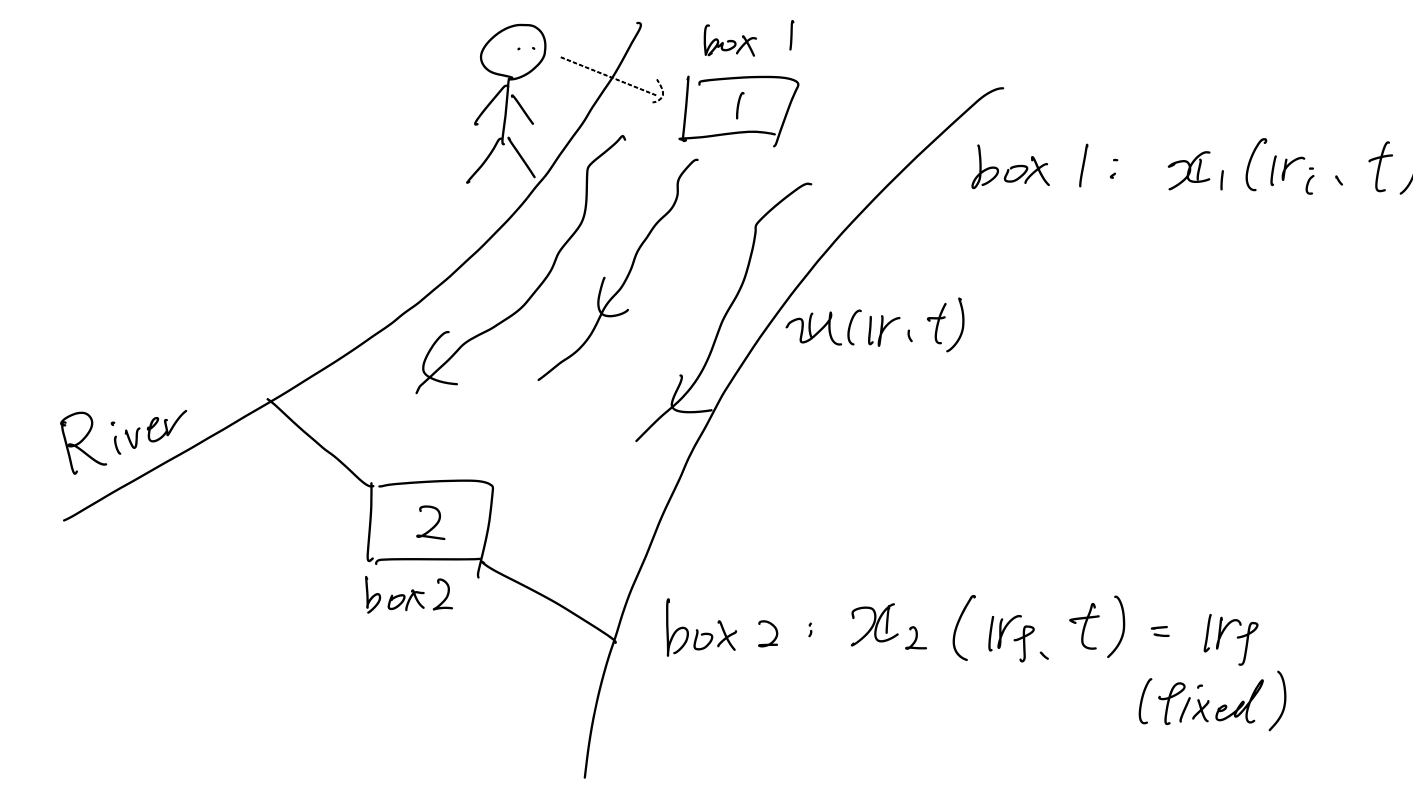
\includegraphics[width=0.45\textwidth]{images/am/river.png}
  \caption{Boxes on a river}
  \label{fig:lagrange_derivative}
\end{wrapfigure}
Since the water surface is not static, box 1 will be carried by the water flow.
Let us denote the position of the box 1 at time $t$ as $\vec{\xi} (\vec{r}_i, t; t_i)$, where the box 1 is placed at the point $\vec{r}_i$ at time $t_i$.

Let us denote the height of the water surface at a point $\vec{r}$ at time $t$ by $X(\vec{r}, t)$.
Then, we can write the height of the water surface at the positions of box 1 and 2 at time $t$ as
\begin{align}
  X(\vec{\xi}, t) & = X_1(t) \\
  X(\vec{r}_f, t) & = X_2(t)
\end{align}
Finally, assume that the box 1 will reach $\vec{r}_f$ at time $t_f$.

Now, at initial time $t_i$, the change in height of the water surface is given by:
\begin{align}
  X(\vec{r}_f, t_i) - X(\vec{r}_i, t_i) & = \nabla X(\vec{r}_i, t_i) \cdot (\vec{r}_f - \vec{r}_i) \\
                                        & = \nabla X(\vec{r}_i, t_i) \cdot \Delta \vec{r}
\end{align}
assuming that $\Delta \vec{r} := \vec{r}_f - \vec{r}_i$ is small enough.
On the other hand, for box 2, the change in height of the water surface in a time interval $\Delta t = t_f - t_i$ is given by:
\begin{align}
  X(\vec{r}_f, t_f) - X(\vec{r}_f, t_i) & = \pdv{X(\vec{r}_f, t_i)}{t} \Delta t
\end{align}
Thus, the total change of $X$ measured by box 1, during $\Delta t$, moving at the velocity $\vec{u}$ is given by
\begin{align}
  X(\vec{r}_f, t_f) - X(\vec{r}_i, t_i)
   & = X(\vec{r}_f, t_f) \underbrace{
    - X(\vec{r}_f, t_i)
    + X(\vec{r}_f, t_i)
  }_{=0} - X(\vec{r}_i, t_i)                                               \\
   & = \pdv{X}{t} \Delta t + \nabla X(\vec{r}_i, t_i) \cdot \Delta \vec{r}
\end{align}
Now, since $\vec{r}_i = \vec{\xi}(\vec{r}_i, t_i)$ and $\vec{r}_f = \vec{\xi}(\vec{r}_i, t_f)$, we can rewrite the equation above:
\begin{align}
  X(\vec{\xi}(\vec{r}_i, t_f), t_f) - X(\vec{\xi}, t_i) & = \pdv{X}{t} \Delta t + \nabla X(\vec{\xi}, t_i) \cdot \Delta \vec{\xi}
\end{align}
where $\Delta \vec{\xi} = \vec{\xi}(\vec{r}_i, t_f) - \vec{\xi}(\vec{r}_i, t_i)$.

Using $\Delta t = t_f - t_i$, we can rewrite the equation above as:
\begin{align}
  \frac{X(\vec{\xi} + \Delta \vec{\xi}, t_i + \Delta t) - X(\vec{\xi}, t_i)}{\Delta t}
   & = \pdv{X}{t} + \nabla X(\vec{\xi}, t_i) \cdot \frac{\Delta \vec{\xi}}{\Delta t} \\
\end{align}
Since the box 1 is a part of the fluid, the time derivative of $\vec{\xi}$ is the velocity of the fluid at the position $\vec{\xi}$:
\begin{align}
  \pdv{\vec{\xi}(\vec{r}_i, t)}{t} & = \vec{u}(\vec{\xi}, t)
\end{align}
\nt{
  In this derivative, we fix the starting position $\vec{r}_i$, we only care about the time evolution from the position $\vec{r}_i$.
  This is different from the total derivative, which takes into account a change in the starting position $\vec{r}_i$.
}
thus, by taking $\Delta t \to 0 (\implies \Delta x \to 0)$, we can rewrite the equation above as:
\begin{align}
  \mdv{X(\vec{\xi}, t_i)}{t} & := \pdv{X(\vec{\xi}, t_i)}{t} + \vec{u}(\vec{\xi}, t_i) \cdot  \nabla X(\vec{\xi}, t_i)
\end{align}
where $\mdv{}{t}$ indicates that we are tracking the box 1 and its measurement of $X$.
This is called the \emph{Lagrange derivative}:
\dfn{Lagrange Derivative}{
  The Lagrange description in Eulerian perspective is given as the \emph{Lagrange derivative}:
  \begin{align}
    \mdv{X}{t} := \pdv{X}{t} + \vec{u} \cdot \nabla X
  \end{align}
  which tracks the change of a physical quantity $X$ with the flow.
}

Now, define a new quantity called the "position function" $\vec{x}(\vec{r}, t)$:
\begin{align}
  \vec{x}(\vec{r}, t) & := \vec{r}
\end{align}
If we measure this position function at the box 1 at $t = t_i$,
\begin{align}
  \vec{x}(\vec{r}_i, t_i) & = \vec{r}_i
\end{align}
and notice that tracking the position of box 1 is equivalent to observing the time-evolved position $\xi(\vec{r}_i, t_i)$:
\begin{align}
  \pdv{\vec{\xi}}{t} & = \mdv{\vec{x}}{t} = \vec{u}(\vec{x}, t)
\end{align}

\subsection{Derivation from Action Integral}
In Newtonian mechanics, for a particle of mass $m$, the action integral $S$ is given by:
\begin{align}
  S & = \int \odif{t} \, L = \int \odif{t} \, m \lagr, \quad \lagr := \frac{L}{m} = \bab{\frac{1}{2} \dot{\vec{x}}^{\, 2} - \tilde{V}(\vec{x})}
\end{align}
where $\lagr$ is the Lagrangian density, and
\begin{align}
  \tilde{V}(\vec{x}) & = \frac{V(\vec{x})}{m}
\end{align}
by assuming a similar form of the Lagrangian density for a fluid, we can write the action integral for a fluid as:
\begin{align}
  S & = \int \odif{t} \, L = \int \odif{t} \, \int_V \rho(\vec{x}, t) \odif{V}(\vec{x}, t) \, \lagr\pab{\vec{x}, \mdv{\vec{x}}{t}}
\end{align}
where the Lagrangian density is
\begin{align}
  \lagr \pab{\vec{x}(\vec{r}, t), \mdv{\vec{x}(\vec{r}, t)}{t}} & = \frac{1}{2} \pab{\mdv{\vec{x}(\vec{r}, t)}{t}}^2 - \tilde{V}(\vec{x}(\vec{r}, t)) + \frac{1}{\rho(\vec{r}, t)} \nabla \cdot \sigma(\vec{r}, t) \vec{x}(\vec{r}, t)
\end{align}
Then the Euler-Lagrange equation for this Lagrangian density is given by:
\begin{align}
  \pdv{\lagr}{\vec{x}} - \mdv{}{t} \pab{\pdv{\lagr}{\pab{\mdv{\vec{x}}{t}}}} & = 0
\end{align}
calculating the partial derivative gives:
\begin{align}
  \pdv{\lagr}{\vec{x}}                & = \frac{1}{\rho} \nabla \cdot \sigma - \nabla \tilde{V}(\vec{x}) = \frac{1}{\rho} \nabla \cdot \sigma + \vec{\tilde{F}} \\
  \pdv{\lagr}{\pab{\mdv{\vec{x}}{t}}} & = \mdv{\vec{x}}{t} = \vec{u}(\vec{x}, t)
\end{align}
hence the Euler-Lagrange equation becomes:
\begin{align}
  \mdv{\vec{u}}{t} & = \frac{1}{\rho} \nabla \cdot \sigma + \vec{\tilde{F}}
\end{align}
by integrating over the volume $V$, we get
\begin{align}
  \int_V \rho \odif{V} \, \mdv{\vec{u}}{t}                & = \int_V \odif{V} \, \nabla \cdot \sigma + \int_V \rho \odif{V} \, \vec{\tilde{F}}  \\
  \implies \quad \int_V \rho \odif{V} \, \mdv{\vec{u}}{t} & = \int_V \odif{s} \, \vec{n} \cdot \sigma + \int_V \rho \odif{V} \, \vec{\tilde{F}}
\end{align}


\subsection{Hamilton Formalism}
Similarly to the point mass case, we should define the momentum density $\vec{\pi}(\vec{r}, t)$ as the derivative of the Lagrangian density with respect to the velocity:
\begin{align}
  \vec{\pi} (\vec{r}, t) & = \pdv{\lagr}{\pab{\mdv{\vec{x}}{t}}}
\end{align}
then the Hamiltonian density should be defined by the Legendre transformation:
\begin{align}
  \hami(\vec{\pi}, \vec{x}) & = \vec{\pi} \cdot \mdv{\vec{x}}{t} - \lagr \pab{\vec{x}, \mdv{\vec{x}}{t}}                               \\
                            & = \frac{1}{2} \pab{\mdv{\vec{x}}{t}}^2 + \tilde{V}(\vec{x}) - \frac{1}{\rho} \nabla \cdot \sigma \vec{x}
\end{align}


\cite{suzuki-leastActionFluid}




\section{Physical Constants}
All values are taken from \href{https://physics.nist.gov/cuu/Constants/index.html}{\emph{The NIST Reference on Constants, Units, and Uncertainty}} \cite{NIST-const}.
\begin{table}[htbp]
  \centering
  \caption{Physical Constants}
  \label{tab:physical_constants}
  \begin{tabular}{ccS[table-format=+1.9e+2]c}
    \toprule
    \textbf{Symbol}           & \textbf{Constant}        & {\textbf{Value}}  & \textbf{Units}                                  \\
    \midrule
    $c$                       & Speed of light in vacuum & 2.99792458e8      & \si{\meter\per\second}                          \\
    $e$                       & Elementary charge        & - 1.602176634e-19 & \si{\coulomb}                                   \\
    $G$                       & Gravitational constant   & 6.67430e-11       & \si{\newton\meter\squared\per\kilogram\squared} \\
    $h$                       & Planck constant          & 6.626 070 15e-34  & \si{\joule\second}                              \\
    $\hbar := \frac{h}{2\pi}$ & Reduced Planck constant  & 1.054 571 817e-34 & \si{\joule\second}                              \\
    \bottomrule
  \end{tabular}
\end{table}

% Textbooks
\newpage
\section{Textbooks}
\subsection{General Textbooks}
\begin{itemize}
  \item \emph{University Physics with Modern Physics} by Hugh Young and Roger Freedman \cite{young-freedman}
  \item \emph{Feynman Lectures on Physics} by Richard P. Feynman \cite{feynman-lectures-online}
\end{itemize}

\subsection{Analytical Mechanics}
\begin{itemize}
  \item \emph{Classical Mechanics} by Goldstein, Poole, and Safko \cite{goldstein-classical}
  \item \emph{Mechanics} by Landau and Lifshitz \cite{landau-mechanics}
\end{itemize}

\subsection{Quantum Mechanics}
\begin{itemize}
  \item \emph{Quantum Mechanics} by Leonard Schiff \cite{schiff}
  \item \emph{Introduction to Quantum Mechanics} by David Griffiths \cite{griffiths-qm}
  \item \emph{Modern Quantum Mechanics} by J. J. Sakurai and Jim Napolitano \cite{jjsakurai-qm}
\end{itemize}


\subsection{Particle Physics}
\begin{itemize}
  \item \emph{Introduction to Elementary Particles} by David Griffiths \cite{griffith-introToEP}
  \item \emph{An Introduction to Quantum Field Theory} by Michael Peskin and Daniel Schroeder \cite{peskin-introToQFT}
\end{itemize}

\backmatter
% Bibliography 
\renewcommand{\emph}[1]{\textit{#1}}
\printbibliography

\end{document}
